%% This is the preambule for the dissertation and the main document.
%% Global options and global packages will be stated here.
%% Then all preliminary pages and each chapter will be collated here.

%% Global options and packages:
\documentclass[12pt,letterpaper]{report} % This is not the correct page size!!
\usepackage[utf8]{inputenc}
\usepackage[english]{babel}
%% To include the math symbols ad formulas:
\usepackage{amsmath}
\usepackage{amsfonts}
\usepackage{amssymb}
%% To deal with the figures:
\usepackage{graphicx}
\graphicspath{{./fig/}} % Set the path for the figures.
%% To make the table with automatic line breaks:
\usepackage{tabularx}
%% The bibliography package:
\usepackage{natbib}
%% To change the line spacing:
\usepackage{setspace}
%% The hidelinks option will hide those green squares around the citations.
\usepackage[hidelinks]{hyperref}

% Allows extra dots between subheadings in TOC
\usepackage{tocloft}
\usepackage{titlesec}
% \title{Title}

% Changes the name of the table of contents:
\addto\captionsenglish{% Replace "english" with the language you use
  \renewcommand{\contentsname}%
    {Table of Contents}%
}

% Changes the font of the table of contents and the list of tables and figures.
\renewcommand{\cfttoctitlefont}{\normalfont\large\bfseries}
\renewcommand{\cftloftitlefont}{\normalfont\large\bfseries}
\renewcommand{\cftlottitlefont}{\normalfont\large\bfseries}

% Changes the white space before the table of contents and the list of tables and figures.
\setlength{\cftbeforetoctitleskip}{-13pt}
\setlength{\cftbeforeloftitleskip}{-13pt}
\setlength{\cftbeforelottitleskip}{-13pt}

% Changes the white space after the table of contents and the list of tables and figures.
\setlength{\cftaftertoctitleskip}{5pt}
\setlength{\cftafterloftitleskip}{5pt}
\setlength{\cftafterlottitleskip}{5pt}

% The 'titleformat' and 'titlespacing' commands take care of the formating for all sections.
% Here 'titleformat' changes the font and style of the section whereas 'titlespacing' will modify the space before and after the section. Very useful!
%\titleformat{\chapter}[block]{\large\bfseries\uppercase}{Chapter \thechapter :}{4pt}{}{}
\titleformat{\chapter}[block]{\large\bfseries}{CHAPTER \thechapter :}{4pt}{}{}
\titlespacing{\chapter}{0pt}{-20pt}{1cm}
\titleformat*{\section}{\large\bfseries}%
\titleformat*{\subsection}{\large\itshape}%
\titleformat*{\subsubsection}{\itshape}%

% Adds required dots between sections and page numbers in TOC
\renewcommand{\cftsecleader}{\cftdotfill{\cftsecdotsep}}
\renewcommand\cftsecdotsep{\cftdot}
\renewcommand\cftsubsecdotsep{\cftdot}
\renewcommand{\cftpartleader}{\cftdotfill{\cftdot}} % for parts
\renewcommand{\cftchapleader}{\cftdotfill{\cftdot}} % for chapters

%Clears plain-page pg# settings, relocates pg#'s @ top-right-corner.
\makeatletter
\renewcommand{\ps@plain}{
\renewcommand\@oddhead{\hfill\normalfont\textrm{\thepage}}
\renewcommand\@evenhead{}
\renewcommand\@oddfoot{}
\renewcommand\@evenfoot{}}
\makeatother

%Changes leading pg#'s to roman sytle
\renewcommand{\thepage}{\roman{page}}

%Changes default indenting in list of figures to 0 
\makeatletter
\renewcommand*\l@figure{\@dottedtocline{1}{0em}{2.3em}}% Default: 1.5em/2.3em
\let\l@table\l@figure
\makeatother

%Margins
\addtolength{\voffset}{-.5in}
\addtolength{\hoffset}{-.25in}
\setlength{\marginparwidth}{1in}
\setlength{\oddsidemargin}{.375in}
\setlength{\marginparsep}{0in}
\setlength{\topmargin}{12pt}
\setlength{\headheight}{12pt}
\setlength{\headsep}{20pt}
\setlength{\textheight}{9in}
\setlength{\textwidth}{6.5in}
\setlength{\footskip}{0in}

%Sets all text to double space, per \usepackage{setspace} 
%\doublespacing
\onehalfspacing

% Names list of figures and table of contents explicitly and sets spacing above and below titles
\renewcommand{\listfigurename}{\vspace{-2.2cm} \large List of Figures \vspace{-1cm}}
\renewcommand{\listtablename}{\vspace{-2.2cm} \large List of Tables \vspace{-1cm}}
\renewcommand{\contentsname}{\vspace{-2.2cm} \large Table of Contents \vspace{-1cm}}

%% List of words that cannot be hyphenated or which hyphenation need to be defined.
\hyphenation{Anolis}

\begin{document}

%% First the preliminary pages for the dissertation document.
%Sets non-header pages to same format (location) as header pages, e.g upper-right.
\pagestyle{myheadings}

%Clears pg# from displaying on titlepage
\thispagestyle{empty}

%Titlepage
\begin{center}
Challenges and advances for phylogenetic comparative models of trait evolution\\
\vspace{48pt}
A Dissertation\\
Presented in Partial Fulfilment of the Requirements for the\\
Degree of Doctorate of Philosophy\\
with a\\
Major in Bioinformatics and Computational Biology\\
in the\\
College of Graduate Studies\\
University of Idaho\\
by\\
Daniel Caetano da Silva\\
\vspace{60pt}
Major Professor: Luke Harmon, Ph.D.\\
Committee Members: David Tank, Ph.D.; Jack Sullivan, Ph.D.; Paul Hohenlohe, Ph.D.\\
Department Administrator: Eva Top, Ph.D.\\
\vspace{80pt}
August 2017\\
\end{center}
\pagebreak

%Authorization to Submit Thesis
\addcontentsline{toc}{chapter}{Authorization to Submit Thesis} % Line to add the entry to the table of contents.
\section*{\large{Authorization to Submit Thesis}}
\begin{flushleft}
This dissertation of Daniel Caetano da Silva, submitted for the degree of Doctorate of Philosophy with a major in Bioinformatics and Computational Biology and titled ``Challenges and advances for phylogenetic comparative models of trait evolution," has been reviewed in final form. Permission, as indicated by the signatures and dates given below, is now granted to submit final copies to the College of Graduate Studies for approval.
\end{flushleft}
\begin{singlespace}
\ \ \ \ \ Major Professor:\indent\underline{\makebox[2.8in][l]{\ }}Date\underline{\makebox[1.2in][l]{\ }}\\
\ \ \indent\indent\indent\indent\indent\indent\indent Luke Harmon, Ph.D.\\
\ \\
\ \ \ \indent Committee\\
\ \ \ \indent Members:\indent\indent\ \ \ \ \ \underline{\makebox[2.8in][l]{\ }}Date\underline{\makebox[1.2in][l]{\ }}\\
\ \ \indent\indent\indent\indent\indent\indent\indent David Tank, Ph.D.\\
\ \\
\ \ \indent\indent\indent\indent\indent\indent\ \ \ \ \underline{\makebox[2.8in][l]{\ }}Date\underline{\makebox[1.2in][l]{\ }}\\
\ \ \indent\indent\indent\indent\indent\indent\indent Jack Sullivan, Ph.D.\\
\ \\
\ \ \indent\indent\indent\indent\indent\indent\ \ \ \ \underline{\makebox[2.8in][l]{\ }}Date\underline{\makebox[1.2in][l]{\ }}\\
\ \ \indent\indent\indent\indent\indent\indent\indent Paul Hohenlohe, Ph.D.\\
\ \\
\ \ \indent Department\\
\ \ \indent Administrator:\ \ \ \ \ \ \ \underline{\makebox[2.8in][l]{\ }}Date\underline{\makebox[1.2in][l]{\ }}\\
\ \ \indent\indent\indent\indent\indent\indent\indent Eva Top, Ph.D.\\

\end{singlespace}
\pagebreak

%Abstract
\addcontentsline{toc}{chapter}{Abstract}
\section*{\large{Abstract}}

A phylogenetic tree is a hypothesis of evolutionary relationships among lineages. The branching pattern of such tree tells us the history of groups of species derived from their common ancestors. The length of each branch of this tree represent time, a critical information to study evolutionary processes. Such a tree is the starting point for phylogenetic comparative studies, which aim is to use phylogenies to test hypotheses about macroevolution. On a broad scale, comparative studies can be divided between the study of pattern and processes of lineage diversification and trait evolution. For example, whether the first is concerned with why beetles are one of the most diverse groups among all animals, the latter is intrigued by the beetles' diversity of shapes, sizes, and colors. This dissertation will focus on macroevolutionary patterns and processes underlying phenotypic evolution, especially on identifying challenges and providing advances regarding such analyses.

Here I use and develop statistical models to ask questions such as the association between morphological differentiation and lineage diversification and patterns of evolutionary correlation among several traits. The present dissertation is divided into four chapters. The first tests whether the coloration pattern associated with Neotropical false-coral snakes of the family Dipsadidae has a positive effect on the rates of diversification of the group. For this I collected coloration information for more than 600 species of snakes from a diverse array of sources, including taxonomic descriptions, photos, and direct observations of live and preserved specimens. Then I used the phylogenetic tree of the group to fit a binary state speciation and extiction model (BiSSE) that simultaneously estimates rates of color evolution and associate each color type with diversification rates. After thoughtfully exploring the results due to the known biases associated with this method and applying several additional analysis I concluded that the signal for a dependence between coloration type and diversification of the group is weak. This chapter exemplifies the need for careful exploration of the different factors that might influence any macroevolutionary analysis using phylogenetic trees.

In the second chapter I focused on evolutionary modularity and developed a novel Bayesian approach to study patters of evolutionary correlation among several continuous traits using Markov-chain Monte Carlo. Evolutionary modularity is defined as the pattern in which evolutionary changes of one trait is correlated with evolutionary changes of another trait. The model used in this chapter is based on the evolutionary rate matrix which is a variance-covariance matrix with dimensions equal to the number of traits. The diagonal elements of such matrix have the evolutionary rate for each of the traits whereas the off-diagonals show the pairwise evolutionary covariances. Then, one can use the pairwise covariances in order to study the pattern of evolutionary modularity among continuous traits. In this chapter I also contrast results based on a point estimate of the evolutionary rate matrix using maximum likelihood and the posterior distribution of Bayesian analyses. I show that the lack of uncertainty around parameter estimates under maximum likelihood can bias results since likelihood ratio tests do not take into account the variance around the parameter estimates for the model.

The third chapter is composed by the implementation of the new method described on the second chapter in the widely used programming language and statistical environment R. The package is named \texttt{ratematrix} and it presents a novel approach to deal with the proposal of new variance-covariance matrices for Markov-chain Monte Carlo analyses. The approach separates the variance-covariance matrix into a correlation matrix and a vector of variances. This separation make it possible to explore the parameter space in a more efficient manner while also preventing the proposal of matrices that do not follow the mathematical rules which define a variance-covariance matrix. In this same chapter, I also developed and implemented an extension of Felsenstein's pruning algorithm applied when multiple independent multivariate Brownian-motion rate regimes are fitted to the same phylogenetic tree. This advance of the classic pruning algorithm makes it possible to compute the likelihood of models including a large number of species and traits, since previous implementations suffered from the strong limitations associated with inverting very large matrices.

The fourth chapter introduces the use of mathematical functions to describe the heterogeneity in the rate of evolution of one continuous trait across the branches of a phylogeny as predicted by another trait. Here I developed a new phylogenetic comparative method that utilizes predictive mathematical functions to describe a gradient of rates of evolution for a continuous response trait based on the trait values of a predictor continuous trait mapped to the phylogenetic tree. This approach make it possible to test whether the tempo of macroevolution of a trait is influenced by the gradient of another trait. I also conducted a series of simulations to show that the method can successfully recover the parameter values that generated the data and shows good performance.

In summary, in this dissertation I visit different topics associated with phylogenetic comparative models of trait evolution. Each chapter focus on a current challenge in phylogenetic comparative studies; the association of trait with rates of diversification on chapter one, simultaneous study of several traits on chapters two and three and the correlation between rates of evolution and a potential predictor trait on chapter four. Throughout this dissertation I introduce many advances to the field, especially with respect to the implementation of new models, algorithms, software and the critical evaluation of current practices.

\pagebreak

%Acknowledgements
\addcontentsline{toc}{chapter}{Acknowledgements}
\section*{\large{Acknowledgements}}

\ \ \ \ \ It is not easy to forget the process of moving from Sao Paulo (Brazil) to Moscow (USA). Such a decision represented for me the best move I could ever make in my career. For the American reader I want to ask you to look around and imagine that your profession of choice is conducted in another language. Now also try to think that the next big conference in your field will be overseas, the next also, and the other too. You now also have to worry if a reviewer will ask whether a native speaker reviewed your writing before sending your manuscript to review. That is reality on the majority of countries around the world that do science and everyday concerns for both students and faculty. So, yes, coming to US to pursue my doctorate degree was a big thing.

Fortunately, all the anxiety that I felt after realizing the size of Moscow, ID, went away when I started working with the fantastic community of evolutionary biologists at the University of Idaho. The frequent interactions with students and faculty makes this place warm to the heart, more than a necessity given the extreme low temperatures during the dark afternoons of winter. The constant open conversation and clear focus on scientific arguments rather than academic hierarchies makes any student feel as part of something bigger. This environment makes us want to grow and to develop as far as we can. The whole department should be proud of the energy that it transmits.

This is also a place of routine, but in a good way. The schedule of the week is quite clear: work, PEES, IBEST Lunch, meet the speaker, and, of course, the Friday: PURGE, check email, Biology seminar, and... is already 5PM, so beers. I am guilty of complaints about so many things to do sometimes. However, I am sure that I am going to miss all this so much! Among all the things, PURGE will have the longest mark on me, both as a person and as a professional. The opportunity of discussing published articles with fellow students and professors weekly is just fantastic! I learned so much with everyone. Learned that it is good to know and even better to know you don't know. Learned to listen and make yourself listened. And, of course, the occasional practice of talking about a manuscript you failed to read will, I am sure, be handy some day.

The colleagues, collaborators and friends that made me company on this five years journey also deserve many thanks. Professors Luke Harmon, Dave Tank and Jack Sullivan were always there to discuss any topic and for this I am hugely grateful. The Harmon lab, my home, is a group of big ideas and bold projects. I learned a lot from all lab-mates. Thanks to Matt Pennell for helping me with all the first steps as a graduate student and to inspire (also provoke) me to pursue big accomplishments. Thanks Denim Jochimsen for helping me with all the snake-things. Many thanks to Rafael Maia and Eliot Miller, was super cool to have you in the lab and bring much more diversity of topics to the table. Special thanks to Rosana Zenil-Ferguson for raising the level of the statistical work of everyone in the lab and for the patience to explain all the things. Another super special thanks to Josef Uyeda. I am happy to say that Josef is a model of the scientist I hope one day to be and I am super proud of having shared a lot of ideas and beers with you. Finally, my big thanks to Luke Harmon! I am still impressed with how luck I was to have the opportunity to join your team. Being your student was an amazing experience and a very important turning point in my academic career. I will aim high and do all the things Luke, I promise!

Many thanks to the Tank lab, my second home, and all the plant people that effectively help the Harmon lab to keep things real. Since Dave Tank moved to the Biology Department it has been great to have him around. You helped me a lot Dave, thanks! Thanks to Hannah Marx and Simon Uribe-Convers, both PhDs for some time already. Many thanks also to Diego Morales-Briones and Sarah Jacobs for making me company in the office, discussing all the science and also having all the fun. Many thanks also to Megan Ruffley, Ian Gilman and Sebastian Mortimer, you are all great and wish all the good things for your next steps!

And, of course, many thanks to the Moscow crew! Too many names to list but, hey, you know all who you are. See you at BBBBBBBBBB!!

\pagebreak

%Dedication
\addcontentsline{toc}{chapter}{Dedication}
\vspace*{\fill} % This centers the text vertically
\begin{center} % This centers the text horizontally

\begin{large}
\textbf{Dedication} \\
\end{large}
\indent To my parents for all the effort in providing me more that they ever had. \\
\indent All that I got and will get is because of their support, patience and love. \\
\indent Para meus pais por todo o esforço para me dar muito mais do que eles tiveram na vida. \\
\indent Tudo o que consegui até hoje foi por causa do seu apoio, paciência e amor.

\end{center}
\vspace*{\fill}
\pagebreak

%Table of Contents
\addcontentsline{toc}{chapter}{Table of Contents}
\tableofcontents
\pagebreak

%List of Tables
\addcontentsline{toc}{chapter}{List of Tables}
\listoftables
\pagebreak

%List of Figures
\addcontentsline{toc}{chapter}{List of Figures}
\listoffigures
\pagebreak

%Sets page count at one
\setcounter{page}{1}
%Sets pg# type to display arabic numerals
\renewcommand{\thepage}{\arabic{page}}

%% Now these are the chapters for the dissertation
%% Need to make some modifications. Figures that were Suplementary now need to be main text. 
%% This is the chapter 1. This chapter will need to be translated from a word document to the Latex.
%% It will give a little more of work. Not that much, I think.

\chapter{HAVE CORAL SNAKE MIMICS DIVERSIFIED MORE THAN NON-MIMICS?}

\section{Abstract}

Dipsadidae is one of the most diversified family of snakes, composed of species showing an impressive variety of color patterns. Some species are cryptic whereas others have contrasting patterns comprised by bright colors alternated with darker shades, including particular combinations of vivid colors characteristic of coral snakes (Elapidae). Species with such patterns are thought to be mimics of coral snakes based on their color pattern similarity, predator avoidance of such patterns in field experiments, and the geographical concordance between models and mimics. Here we test whether color patterns associated with coral snake mimicry and contrasting color patterns in general influenced the diversification dynamics of the group. We compile a large database of color patterns with color descriptions for about 80\% of the known diversity of the group (594 species). We used trait-dependent diversification models along with extensive simulations to deal with the recently described statistical bias associated with such methods. We also tested whether color patterns are associated with trait-independent estimates of diversification. Despite the apparent survival advantage associated with coral snake mimicry, we show that there is no detectable influence of color types in the dynamics of diversification in Dipsadidae and discuss insights into the potential functions of color patterns.

\section{Introduction}

Colors play an important role in avoiding predation. Patterns similar to the background environment make prey difficult for the predators to detect and recognize \citep{merilaita_2005, stevens_2009}. On the other hand, bright and contrasting colors displayed by unpalatable, toxic or venomous animals (i.e., aposematic patterns) serve as warning signals that are often avoided by visually oriented predators \citep{wallace_1867, mappes_2005, speed_2005}. However, such conspicuous colors can also be displayed by mimics, which gain protection by deceiving predators that avoid their false warning signals. Strong evidence from field experiments shows that mimicry of warning signals decreases predation pressure when compared to cryptic color patterns \citep{jeffords_batesian_1979, brodie_differential_1993, brodie_experimental_1995, pfennig_2001, pinheiro_2011, pfennig_2015}. Such reduction in predation pressure may also have positive impacts on habitat use by aposematic lineages and their mimics. Cryptic animals are to some degree restricted to backgrounds which their color patterns match and may only be active at certain times because movement is often antithetic to good crypsis \citep{speed_2010, stevens_2012}. In contrast, such restrictions may be weaker in aposematic or mimic lineages, which could promote more opportunities to exploit habitat resources \citep{speed_2010}.

In contrast with aposematism, the survival advantage of Batesian mimicry is dependent on the relationship between the model and the mimetic organism because predators need to associate the unpalatability or hazard of the model with the warning signals of the deceiver. Once this association is broken, a mimicry breakdown occurs and the mimic phenotype might become maladaptive since warning signals can make individuals more conspicuous to predators \citep{mallet_evolution_1999, pfennig_2001, pfennig_2015}. Mimicry breakdown can be caused by allopatry between mimic and model populations as a result of population expansion of the mimic or local extinction of the model \citep{pfennig_2010}. Allopatric mimics are conspicuous to naïve predators that might not avoid their deceptive warning signals and this may result in higher predation rates and eventual extinction of the mimic population \citep{pfennig_2015}. On the other hand, population expansion or migration of mimics can create opportunities for local adaptation to novel aposematic models. This process could result in selection against intermediate hybrids followed by decreased gene flow among populations and eventually promote reproductive isolation \citep{mallet_evolution_1999, pfennig_2015}. Over longer time scales such processes might have a positive effect on rates of diversification of mimetic lineages. Previous studies show that aposematic lineages are more species-rich than cryptic ones \citep{santos_2003, przeczek_2008}, suggesting that the evolution of the aposematic condition may even represent a key innovation \citep{speed_2010}. This key innovation hypothesis could be extended to mimicry; however, the potential effects of mimicry evolution on lineage diversification have yet to be investigated.

Among snakes, groups of relatively harmless or mildly venomous species showing color patterns similar to those of venomous coral snakes (Elapidae) have instigated a long debate on whether such patterns are mimetic \citep[see a comprehensive review in][]{pough_1988}. Reports often rely on the similarity of color patterns between mimics and models to argue in favor of mimicry relationships \citep{dunn_coral_1954, hecht_coral_1956, greene_coral_1981, savage_1992}. Additional evidence come from parallel geographic variation of coral snakes and their putative mimics \citep[e. g.,][]{hecht_coral_1956, zweifel_1960, greene_coral_1981, marques_1991, rabosky_coral_2016} and from field studies using replicas of coral snakes and other similar color patterns \citep{smith_1975, brodie_differential_1993, brodie_experimental_1995, hinman_predation_1997, pfennig_2001, buasso_predation_2006}.

Some authors pointed to the possibility that contrasting colors, including the stereotypical banded pattern observed in almost all coral snakes, could serve a disruptive function \citep{gadow_1908, thayer_1909, dunn_coral_1954, brattstrom_coral_1955}. Those reports suggested that the alternate pattern of bands could blend to the background environment and break the outline of the snake body, making recognition by visually oriented predators difficult. Recently, Titcomb and colleagues \citeyear{titcomb_2014} showed that the contrasting ringed pattern of coral snake mimics can create an illusory effect when the individuals are moving fast. The effect, called flicker-fusion, can give advantage to snakes against avian predators independent of mimicry. Despite its protective effect, the plausible disruptive function of the contrasting bands do not invalidate the existence of a mimicry complex between elapids and snakes from other families, since the same color pattern can perform both functions \citep{titcomb_2014}.

The family Dipsadidae (\citealp{zaher_2009}, \textit{sensu} \citealp{grazziotin_molecular_2012}) is a diverse group of snakes, with ca. 700 species occurring from Central to South America \citep{grazziotin_molecular_2012, uetz_2014}, and is characterized by an impressive variety of color patterns \citep[see][for some examples]{martins_1998}. Some dipsadids have color patterns similar to those of coral snakes, and have long been suggested as cases of mimicry of New World coral snakes \citep[family Elapidae;][]{wallace_1867, greene_coral_1981, sazima_1991, savage_1992, martins_1993, pough_1988, almeida_morphological_2014}. The contrasting coloration found in dipsadid snakes always includes bright colors but is not restricted to ringed patterns. In general, species can vary from the coral snake pattern of black, red and yellow rings or bands to a less colorful homogeneous red body with a single black or cream band on the neck (nuchal collar). Besides contrasting color patterns, the family also shows a diverse array of cryptic color patterns, characterized by blotches and shades of brown, gray, or green. Included in the latter are species whose dorsum is cryptic and whose venter has a plain bright color and even a coral snake pattern. Mimetic and cryptic patterns can be found both within and among genera and make dipsadid snakes an ideal study system to investigate the possible effects of such distinct color types on macroevolutionary patterns.

Herein we test whether distinct color patterns have an influence on the diversification of the family Dipsadidae. We investigate whether color patterns similar to coral snakes (and contrasting color patterns in general) show diverging macroevolutionary patterns when compared to non-mimic and cryptic lineages, respectively. We show that there is no detectable influence of supposedly mimic or contrasting color patterns in the dynamics of diversification.

\section{Materials and Methods}

\subsection{Phylogenetic reconstruction}

We used sequence data for Dipsadidae and outgroup species previously analyzed by Grazziotin and colleagues (2012, see GenBank accession numbers in their Appendix S1). We aligned sequences using MAFFT \citep{katoh_mafft_2005} under the G-INS-i strategy and selected models of molecular evolution for each of the eight gene sequences using a decision theory framework in DT-ModSel \citep{minin_2003}. We concatenated the alignments and set four partitions; one partition for each nuclear gene (bdnf, c-mos, and rag2) and a single partition with the mitochondrial genes (12S, 16S, cytb, nd2, and nd4). We used phyutility \citep{smith_2008} to trim down all sites with 75\% or more missing data and inferred a Maximum Likelihood (ML) tree using GARLI 2.0 \citep{zwickl_2011}. We used the resulting ML phylogeny as the starting tree for three independent searches in BEAST 1.8 \citep{drummond_bayesian_2012} for 270 million generations with a thinning interval of 1500 generations each. Since there are sequences available for only few species of each genera we set an incomplete sampling birth-death tree prior \citep{stadler_2009} and an uncorrelated relaxed clock model to estimate relative branching times. We checked each run for convergence using Tracer 1.6 \citep{drummond_bayesian_2012} and excluded 50\% of the posterior chain as burnin. We then combined the posterior from the three BEAST searches and randomly sampled 100 trees, rescaled all trees to a total depth of 1, and retained only one randomly selected species of each genera while pruning the rest. When the original tree had paraphyletic genera we selected the most inclusive monophyletic clade representing each group and kept a single species to represent each of those genera. Then, we used the resulting pool of genus-level phylogenetic trees to perform all subsequent comparative analyses. The 100 sampled trees and the BEAST xml file comprising the data matrix, selected models of molecular evolution, starting tree and prior parameters is available in FigShare (http://dx.doi.org/10.6084/m9.figshare.831493). We also deposited the configuration and log files for GARLI 2.0. Figures \ref{fig:full_MCC1} and \ref{fig:full_MCC2} show the resulting maximum clade credibility (MCC) tree and respective posterior probability support values.

\subsection{Color patterns}

To understand the evolution of colors and its effect on diversification we compiled a large database of coloration patterns for dipsadid snakes. We searched several information sources such as comprehensive taxonomic reviews \citep[e.g.,][]{downs_1967}, published articles and books containing photographs of identified individuals \citep[e.g.,][]{savage_2002, campbell_lamar_2004}, trusted on-line photo repositories (e.g., CalPhotos - http://calphotos.berkeley.edu/ and Reptile Database – \citealp{uetz_2014}), photographs of live individuals, and museum specimens. We excluded invalid taxa or names presenting nomenclatural problems that are still appearing in the literature or online databases. We avoided subspecific ranks for coding the currently recognized taxa (with the exception of four subspecies of \textit{Alsophis antillensis}) because terminals in available phylogenies correspond to species only and less than 10\% of the members of the family Dipsadidae present valid subspecies to date.

While color diversity makes the family Dipsadidae interesting for studies focusing on the evolution of color patterns such as ours, this is also the most challenging characteristic of the system. Since it is not possible to consider all diversity of color patterns for comparative analyses, we used categories that are directly related to the hypotheses tested. For that, we describe below two distinct classifications of the color patterns, each one including a different important aspect of the biology of the group. We repeated all comparative analyses with each of these color pattern classifications in order to access how distinct interpretations of color diversity in the group affect our macroevolutinary conclusions.

First, we compared coral-mimics with non-mimics. We call coral-mimics species that resemble the color pattern of any New World coral snake species \citep[see][]{roze_1996, campbell_lamar_2004}. Species included in this category can show the coral-mimic pattern throughout the dorsum (e.g., \textit{Simophis rhinostoma}) or restricted to the anterior portion of the body (e.g., \textit{Pseudoboa coronata}). On the other hand, all species not defined as potential mimics of coral snakes, independent of whether their color pattern was better described as contrasting or cryptic, were included in the category of non-mimics. As a result, the non-mimic category comprise species with cryptic color patterns and others with bright coloration but not resembling any known lineage of New World coral snake. Second, we compared contrasting with cryptic species. We defined as contrasting species that show brightly colored patterns in general, independent of whether the color pattern was similar to those of coral snakes. The category coral-mimic is a subset of the contrasting category; every coral-mimic lineage is among the species defined as contrasting, but the reverse is not true. On the other hand, we defined as cryptic all color patterns lacking contrasting colors. Examples of such patterns are blotches with hues of brown, reddish brown, gray, and other combinations of dark colors. We also considered as cryptic species whose dorsum is homogeneously green, since individuals of those species are usually found among leaves of trees and bushes (e.g., \textit{Uromacer}).

There are three other important aspects of the color patterns in the group that could potentially affect our study; the presence of color polymorphism, ontogenetic changes in coloration and contrasting coloration restricted to the venter of the body. In the case of species with color polymorphism, some populations may show cryptic patterns occasionally associated to thermoregulation (\citealp{tanaka_2005}, but see \citealp{lorioux_2008}). Alternatively, contrasting colors in polymorphic populations can be due to increasing sexual dichromatism in the course of the reproductive season \citep{forsman_opposing_1995, lindell_1996}, related to non-selective processes, such as migration and dispersal \citep{king_color_1995} or genetic drift in local \citep{brakefield_genetic_1990} or island populations \citep{bittner_gene_2003}. Independent of the potential sources of the polymorphic color patterns we assigned species to the non-mimic and cryptic categories every time a cryptic morph was described among color types. Some Pseudoboini snakes \citep[\textit{sensu}][]{zaher_2009} show ontogenetic changes in color pattern in which juveniles are brightly colored but become cryptic when adults \citep{martins_1998}. We included those species into the contrasting category since juveniles correspond to the life stage most threatened by predation \citep{bonnet_dangers_1999} and thus their defensive tactics are fundamental for individuals to reach sexual maturity. Finally, some species show cryptic color patterns in the dorsum but have contrasting patterns restricted to the venter. The distinct patterns in the dorsum and venter are usually associated with a threatening display in which individuals twist the body and expose the bright colors when disturbed \citep{martins_1993, sawaya_2008, tozetti_2009}. Hence, we classified those cases into the contrasting category instead of following their dorsal coloration. We provide additional data with the list of species included in each of these cases. We also repeated comparative analyses with alternative color categories defined to accommodate such cases, but results showed no appreciable difference when compared to the coral-mimic vs. non-mimic or contrasting vs. cryptic categories.

\subsection{Comparative analyses}

In order to test whether color patterns influence the dynamics of diversification of Dipsadidae snakes we performed a series of complimentary phylogenetic comparative analyses using the pool of 100 trees sampled from the posterior distribution and the three distinct color pattern classifications defined above. We used the Binary State Speciation and Extinction model \citep[BiSSE –][]{maddison_2007, fitzjohn_estimating_2009, fitzjohn_2012} and the Hidden State Speciation and Extinction model \citep[HiSSE –][]{beaulieu_detecting_2016} followed by model adequacy simulations. Both BiSSE and HiSSE are joint models of trait and trees \citep{beaulieu_detecting_2016} because model parameters reflect diversification rates conditioned on the state of the traits and trait transitions throughout the tree. In addition, we estimated trait-independent diversification rates using BAMM \citep{rabosky_2014} and tested whether the distribution of color patterns across dipsadid genera is associated with the diversification dynamics of the group. We describe details for each analyses below.

Since a species-level tree is not available for the Dipsadidae family, we used the pool of genus-level trees as terminally unresolved trees \citep[\textit{sensu}][]{fitzjohn_estimating_2009} to estimate trait-dependent diversification using BiSSE. We used Markov chain Monte Carlo (MCMC) to estimate the posterior distribution of the parameters for the unconstrained BiSSE model (six free parameters) and the constrained model, in which $\lambda$ and $\mu$ are not related to color types (four free parameters). We used an exponential prior distribution with rate parameter equal to 0.3 for all BiSSE parameters and a starting point equal to the maximum likelihood estimate (MLE) for the model. We ran 10,000 generations of MCMC (chain length was based on preliminary analyses), discarded 50\% of generations as burnin and checked convergence using the `coda' package \citep{plummer_2006}. To test whether the full model explained the data better than the trait-independent model we performed model selection using the Bayesian Deviance Information Criteria \citep[DIC –][]{gelman_understanding_2013}. In order to account for the behavior of the BiSSE model when its assumptions are violated \citep{rabosky_2015, beaulieu_detecting_2016}, we did posterior predictive checks for model adequacy to test whether data simulated under the trait-dependent and trait-independent BiSSE models are similar to the observed data. For each model, we simulated traits using the `tree.bisse' function in the package `diversitree' \citep{fitzjohn_2012} with parameters drawn from the joint posterior distribution resulting from the BiSSE analysis and constraining simulations to have a tree depth equal to 1 (identical to the empirical trees). Then, we compared the number of species and the relative frequencies of each trait generated by the simulations with the empirical dataset. If models are adequate, simulated phylogenies should produce both diversity and frequency of states similar to the observed data.

Recently, \citet{beaulieu_detecting_2016} described the HiSSE model that introduces hidden states associated with each of the traits and helps to accommodate the rate heterogeneity observed on empirical phylogenetic trees \citep{rabosky_2015, beaulieu_detecting_2016}. The implementation of HiSSE integrates incomplete sampling using the proportion of known species associated with each trait across the whole tree, but does not include the option of terminally unresolved phylogenetic trees such as `diversitree' \citep{fitzjohn_2012}. We fitted the 20 trait-dependent (including BiSSE and HiSSE models) and 4 trait-independent models to each of the 100 genus-level phylogenetic trees and performed model choice among models fitted for each tree using the Akaike Information Criteria (AIC).

Finally, we used BAMM \citep{rabosky_2014} to estimate rates of diversification and shift locations in the tree independent of the trait data. Different from the BiSSE and HiSSE analyses, we used species-level phylogenies by randomly resolving the relationships within each genera using a constant rate Birth-Death model \citep{kuhn_simple_2011}. This approach assumes that diversification rates are homogeneous within each genera but should not bias the estimation of diversification rates for the backbone tree, since BAMM fits distinct rate regimes to different parts of the tree. Additionally, we set the BAMM model with constant rates through time within each regime \citep[similar to MEDUSA –][]{Alfaro_2009}, since this is a more adequate model given that diversification rates within genera were constrained to a homogeneous clock model. We set two independent MCMC chains for each of the 10 phylogenetic trees randomly sampled from the BEAST analysis. We ran each chain for 5 million generations, discarded 20\% of generations as burnin and checked convergence using the `coda' package \citep{plummer_2006}. Finally, we tested for a linear relationship between diversification rates and the proportion of each color pattern among species of each genera. Since there is large variation in species richness across the genera, we performed two analyses; the first including all genera with at least two species and the second excluding all genera with less than 10 species (total of 54 and 14 genera, respectively).

Recently, Moore and colleagues \citeyear{moore_2016} pointed out some important issues with BAMM's implementation; that the likelihood function does not incorporate diversification shifts on unobserved branches of the tree, that posterior estimates of the number of shifts is sensitive to the prior specification and that use of the compound Poisson process (CPP) prior make it difficult to differentiate many rate shifts of small effect from fewer rate shifts of large effect. Shortly after, Rabosky and colleagues \citeyear{rabosky_2017} responded to the critiques by showing that not incorporating shifts on unobserved branches has only minor impacts on inferences and argued that \citet{moore_2016} assessment of prior sensitivity on posterior estimates of the number of shifts was problematic. In this study, we use only relative diversification rates compared across genera (i.e., the slope of the regression) and our analyzes do not focus on the posterior distribution of the number of rate shifts across the tree. Thus, we believe that most concerns associated with BAMM should not have major impacts on our biological conclusions. Nevertheless, we repeated BAMM analyses with different prior distributions for the expected number of shifts ($\gamma$ = 0.1, 1, or 10) to test whether our results could be affected by the prior sensitivity.

We repeated all trait-dependent analyses with each of the three distinct color pattern categories. R scripts, BAMM files, phylogenetic trees and coloration data to reproduce all analyses are available in the github repository \url{https://github.com/Caetanods/Dipsadidae_color_evolution} .

\section{Results}

We compiled a large report of coloration descriptions for 594 species of dipsadid snakes covering over 80\% of the known diversity of the group. We were able to get detailed color descriptions for most species, but for some the information available was incomplete or limited (i.e., taxa known from a single specimen). Although those cases were not suitable for definition as coral-mimic or non-mimic lineages (i.e., state unknown or `NA'), we managed to classify those as either contrasting or cryptic for all but a few exceptions. Among all data sources, museum specimens are the most difficult to categorize since colors fade after preservation and only light and dark hues remain. Bright colors such as yellow, orange, pink, and red (derived from carotenoid pigments) fade completely over time turning into cream on preservative fluid. In contrast, dark pigmentation is preserved and sometimes turns into shades of black or dark brown. As a result, we assigned museum specimens with alternate bright and dark bands (or with a distinct nuchal collar) as contrasting and homogeneous light or dark patterns as cryptic. We provide the species list and their color patterns under the distinct categorization schemes in the online data repository ( \url{https://github.com/Caetanods/Dipsadidae_color_evolution} ).

We made analyses using BiSSE based on the two different categorizations of the same color description dataset (see Material and Methods). When we compared coral-mimic to non-mimic patterns, net diversification estimates associated with the coral-mimic trait ($\lambda_{1} - \mu_{1}$) were in average two times higher than non-mimics (Figure \ref{fig:diversity_phylo}). In contrast, when diversification rates are constrained to be independent of color types we recovered intermediate net diversification values relative to the trait-dependent model. These results are qualitatively similar to the analyses based on the contrasting and cryptic alternative categorization (Figure \ref{fig:par_BiSSE}). Both trait-independent and trait-dependent BiSSE models estimated strongly asymmetrical transition rates with changes from the coral-mimic to the non-mimic state ($q_{10}$) in average two to three times more frequent than the reverse ($q_{01}$). The median of the posterior distribution of transition rates are also qualitatively similar independent of color categorization (Figures \ref{fig:diversity_phylo} and \ref{fig:par_BiSSE}). These results were consistent across all sampled trees and the trait-dependent diversification model was the one preferred by the DIC model selection criteria independent of the phylogeny and the color categorization used in the analysis (Figures \ref{fig:dic_plot} and \ref{fig:model_select}).

We performed posterior predictive simulations to evaluate whether the BiSSE trait-dependent diversification model is adequate to explain the observed data. Since there is no appreciable difference in parameter estimates and DIC results across the categorizations of color types, we performed simulations based only in the contrasting vs. cryptic category. The posterior predictive simulations using both trait-dependent and trait-independent BiSSE models produced trees much smaller than the 594 species provided as the observed total diversity of the group (see left column of Figure \ref{fig:predic_BiSSE}). Since the stopping criteria for simulations were tree depth, the number of species in each simulated tree was free to vary. Trees simulated under the full model had on average 211 species and only 9\% of those showed more species than the observed data. Similarly, trees simulated using the trait-independent model had on average 186 species, of which only 5\% were larger than the observed data. With respect to trait frequency, both models simulated datasets biased towards higher frequencies of the cryptic color type. On average the full model had 67\% and the trait-independent model 84\% of the simulations showing frequencies of the cryptic color type higher than observed in the empirical data (see right column of Figure \ref{fig:predic_BiSSE}). Therefore, our results show that both BiSSE models have similar biases and the characteristics of the data not satisfactorily explained by the models are independent to whether rates of diversification are associated with color types or not.

The analyses comparing 16 HiSSE, 4 BiSSE, and 4 trait-independent models estimated using maximum likelihood resulted in only two variants of the BiSSE model selected as the best model across the sample of 100 phylogenetic trees (Table 1). These results are also robust to different color categorizations (Table S1). These variants of the BiSSE model only differ on whether the extinction fraction is conditioned on the trait or not. Since BiSSE models implemented on `hisse' \citep{beaulieu_detecting_2016} only differ from the ones in `diversitree' \citep{fitzjohn_2012} due to the use of orthogonal transformations of speciation and extinction for the purpose of more efficient parameter estimation \citep{beaulieu_detecting_2016}, we focus our attention to the posterior distribution of parameter estimates and posterior predictive simulations resulted from `diversitree' BiSSE models.

Finally, we estimated trait-independent diversification rates across a pool of 10 Birth-Death resolved trees and tested whether there is a correlation between the proportion of mimic species and estimates of net diversification among genera. Results are consistent across all trees and show no evidence for an increase in net diversification rates associated to genera with higher proportion of mimics independent of the color category utilized (Figure \ref{fig:linear_BAMM} and \ref{fig:supp_linear_BAMM}). We repeated analyses using different parametrization of BAMM's prior on the expected number of shifts, but results show no influence of the prior on the outcome of the correlation tests applied to the posterior estimates of diversification rates (Figure \ref{fig:prior_linear_BAMM}).

\section{Discussion}

\subsection{Model selection and (in)adequacy}

We fitted the trait-dependent and trait-independent BiSSE models to the data and performed model selection using the Deviance Information Criteria (DIC). DIC showed strong support for the trait-dependent model for all three color pattern categorizations. On the other hand, our posterior predictive simulations showed that both trait-dependent and trait-independent BiSSE models are equally inadequate in explaining the observed data and share similar biases. Unfortunately, unlike other models of trait evolution \citep{pennell_2015}, it is not clear which set of summary statistics can be used to assess the adequacy of BiSSE models. More studies are needed to better understand the scenarios under which this and other models of the xxSSE family are prone to misbehave and elect a set of informative summary statistics for predictive posterior checks.

Results from comparing 24 different models across the pool of phylogenetic trees randomly sampled from the posterior distribution of the BEAST analyses consistently favored trait-dependent BiSSE models over all alternative models. This outcome is surprising because previous studies suggest that HiSSE models are often preferred over BiSSE models \citep[e.g.,][]{beaulieu_detecting_2016, frederich_2016}, likely due to the accommodation of heterogeneity in both rates of transition between traits and rates of trait-dependent diversification. It is important to note that models estimated using the `hisse' package \citep{beaulieu_detecting_2016} apply a global sampling frequency approach that is agnostic to the distribution of unsampled species (and their trait data) among genera. Although it is plausible that this approach can influence parameter estimates, it is unclear whether a potential bias would favor BiSSE models over HiSSE and trait-independent models.

The BiSSE models implemented on `diversitree' \citep{fitzjohn_2012} and `hisse' \citep{beaulieu_detecting_2016} packages are identical and, therefore, results from the posterior predictive simulations show that both are equally inadequate. Our additional analyses using results from trait-independent estimates of diversification among genera and testing whether there is an association with the proportion of mimic species also further corroborates the lack of an effect of coloration on the dynamics of diversification of the group. Based on the important limitations to explain the variation observed in the data shared by both trait-dependent and trait-independent BiSSE models and the disassociation between rates of diversification and the proportion of different color types across genera, we can conclude the more plausible macroevolutionary scenario is not of a trait-dependent mode of diversification. The choice of the trait-dependent BiSSE model over a trait-independent model based on Bayesian DIC and as best model when comparing 24 alternative models using AIC are poorly justified by the data and might be the result of statistical artifacts.

\subsection{Color patterns have no effect on the diversification of dipsadid snakes}

The function of coral-mimic and contrasting color patterns in snakes and other groups has been intensely debated since the 50s \citep{dunn_coral_1954, hecht_coral_1956}. However, only a few studies have investigated the evolution of snake color patterns using an explicit phylogenetic approach \citep[e.g.,][]{pyron_2009, rabosky_coral_2016} despite recent advances in comparative methods. Our results show no consistent effect of the color types in diversification rates despite the impressive diversity of color patterns found in the group. Estimates of diversification rates independent of color types also give support to the trait-independent model. Overall, our results suggest that the ecological functions of coral-mimic and non-mimic color types, as well as contrasting and cryptic colors, in dipsadid snakes have no distinguishable effect on the macroevolution of the group.

The hypotheses of mimicry based on color similarity between mimics and models have received strong support from field experiments and the survival advantage of mimicry has been often demonstrated \citep{smith_1975, brodie_differential_1993, brodie_experimental_1995, hinman_predation_1997, pfennig_2001, buasso_predation_2006}. If mimicry explains the color types of dipsadid lineages that are similar to coral snakes, the protection attributed to the warning signal can have a positive effect on diversification, similar to the effect of aposematism \citep{mallet_evolution_1999, przeczek_2008}. However, increased survival has no necessary link to the generation of new species and our results show that distinct color types are not associated with appreciable differences in macroevolutionary patterns in dipsadids, independent of their putative ecological function.

Mimetic and contrasting patterns share bright colors that might be significantly more conspicuous to visually oriented predators than cryptic patterns. Field experiments using plasticine replicas provide evidence that the stereotyped alternating, bright colored bands (bearing shades of red, yellow, black and/or white) found among New World elapid species are avoided by predators \citep{brodie_differential_1993, brodie_experimental_1995, hinman_predation_1997, pfennig_2001, buasso_predation_2006}, even when these patterns are simplified to an extent that only a single ring occurs on the neck or head and the remaining of the body is plain red ( \citealp{brodie_differential_1993}; see also \citealp{hinman_predation_1997}). However, contrasting patterns are not restricted to such alternating, bright colored bands. In the absence of mimicry, such patterns might serve as disruptive coloration and deceive predators by creating optical illusions or hindering prey recognition. Indeed, it is plausible that coral-like patterns might function both as mimetic and disruptive coloration \citep{dunn_coral_1954, titcomb_2014}. The disruptive function (or flicker-fusion effect) can prevent or mitigate maladaptation caused by allopatric distribution of mimics and models, since it provides protection even in the presence of naïve predators. The double function of the contrasting pattern as mimetic and illusionary may help explain the impressive diversity of colors and patterns found among dipsadid snakes.

\section{Concluding remarks}

Herein we compiled from primary sources and made available a database of color patterns for 594 species of dipsadid snakes, the largest compilation of color descriptions for reptiles to date. We found that coral-mimic or contrasting patterns have no significant effect on rates of diversification when compared to non-mimic or cryptic color types. This is an intriguing contrast with the fact that aposematic clades are more species-rich than their cryptic sister groups \citep{przeczek_2008}. Speciation or extinction of mimetic lineages are theoretically linked to the relationship with their models. However, this dependence can be loosened if the mimetic trait is associated with a secondary protective function. Both eventual extinction events caused by allopatry with models and speciation as a result of local adaptation to novel models can be `buffered' by the secondary function of the trait. The protection by illusion might be a precursor for both the remarkable convergence of snake lineages to coral-like forms and the maintenance of mimicry despite the supposed likelihood of mimicry breakdowns.

It is naïve to think that a unique set of traits, such as color patterns, can reflect all relevant factors that drive the dynamics of diversification of any group. A more detailed analysis of our questions could be accomplished by overlapping evolutionary patterns of the Dipsadidae with those of New World coral snakes, for example. However, both phylogenetic data and suitable comparative models are not yet available. Further appreciation of transitions between contrasting and cryptic color patterns within dipsadid genera can shed light on whether disruptive colors can serve as a pre-adaptation to mimicry and help insert new pieces into the coral snake mimicry puzzle. Understanding under which phylogenetic and ecological scenarios mimicry is likely to evolve is a key factor to explain the patterns of phenotypic convergence observed among distantly related lineages across the tree of life.

\pagebreak

\begin{table}[h]
\begin{small}
\caption[Results from the three best models ranked among 24 trait-dependent and trait-independent models using Akaike Information Criteria (AIC) across a pool of 100 phylogenetic trees.]{Results from the three best models ranked among 24 trait-dependent and trait-independent models using Akaike Information Criteria (AIC) across a pool of 100 phylogenetic trees. Model BiSSE I has trait-dependent transition rates, turnover, and extinction fraction. Model BiSSE II is similar to BiSSE I but has trait-independent extinction fraction. Model HiSSE I has different turnover and extinction fraction for each state (including hidden states), but transition rates among states (including hidden states) are constrained to be the same. Model HiSSE II is similar to HiSSE I, but has trait-independent extinction fraction. Model HiSSE III is similar to HiSSE I, but turnover and extinction fraction are linked for all states except the hidden state associated with the coral-mimic category (state 1).}
\label{tab:model_test}
\end{small}
\begin{center}
\begin{tabular}{ccccccc}
\hline 
 & BiSSE I & BiSSE II & HiSSE I & HiSSE II & HiSSE III \\ 
\hline 
First best & 17 & 83 & \--- & \--- & \--- \\ 
Second best & 83 & 17 & \--- & \--- & \--- \\
Third best & \--- & \--- & 63 & 1 & 36 \\
\hline
\end{tabular}
\end{center}
\end{table}

\pagebreak

\begin{figure}[h]
	\centering
	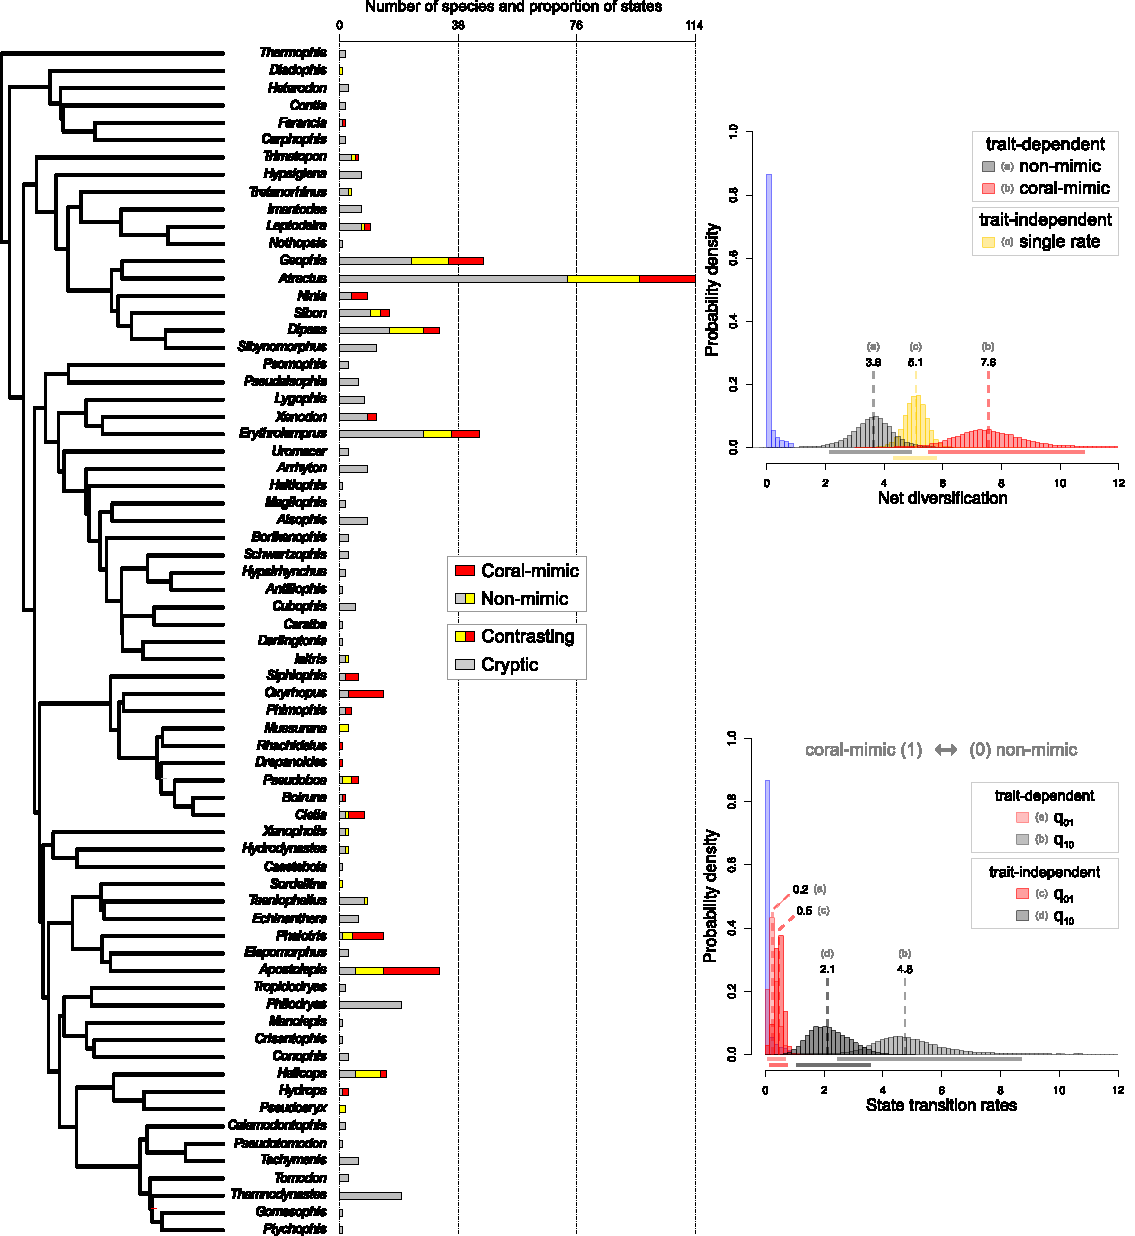
\includegraphics[scale=0.8]{Ch1_Figure_1_updated}
	\caption[Genus-level maximum clade credibility (MCC) tree of the family Dipsadidae showing the number of species assigned to each color category and posterior distribution of parameter estimates for the BiSSE model.]{Genus-level maximum clade credibility (MCC) tree of the family Dipsadidae showing the number of species assigned to each color category and posterior distribution of parameter estimates for the BiSSE model. Each color of the stacked bar chart (center) correspond to different elements of the color patterns in the group; species that do not show contrasting color patterns (i.e., cryptic coloration) are shown in gray, species with contrasting color patterns but that are not supposed mimics of coral snakes are shown in yellow, and species that show contrasting color patterns and are considered mimics of coral snakes are shown in red. (\textit{Continue on next page.})}
	\label{fig:diversity_phylo} % Figure 1.
\end{figure}

\begin{figure}[h]
  \contcaption{(\textit{Continued.}) The legend in the center of the plate applies different combinations of gray, yellow, and red to show the number of species assigned to each color category: coral-mimic (red) versus non-mimic (gray and yellow) and contrasting (yellow and red) versus cryptic (gray). Support for the genera relationships are provided in Figures \ref{fig:full_MCC1} and \ref{fig:full_MCC2}. Top-right plot shows the posterior distributions of net diversification rates under the trait-dependent (coral-mimic vs. non-mimic) and trait-independent BiSSE models. Bottom-right plot shows the posterior distributions of transition rates under the trait-dependent and trait-independent BiSSE models. Estimates are the combined posterior distribution from MCMC BiSSE runs across a pool of 100 phylogenetic trees. Prior distributions for the MCMC searches are shown in blue (unmarked distributions), the horizontal lines below each posterior distribution represent the 95\% confidence interval, and the vertical hashed lines show median values.} % Continued caption for Figure 1.
\end{figure}

\begin{figure}[h]
	\centering
	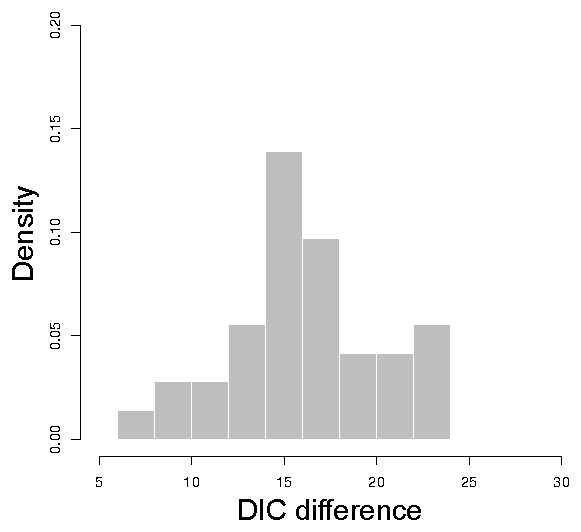
\includegraphics[scale=0.8]{Ch1_Figure_2_updated}
	\caption[Results of model selection between trait-dependent and trait-independent BiSSE models.]{Results of model selection between trait-dependent and trait-independent BiSSE models using the Bayesian Deviance Information Criteria (DIC) for the coral-mimic versus non-mimic category. Plot shows the DIC scores for the trait-dependent model (full model) subtracted from the scores for the trait-independent model (constrained model). DIC values were calculated across a pool of 100 phylogenetic trees. Large values (larger than 4 units as a rule of thumb) are expected if the trait-dependent model is to be preferred over the trait-independent model.}
	\label{fig:dic_plot} % Figure 2.
\end{figure}

\begin{figure}[h]
	\centering
	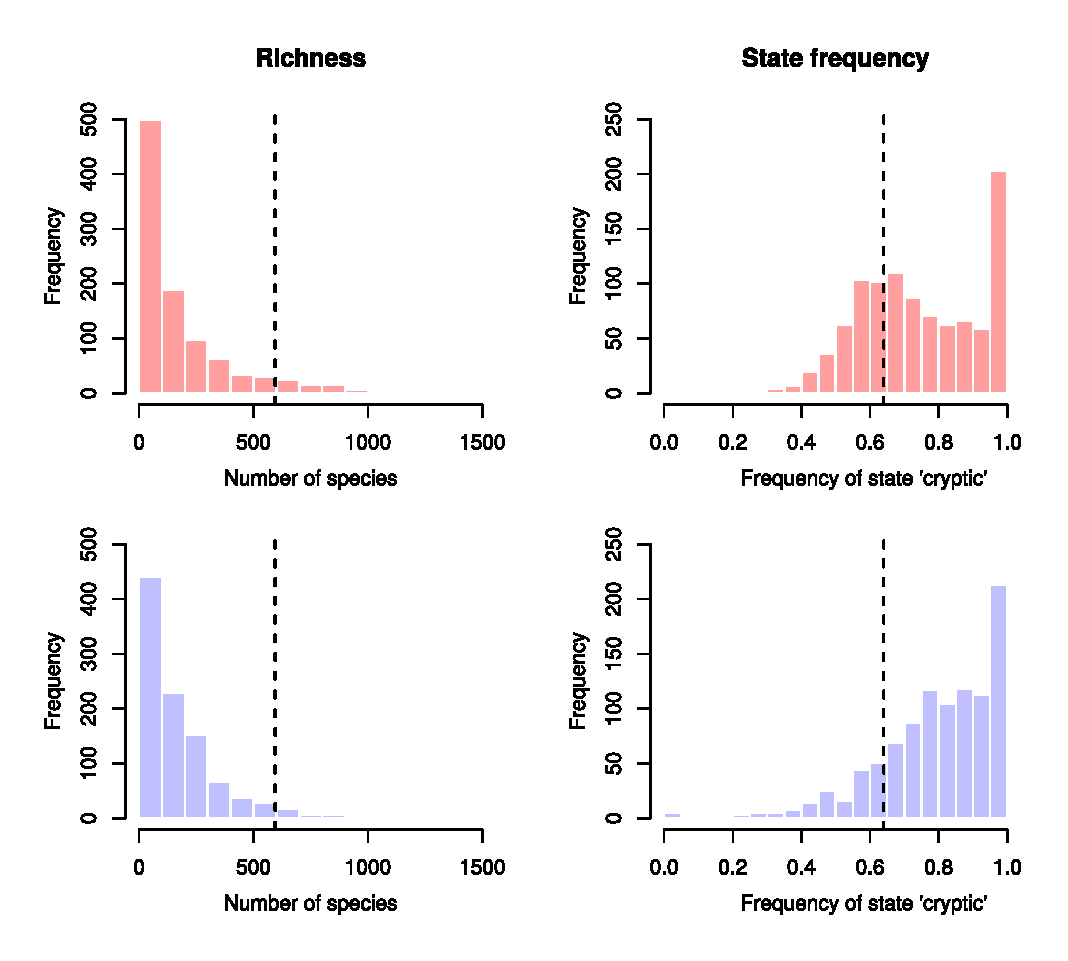
\includegraphics[scale=0.85]{Ch1_Figure_3_updated}
	\caption[Results from the posterior predictive simulations for BiSSE under the trait-dependent and the trait-independent models.]{Results from the posterior predictive simulations for BiSSE under the trait-dependent (top row - red) and the trait-independent models (bottom row - blue). Simulation parameters were drawn from the joint posterior distribution of each BiSSE model (contrasting versus cryptic color category) and phylogenetic trees. At each replicate a phylogeny was simulated under the BiSSE model until the sum of branch lengths from root to tip of the tree was equal to 1 (same as the empirical phylogeny). Left column: Total number of species in the resulting phylogenies. Vertical dashed lines show the number of species used in our analysis (594 spp.). Right column: Relative frequency of the state 0 (cryptic). Vertical dashed lines show the observed frequency of cryptic species in the data (0.64). Note that both trait-dependent and trait-independent BiSSE models show similar deviations from the observed data.}
	\label{fig:predic_BiSSE} % Figure 3.
\end{figure}

\begin{figure}[h]
	\centering
	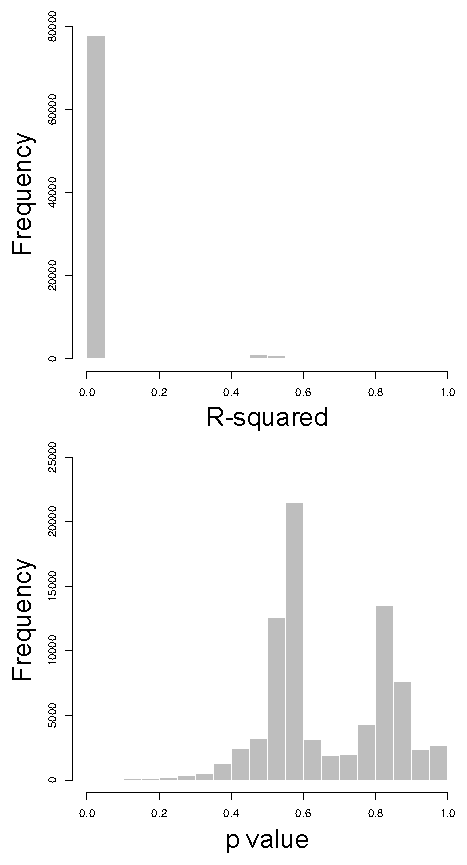
\includegraphics[scale=0.9]{Ch1_Figure_4_updated}
	\caption[Results from linear regressions between net diversification rates estimated using BAMM and the proportion of the category coral-mimic for each dipsadid genera.]{Results from linear regressions between net diversification rates estimated using BAMM (prior on expected number of shifts $\gamma$ = 1) and the proportion of the category coral-mimic for each dipsadid genera. Plots show a distribution of linear regression tests generated by repeating the analyses for each sample of the posterior distribution of the BAMM diversification estimates combined across 10 randomly sampled phylogenetic trees. Top plot shows the resulting distribution of R-squared and bottom plot the distribution of p values.}
	\label{fig:linear_BAMM} % Figure 4.
\end{figure}

\begin{figure}[h]
	\centering
	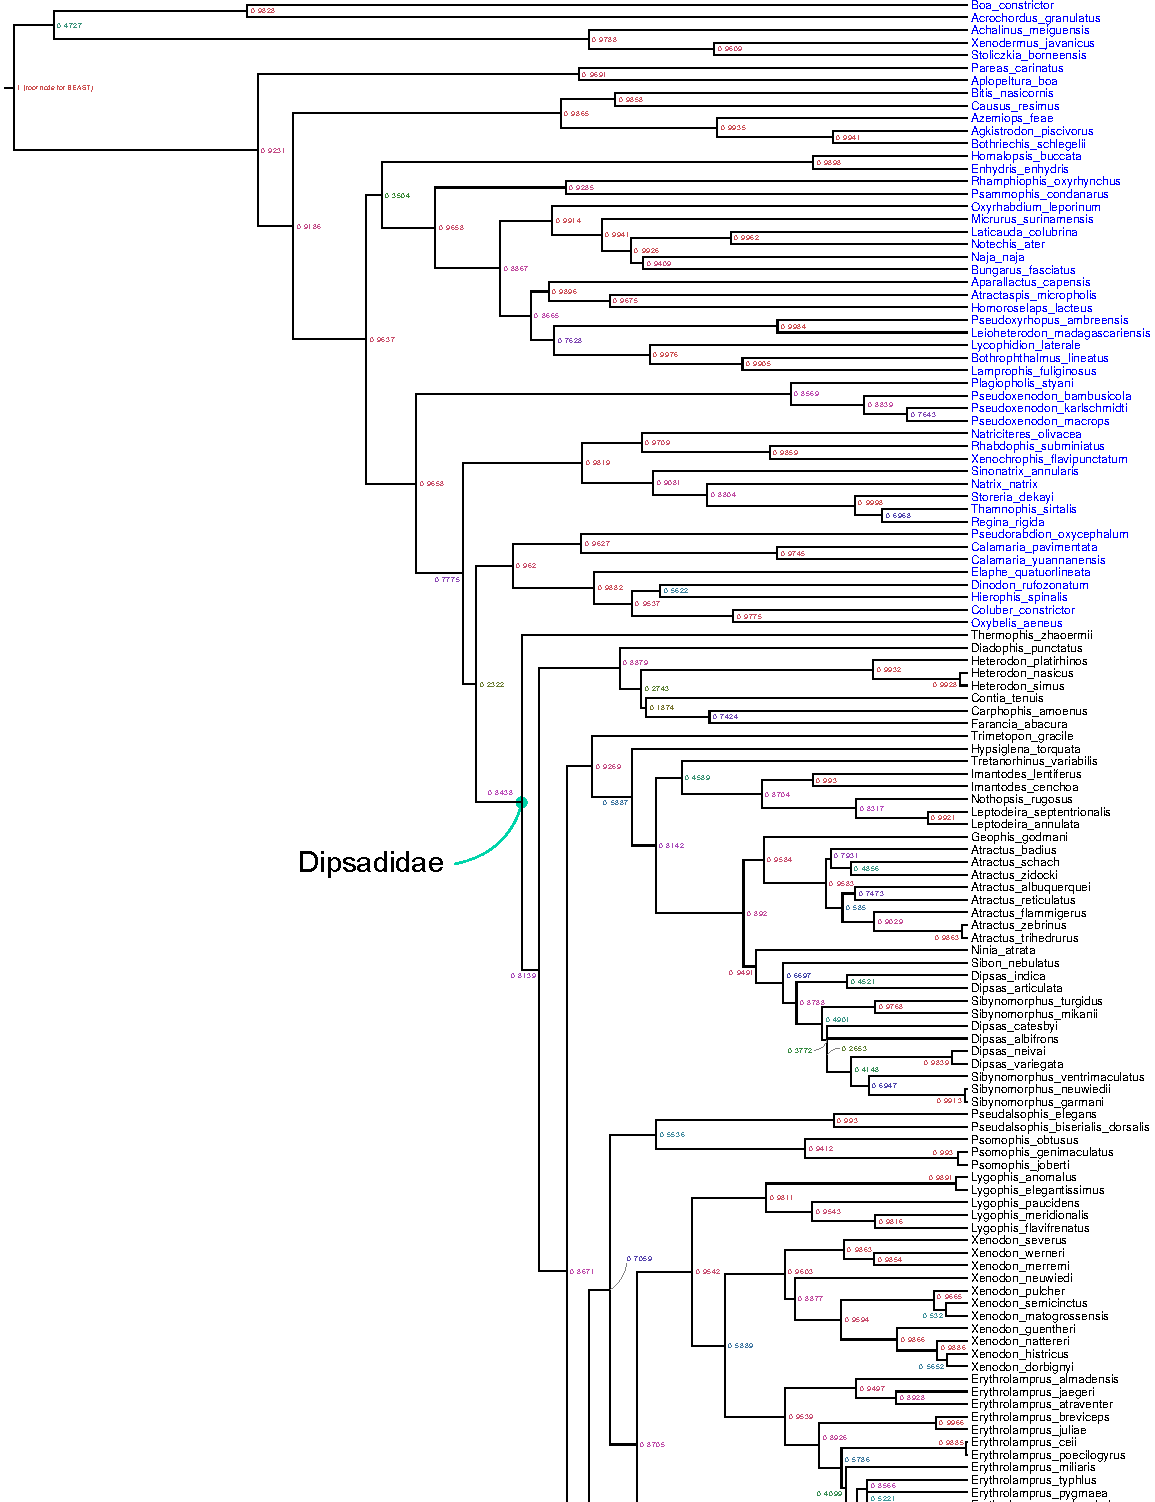
\includegraphics[scale=0.8]{Ch1_Figure_S1_updated_top}
	\caption[Maximum clade credibility tree with all species (Part 1).]{Maximum clade credibility tree with all species. Support values are posterior probabilities. Outgroup species highlighted in blue. Continues on Figure \ref{fig:full_MCC2}.}
	\label{fig:full_MCC1} % Figure S1.
\end{figure}

\begin{figure}[h]
	\centering
	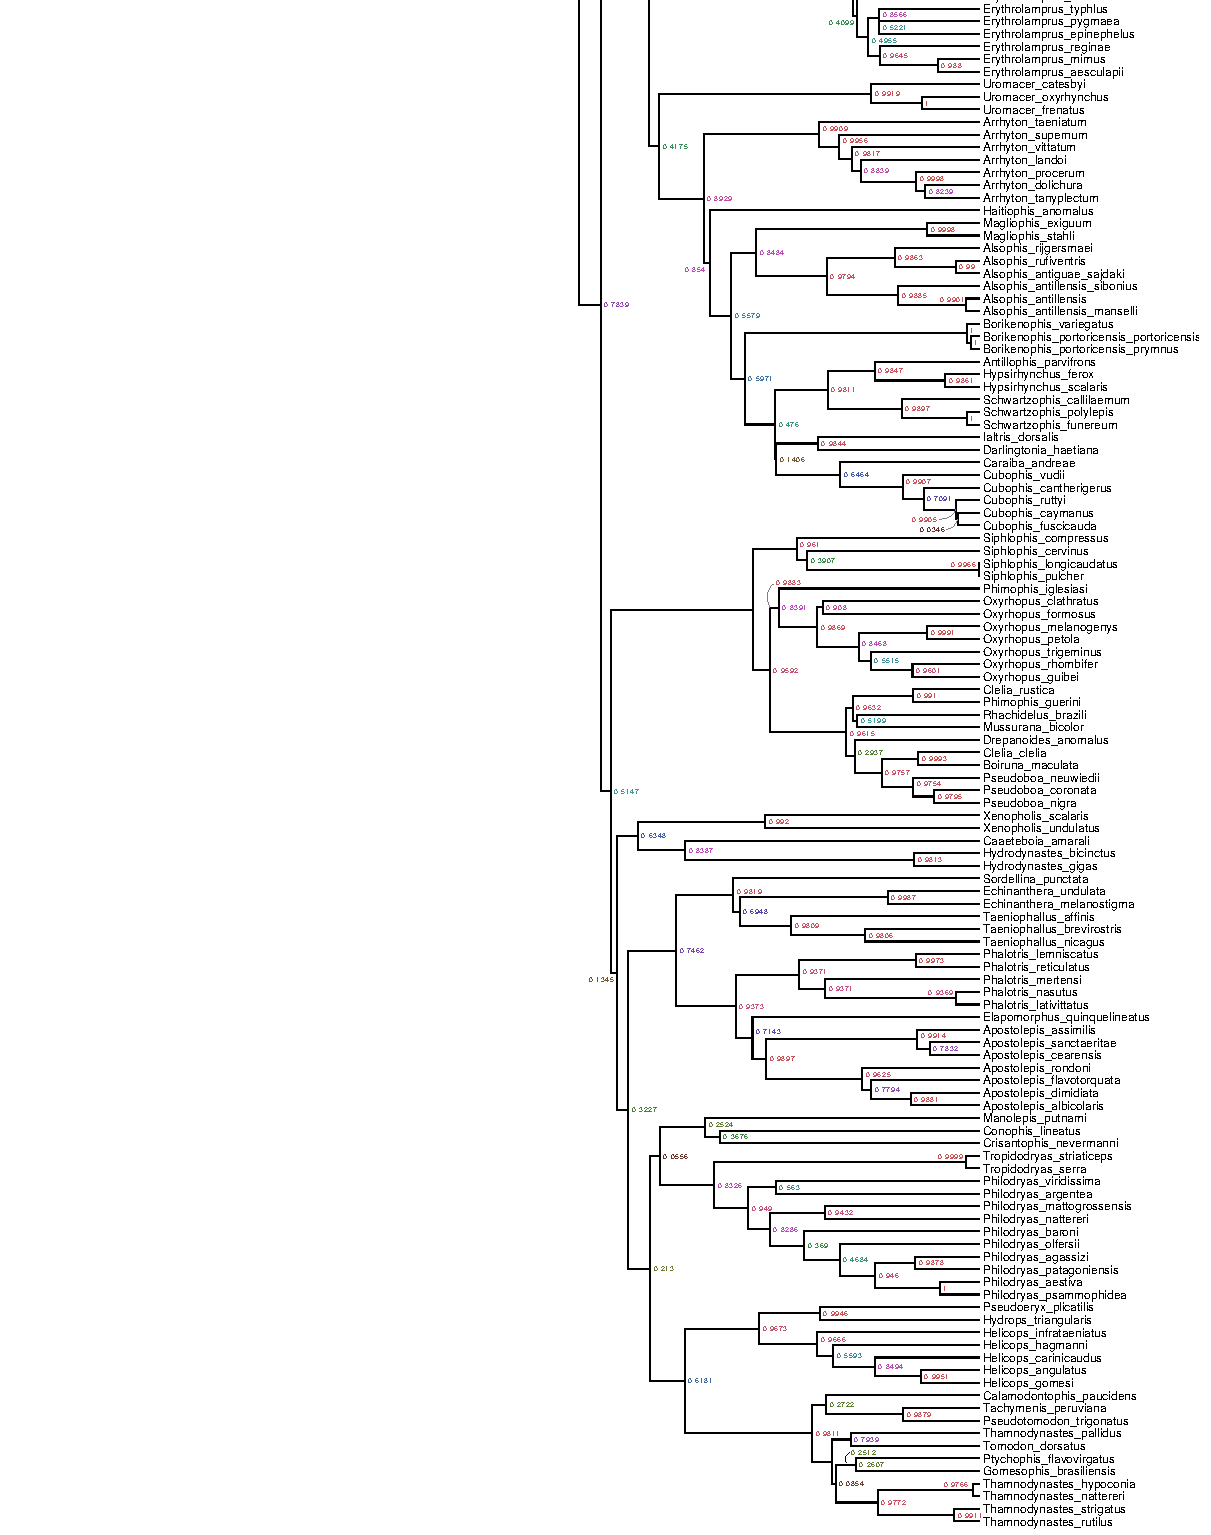
\includegraphics[scale=0.8]{Ch1_Figure_S1_updated_bottom}
	\caption[Maximum clade credibility tree with all species (Part 2).]{Maximum clade credibility tree with all species. Support values are posterior probabilities. Continuation for Figure \ref{fig:full_MCC1}.}
	\label{fig:full_MCC2} % Figure S1.
\end{figure}

\begin{figure}[h]
	\centering
	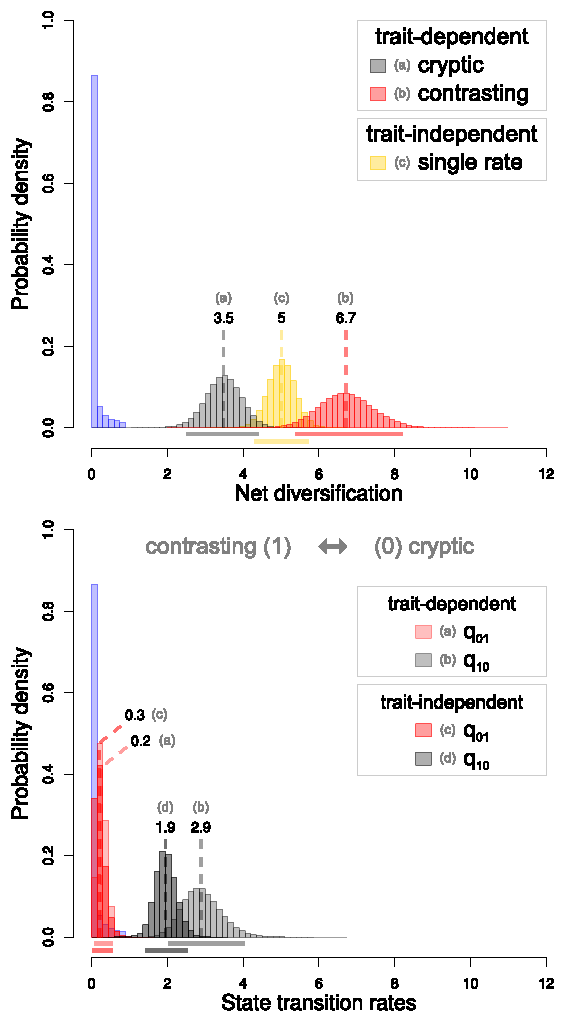
\includegraphics[scale=0.85]{Ch1_Figure_S2_updated}
	\caption[Parameter estimates for the BiSSE model under the contrasting versus cryptic color category.]{Parameter estimates for the BiSSE model under the contrasting versus cryptic color category. Top plot shows the posterior distributions of net diversification rates under the trait-dependent and trait-independent BiSSE models. Bottom plot shows the posterior distributions of transition rates under the trait-dependent and trait-independent BiSSE models. Estimates are the combined posterior distribution from MCMC BiSSE runs across a pool of 100 phylogenetic trees. Prior distributions for the MCMC searches are shown in blue (unmarked distributions), the horizontal lines below each posterior distribution represent the 95\% confidence interval, and the vertical hashed lines show median values.}
	\label{fig:par_BiSSE} % Figure S2.
\end{figure}

\begin{figure}[h]
	\centering
	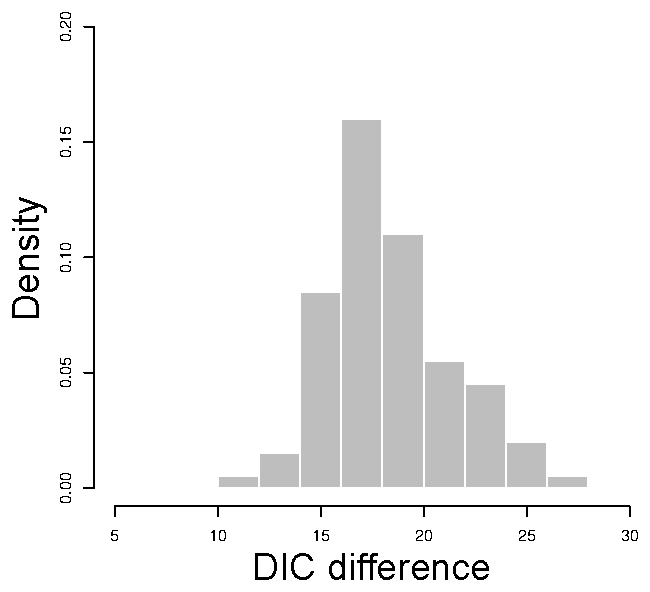
\includegraphics[scale=0.7]{Ch1_Figure_S3_updated}
	\caption[Results of model selection between trait-dependent and trait-independent BiSSE models.]{Results of model selection between trait-dependent and trait-independent BiSSE models using the Bayesian Deviance Information Criteria (DIC) for the contrasting versus cryptic category. Plot shows the DIC scores for the trait-dependent model (full model) subtracted from the scores for the trait-independent model (constrained model). DIC values were calculated across a pool of 100 phylogenetic trees. Large values (larger than 4 units as a rule of thumb) are expected if the trait-dependent model is to be preferred over the trait-independent model.}
	\label{fig:model_select} % Figure S3.
\end{figure}

\begin{figure}[h]
	\centering
	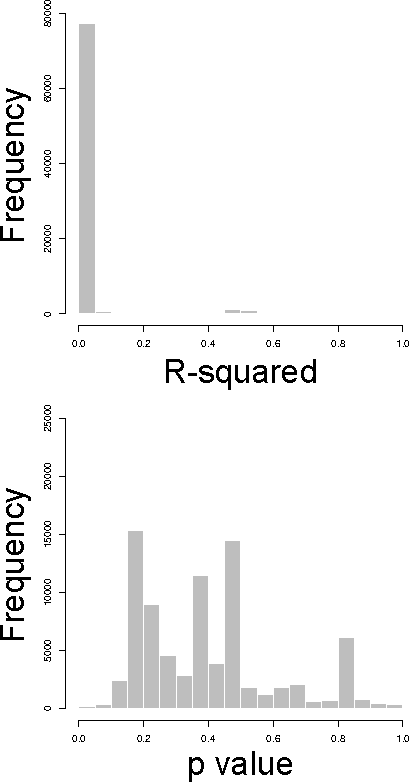
\includegraphics[scale=0.9]{Ch1_Figure_S4_updated}
	\caption[Results from linear regressions between net diversification rates estimated using BAMM.]{Results from linear regressions between net diversification rates estimated using BAMM (prior on expected number of shifts $\gamma$ = 1) and the proportion of the category contrasting for each dipsadid genera. Plots show a distribution of linear regression tests generated by repeating the analyses for each sample of the posterior distribution of the BAMM diversification estimates combined across 10 randomly sampled phylogenetic trees. Top plot shows the resulting distribution of R-squared and bottom plot the distribution of p values.}
	\label{fig:supp_linear_BAMM} % Figure S4.
\end{figure}

\begin{figure}[h]
	\centering
	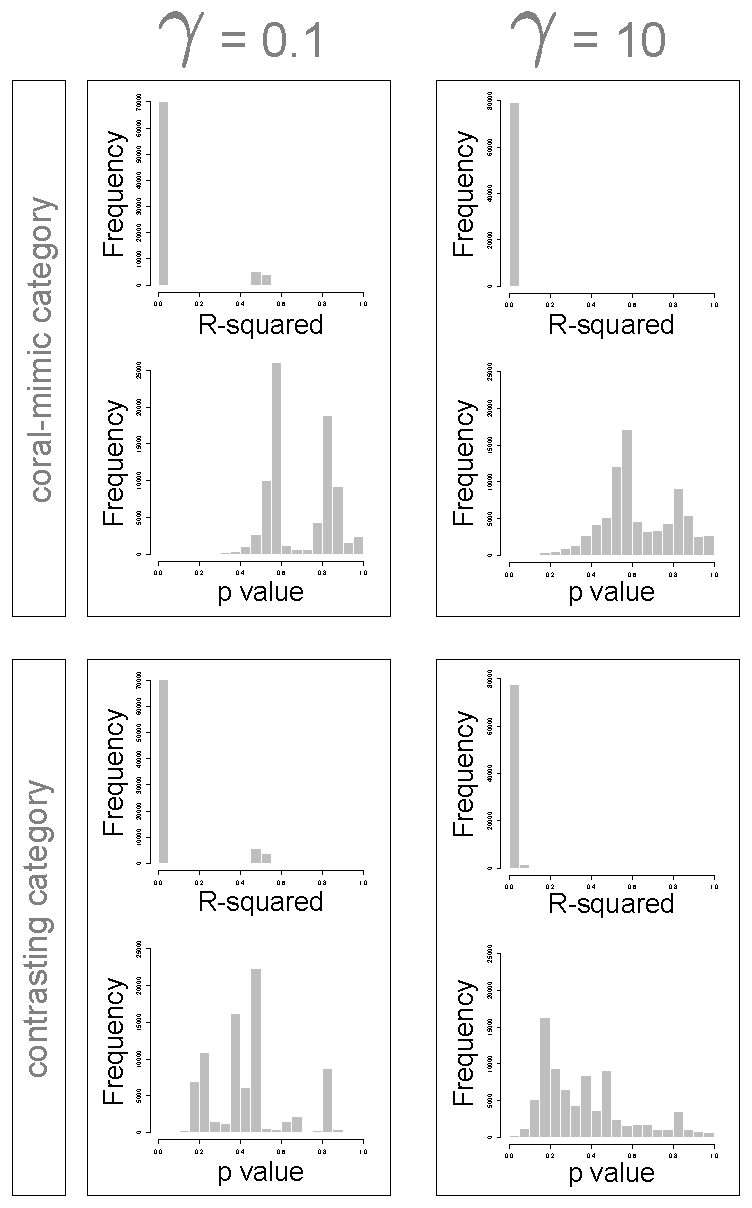
\includegraphics[scale=0.8]{Ch1_Figure_S5_updated}
	\caption[Results from linear regressions between net diversification rates estimated using BAMM and the proportion of both color categories coral-mimic and contrasting for each dipsadid genera under different prior distributions on the number of expected rate shifts.]{Results from linear regressions between net diversification rates estimated using BAMM and the proportion of both color categories coral-mimic and contrasting for each dipsadid genera under different prior distributions on the number of expected rate shifts. Each plot show a distribution of results from linear regression tests generated by repeating the analyses for each sample of the posterior distribution of BAMM diversification estimates combined across 10 randomly sampled phylogenetic trees. The top plot within each treatment show the resulting distribution of R-squared and bottom plot the distribution of p values. Top row are results using the color category coral-mimic and bottom row using category contrasting. Results on the left column were based on a prior distribution for the expected number of shifts ( $\gamma$ ) equal to 0.1 and on the right column equal to 10.}
	\label{fig:prior_linear_BAMM} % Figure S5.
\end{figure}

%% This is the start of Chapter 2.

\chapter{ESTIMATING CORRELATED RATES OF TRAIT EVOLUTION WITH UNCERTAINTY}

\section{Abstract}

Correlated evolution among traits can happen due to genetic constraints, ontogeny, and selection and have an important impact on the trajectory of phenotypic evolution. Thus, shifts in the pattern of evolutionary integration may allow the exploration of novel regions of the morphospace by lineages. Here we use phylogenetic trees to study the pace of evolution of several traits and their pattern of evolutionary correlation across clades and over time. We use regimes mapped to the branches of the phylogeny to test for shifts in evolutionary integration. Our approach incorporates the uncertainty related to phylogeny, ancestral state estimates and parameter estimates to produce posterior distributions using Bayesian Markov chain Monte Carlo. We implemented the use of summary statistics to test for regime shifts based on a series of attributes of the model that can be directly relevant to biological hypotheses. In addition, we extend Felsenstein's pruning algorithm to the case of multivariate Brownian motion models with multiple rate regimes. We performed extensive simulations to explore the performance of the method under a series of scenarios. Finally, we provide two test cases; the evolution of a novel buccal morphology in fishes of the family Centrarchidae and a shift in the trajectory of evolution of traits during the radiation of anole lizards to the Caribbean islands.

\section{Introduction}

Correlated evolution among traits, known as evolutionary integration, is ubiquitous across the tree of life and can have an important impact on the trajectory of phenotypic evolution \citep{Olson_Miller_1958, klingenberg_evolutionary_2013, armbruster_integrated_2014, klingenberg_review_2014, goswami_macroevolutionary_2014, goswami_fossil_2015, melo_modularity:_2016}. Genetic constraints, ontogeny, and selection have pivotal roles in the development and maintenance of morphological integration over time \citep{arnold_constraints_1992, arnold_adaptive_2001, pigliucci_evolvability_2004, goswami_fossil_2015, melo_modularity:_2016}. When the additive genetic covariance between traits is strong, then evolutionary correlation is likely due to genetic factors. In contrast, traits might not show strong genetic covariance and still be evolutionarily integrated due to correlated selection, which can be a result of distinct factors, such as anatomical interactions during growth or coordinated function \citep{armbruster_causes_1996, armbruster_integrated_2014}. For instance, correlated evolution can be favored by selection to maintain a cohesive pattern of variation among traits with a shared function, but evolution can be hindered if the genetic covariance is not aligned with the selection gradient \citep{lande_quantitative_1979, schluter_adaptive_1996, villmoare_morphological_2012, goswami_macroevolutionary_2014}. Alternatively, when evolutionary correlation is mainly a result of correlated selection then the morphospace occupied by lineages can be restricted by the strength and direction of the selection gradient \citep{felsenstein_phylogenies_1988, armbruster_causes_1996}. Shifts in the pattern of evolutionary integration among traits over macroevolutionary scales, due to changes in the genetic architecture or selection gradient, may play a fundamental role in the exploration of novel regions of the morphospace \citep{young_serial_2005, goswami_cranial_2006, revell_phylogenetic_2009, monteiro_adaptive_2010, hallgrimsson_generation_2012, claverie_modularity_2013}. 

Macroevolutionary transitions in morphospace evolution have been associated with both increases and decreases in the evolutionary integration among traits. In centrarchid fishes, for example, the evolution of a novel mouth morphology was followed by a rapid differentiation of feeding habits. More specifically, the increase in the evolutionary correlation between two morphological features of the suction-feeding mechanism in species of \textit{Micropterus} is associated with a specialization towards consumption of larger prey \citep{collar_comparative_2005, revell_phylogenetic_2009}. In contrast, the once strong developmental integration between the fore- and hindlimbs of early tetrapods underwent a dramatic change allowing the limbs to respond to diverging selective pressures and leading to the evolution of bipedalism and flight \citep{young_serial_2005, young_development_2010, dececchi_body_2013}. These examples show the role of shifts in evolutionary integration associated with the evolution of novel morphologies. However, stable patterns of evolutionary integration over long time scales can be responsible for the constraint of lineages to limited regions of the morphospace and might be a plausible mechanism associated with patterns of stasis observed in the fossil record \citep{pigliucci_evolvability_2004, bolstad_genetic_2014, goswami_fossil_2015}. Thus, evolutionary trait correlations are central to the maintenance of form and function through time, but can either drive or slow morphological differentiation.

Despite the prevalent role of evolutionary integration, most of what we know about the tempo and mode of trait evolution come from studies of single traits \citep[e.g.,][among others]{harmon_early_2010, hunt_simple_2015}. Even when multiple traits are the object of investigation, studies often use principal component axes \citep[or phylogenetic PCA;][]{revell_size-correction_2009} to reduce the dimensionality of the data so that univariate methods can be applied \citep[][see \citealt{uyeda_comparative_2015} for more examples]{harmon_early_2010, mahler_exceptional_2013, klingenberg_evolutionary_2013}. This is most likely a reflection of the phylogenetic comparative models of trait evolution available for use, since few are focused on two or more traits \citep[but see][]{revell_testing_2008, hohenlohe_mipod:_2008, revell_phylogenetic_2009, bartoszek_phylogenetic_2012, adams_comparing_2012, adams_quantifying_2014, Clavel_mvmorph}. However, studying one trait at a time eliminates the possibility of identifying patterns of evolutionary correlation, while principal component axes does not allow testing for evolutionary shifts in integration because the orientation of the PC axes are homogeneous across the branches of the phylogenetic tree. Furthermore, it also has been shown that PCA can influence our biological interpretation about the mode of evolution of the data \citep{uyeda_comparative_2015} because the first PC axes are consistently estimated as early bursts of differentiation whereas the last axes store a strong signal of stabilizing selection, independent of the true model of evolution of the traits. As a result, we need models that apply to multivariate data as such in order to better understand macroevolutionary patterns of evolutionary integration.

One way to model multivariate trait evolution using phylogenetic trees is through the evolutionary rate matrix \citep{hohenlohe_mipod:_2008, revell_testing_2008, revell_phylogenetic_2009, adams_assessing_2014}. This is a variance-covariance matrix that describes the rates of trait evolution under Brownian motion in the diagonals and the evolutionary covariance among traits (i.e., the pattern of evolutionary integration) in the off-diagonals \citep{huelsenbeck_detecting_2003, revell_testing_2008}. The evolutionary rate matrix is ideal for studying patterns of evolutionary integration because it allows for simultaneous estimate of the individual rates of evolution of each trait as well as the evolutionary covariance between each pair of traits. It is also a flexible model, since any number of evolutionary rate matrix regimes can be fitted to the same phylogenetic tree \citep{revell_phylogenetic_2009}. The contrast between evolutionary rate matrices independently estimated in different regions of the tree can inform us about the magnitude and direction of shifts in the pattern of evolutionary integration.

One of the challenges of working with rate matrices is that covariances can be hard to estimate, especially when the number of species (observations) is small relative to the number of traits (parameters) in the model. As the number of parameters in a model increases, the amount of data required for proper estimation also increases and it becomes crucial to directly incorporate uncertainty in parameter estimates when interpreting results. However, the majority of studies to date have relied on point estimates of the evolutionary rate matrix by maximum likelihood \citep[][but see \citealp{huelsenbeck_detecting_2003} and \citealp{dines_sexual_2014} for exceptions]{revell_testing_2008, revell_phylogenetic_2009, Clavel_mvmorph, goolsby_pseudolik_2016}. Although the confidence interval around the maximum likelihood estimate can be used as a measure of uncertainty, this quantity is rarely reported \citep{revell_testing_2008, revell_phylogenetic_2009, adams_comparing_2012, immler_distinct_2012, adams_assessing_2014, collar_biting_2014}. Furthermore, the uncertainty in parameter estimates does not take direct part in model selection using likelihood ratio tests or AIC \citep{burnham_model_2003}, which can lead researchers to erroneous conclusions about their models. Besides the possible uncertainty in parameter estimates, there is an important computational burden associated with the evaluation of the likelihood function of the multivariate Brownian motion model due to the computation of matrix inversions and determinants \citep{felsenstein_1973, hadfield_general_2010, freckleton_fast_2012}. Thus, computational time can become a limitation when performing a large number of likelihood evaluations, such as in simulation based approaches.

Recently, \citet{adams_quantifying_2014} described a method to estimate the rate of evolution under Brownian motion of traits defined by several dimensions (high-dimensional data), even when the number of trait dimensions exceeds the number of lineages in the phylogeny. This method was extended to a plethora of variations based on the same general framework \citep[][see also \citet{goolsby_pseudolik_2016} for a different implementation]{adams_assessing_2014, adams_generalized_2014, denton_new_2015}. These methods work with high-dimensional data as a result of the use of distance matrices rather than covariance matrices, since the later becomes singular if the number of variables is larger than the number of observations. However, by avoiding the calculation of the covariance among trait dimensions \citep{adams_quantifying_2014}, such suite of methods assume a homogeneous rate of evolution shared by all dimensions of a trait (the $\sigma^{2}_{mult}$). Thus, $\sigma^{2}_{mult}$ is ideal for high-dimensional traits such as shape data, but it has limitations for the study of evolutionary integration among multiple traits.

In order to ask questions about the evolution of integration using phylogenetic trees we need a computationally efficient method that can estimate evolutionary rate matrices while incorporating uncertainty in parameter estimates. Here we implement a Bayesian estimate for the evolutionary rate matrix using Markov chain Monte Carlo (MCMC) to provide a direct assessment of the uncertainty associated with parameter estimates in the form of a posterior distribution. Our implementation also allows for multiple regime configurations and/or phylogenetic trees to be incorporated in the MCMC chain, thus integrating the uncertainty associated with ancestral state estimates and phylogenetic reconstruction to the analysis. In order to increase the performance of the likelihood evaluation, we implemented Felsenstein's \citeyearpar{felsenstein_1973} pruning algorithm. We also derive a new version of the pruning algorithm that is suitable for the special case when several rate regimes of the multivariate Brownian motion model are fit to different branches of the same phylogenetic tree. We apply our new approach to two biological examples: the fast evolution of morphology associated with the radiation of \textit{Anolis} lizards from mainland South America to the Caribbean islands \citep{pinto_testing_2008, mahler_exceptional_2013, moreno-arias_patterns_2016} and the shift of feeding habits driven by the change in mouth morphology in Centrarchidae fishes \citep{revell_phylogenetic_2009}. We show that there is no detectable shift in the evolutionary integration among morphological traits during the anole radiation and that there is significant uncertainty in estimates of evolutionary correlation associated with the Centrarchidae mouth traits. We also provide results from extensive simulations showing that our approach has good performance under diverse scenarios of correlated evolution.

\section{Methods}

\subsection{A new pruning algorithm for multivariate Brownian motion with multiple regimes}

To test for shifts in the pattern of evolutionary integration among traits we need to estimate the rates of evolution for the individual traits and their evolutionary covariation, i.e. by estimating the evolutionary rate matrix \citep[$\mathbf{R}$;][]{revell_testing_2008}. \citet{revell_phylogenetic_2009} derived a general form of the likelihood function for the model that allows for several independent matrices assigned to different branches of the phylogenetic tree.

\begin{equation} \label{eq:lik_R}
L_{p} = \frac{\exp [-(\mathbf{y}-\mathbf{Da}^{T})^{T} (\sum\limits_{k=1}^{p} \mathbf{R}_{k} \otimes \mathbf{C}_{k})^ \frac{-1 (\mathbf{y}-\mathbf{Da}^{T})}{2}]}{\sqrt{(2\pi)^{nr} \mid \sum\limits_{k=1}^{p} \mathbf{R}_{k} \otimes \mathbf{C}_{k} \mid}}
\end{equation}

Where $\mathbf{y}$ is a vector of length $n \cdot r$ derived by concatenating the columns of a $n$ by $r$ matrix of trait values for $n$ tips and $r$ traits; $\mathbf{D}$ is a $n \cdot r$ by $r$ design matrix composed of 1 for each $(i,j)$ entry that satisfies $(j-1) \cdot n < i \leq j \cdot n$ and 0 otherwise; $\mathbf{a}$ is a vector with $r$ root values for the tree (or the phylogenetic mean); $\mathbf{R}_{k}$ is the $k$th evolutionary rate matrix with size $r$. Each of the $\mathbf{C}_{k}$ matrices has only the sum of branch lengths which were assigned to the respective evolutionary rate matrix. Thus, $\sum\limits_{k=1}^{p} \mathbf{C}_{k}$ is equal to the phylogenetic covariance matrix ($\mathbf{C}$) for the whole tree. The elements of $\mathbf{C}$ are composed by the sum of branch lengths shared by each pair of taxa \citep{felsenstein_1973}. Finally, $p$ is the number of $\mathbf{R}$ matrix regimes fitted to the tree. When $p$ is equal to 1, equation (\ref{eq:lik_R}) reduces to the likelihood function for a single $\mathbf{R}$ matrix \citep{revell_testing_2008}.

The likelihood function for the evolutionary rate matrix as shown requires the matrix inversion and determinant to be computed for the sum of the Kronecker product between each $\mathbf{R_{k}}$ and $\mathbf{C_{k}}$ matrices. However, the matrices resulted from this product can be very large because each $\mathbf{R}$ has dimension equal to the number of traits in the data whereas $\mathbf{C}$ is as large as the number of tips in the phylogeny. Some methods can be used to speed up the computation in the case of multiple rate regimes applied to the tree. For instance, the `rpf' method avoids the explicit computation of the matrix inversion and determinant by applying Cholesky factors \citep{Gustavson_rpf, Clavel_mvmorph} whereas \citet{goolsby_pseudolik_2016} recently introduced the use of pairwise composite likelihoods, which consists of the product of the pairwise likelihoods computed for all combinations of traits. These methods reduce the computational time for the evaluation of the likelihood but are still more time consuming than the pruning algorithm \citep{felsenstein_1973, freckleton_fast_2012, caetano_ratematrix_2017}. Here, we expand the pruning algorithm applied to the multivariate Brownian motion model \citep{felsenstein_1973, freckleton_fast_2012} to compute the likelihood even when multiple evolutionary rate matrices are fitted to different branches of the phylogenetic tree. This algorithm is implemented in the R package \texttt{ratematrix} \citep{caetano_ratematrix_2017}.

\subsection{Computing the likelihood for the multivariate Brownian motion model with multiple regimes using the new pruning algorithm}

The pruning algorithm explores the property that trait changes in each of the branches can be modelled independently and applies a multivariate normal density to compute the likelihood of evolutionary changes at each branch assuming a Brownian motion model \citep{felsenstein_inferring_2004, freckleton_fast_2012}. When multiple rate regimes are fitted to a phylogeny, the likelihood is often computed by scaling the branch lengths by the rates \citep[e.g.,][]{Eastman_2011}. However, this procedure is not applicable to the multivariate case, since the product of the length of a branch and the BM rate is a matrix. We derived the pruning algorithm for multiple rate regimes by following the same procedures described by \citet{felsenstein_1973, felsenstein_inferring_2004}, but assuming that all rates are multivariate, that rates are different at each branch and that branches can have more than one rate regime \citep[after][]{revell_phylogenetic_2009}. This algorithm completely avoids the calculation of the matrix inverse and the determinant of the phylogenetic covariance matrix ($\mathbf{C}$) or the Kronecker product between $\mathbf{R}$ and $\mathbf{C}$ matrices. However, the inverse of the $\mathbf{R}$ matrix, which will have dimensions equal to the number of traits in the data set, is still required.

In this extension of the algorithm, each branch of the phylogeny can be assigned to one or more evolutionary rate matrix ($\mathbf{R}$) regimes and the sum of the portions of the branch assigned to each regime need to be equal to the total length of that branch \citep{revell_phylogenetic_2009}. We demonstrate that the algorithm yields the same likelihood as in \citet{felsenstein_1973} and \citet{freckleton_fast_2012} by showing that all calculations converge when a single regime is fitted to tree. The pruning algorithm works by visiting the tips and going down node by node. At each step the contrast between two tips is computed and a new ``phenotype" value replaces the two original tips, becoming the new tip. The likelihood of the contrast is calculated and we move to the next contrast until we reach the root node. From here on we will refer to Figure \ref{fig:example_phylo} as an example of phylogenetic tree. Where $\mathbf{x}_{i}$ is a vector with $r$ trait values for tip $i$ and $v_{i}$ is the branch length leading to tip or node $i$. We will refer to the node representing the common ancestor of tips 1 and 2 as the node 4 and the node representing the common ancestor of all tips as the root node. The method works as following:

\begin{enumerate}

\item \textbf{Calculate the contrast.} Choose a pair of tips $i$ and $j$ with a unique and exclusive common ancestor $k$. In our example, the selected species are 1 and 2. Compute the contrast $\mathbf{u}_{ij} = \mathbf{x}_{i} - \mathbf{x}_{j}$.

\item \textbf{Compute the log-likelihood.} Use the vector of contrasts ($\mathbf{u}_{ij}$), the number of traits in the data ($r$), the branch lengths ($v_{i}$ and $v_{j}$), and the length of the branches assigned to each of the $k$ evolutionary rate matrix regimes \citep{revell_phylogenetic_2009} to compute the log-likelihood:
\begin{equation} \label{eq:app_lik}
\begin{split}
& L = - \frac{1}{2} \left( \: r \log(2 \pi) + \log | \mathbf{S_{i}} + \mathbf{S_{j}}  | + \mathbf{u}_{ij}^\intercal \: (\mathbf{S_{i}}+\mathbf{S_{j}})^{-1} \:  \mathbf{u}_{ij} \: \right)  \\
\text{where} & \\
& \mathbf{S_{i}} = \mathbf{R_{1}} \: v_{1i} + \mathbf{R_{2}} \: v_{2i} + \ldots + \mathbf{R_{k}} \: v_{ki} \\
& \mathbf{S_{j}} = \mathbf{R_{1}} \: v_{1j} + \mathbf{R_{2}} \: v_{2j} + \ldots + \mathbf{R_{k}} \: v_{kj} \\
\text{and} & \\
& v_{i} = v_{1i} + v_{2i} + \ldots + v_{ki} \\
& v_{j} = v_{1j} + v_{2j} + \ldots + v_{kj}
\end{split}
\end{equation}

If we assume a single evolutionary rate matrix is fitted to the whole tree, equation \ref{eq:app_lik} reduces to equation 10 in \citet{freckleton_fast_2012}:
\begin{equation*}
\begin{split}
\text{Let} &\\
&\mathbf{R} = \mathbf{R_{1}} = \mathbf{R_{2}} = \ldots = \mathbf{R_{k}} \\
\text{then} &\\
\mathbf{S_{i}} &= \mathbf{R_{1}} \: v_{1i} + \mathbf{R_{2}} \: v_{2i} + \ldots + \mathbf{R_{k}} \: v_{ki} \\
&=  \mathbf{R} \: v_{1i} + \mathbf{R} \: v_{2i} + \ldots + \mathbf{R} \: v_{ki} \\
&= \mathbf{R} \sum_{l = 1}^{k} v_{li}
\end{split}
\end{equation*}

We know, from equation \ref{eq:app_lik}, that the sum of the portions of the branch length assigned to each regime is equal to the total length of the branch. Then:
\begin{equation*}
\begin{split}
& \mathbf{S_{i}} = \mathbf{R} v_{i} \: \: \: \: \: \text{as well as} \: \: \: \: \: \mathbf{S_{j}} = \mathbf{R} v_{j} \\
\text{and} &\\
& \mathbf{S_{i}} + \mathbf{S_{j}} = \mathbf{R} ( v_{i} + v_{j} )
\end{split}
\end{equation*}

Substituting into equation \ref{eq:app_lik}, we have:
\begin{equation} \label{eq:app_lik_proof}
\begin{split}
L &= - \frac{1}{2} \left( \: r \log(2 \pi) + \log | \mathbf{R} ( v_{i} + v_{j} )  | + \mathbf{u}_{ij}^\intercal \: (\mathbf{R} ( v_{i} + v_{j} ))^{-1} \:  \mathbf{u}_{ij} \: \right)  \\
&= - \frac{1}{2} \left( \: r \log(2 \pi) + \log | \mathbf{R} | + r \log( v_{i} + v_{j} ) + \frac{\mathbf{u}_{ij}^\intercal \: (\mathbf{R})^{-1} \:  \mathbf{u}_{ij}}{( v_{i} + v_{j} )} \: \right)  \\
\end{split}
\end{equation}
Which is the same as equation 10 in \citet{freckleton_fast_2012}\footnote{Note that the published equation in \citet{freckleton_fast_2012} has a printing error. The corrected form is \linebreak $ L = - \frac{1}{2} \left( k \log(2\pi) + \log | \mathbf{C} | + k \log \mathit{V}_{i} + \frac{\mathbf{u}_{i}^{t} \mathbf{C}^{-1} \mathbf{u}_{i}}{\mathit{V}_{i}} \right) $. The correct form can be appreciated in the function `clikGeneral' on line 393 of the Supporting Information file \texttt{MEE3\_220\_sm\_demo.R} available online \citep{freckleton_fast_2012}.}.

\item \textbf{Calculate the new phenotype vector $\mathbf{x}_{n}$ for the node $n$.} This quantity is originally calculated as the weighted average of the vector of species means for species $i$ and $j$ with weights equal to the length of the branches $v_{i}$ and $v_{j}$. For the case of a single trait, $\mathbf{x}_{1i}$ and $\mathbf{x}_{1j}$, we would have:
\begin{equation} \label{eq:app_xk_origin}
\mathbf{x}_{1n} = \frac{v_{i} \: \sigma_{1i}^{2}}{v_{i} \: \sigma_{1i}^{2} + v_{j} \: \sigma_{1j}^{2} } \: \mathbf{x}_{1j} + \frac{v_{j} \: \sigma_{1j}^{2} }{v_{i} \: \sigma_{1i}^{2} + v_{j} \: \sigma_{1j}^{2}} \: \mathbf{x}_{1i}
\end{equation}
When $\sigma_{i}^{2} = \sigma_{j}^{2}$, equation \ref{eq:app_xk_origin} becomes equivalent to equation 7 in \citet{felsenstein_1973} and the rates of each branch can be omitted. However, here we assume that rates are different in every branch, that the evolutionary covariance among traits are non-zero and that more than one rate regime can be assigned to the same branch. As a result, the rates need to be represented as variance-covariance matrices ($ \mathbf{R_1}, \mathbf{R_2}, \ldots, \mathbf{R_k} $) and the sum of the product between the portions of each branch and their rate regimes is given by the matrices $ \mathbf{S_{i}} $ and $\mathbf{S_{j}}$ (see equation \ref{eq:app_lik}). By expanding equation \ref{eq:app_xk_origin}, we have:
\begin{equation} \label{eq:app_xk_mult}
\mathbf{x}_{n} = \mathbf{S_{i}} \: ( \mathbf{S_{i}} + \mathbf{S_{j}} )^{-1} \: \mathbf{x}_{j} + \mathbf{S_{j}} \: ( \mathbf{S_{i}} + \mathbf{S_{j}} )^{-1} \: \mathbf{x}_{i}
\end{equation}

\pagebreak

In the first step of our example, we calculate the phenotype value for the node 4 ($\mathbf{x}_{4}$). Then, we prune the tips 1 and 2 from the tree, leaving only the tip 3 and the new tip 4 with vector of trait values $\mathbf{x}_{4}$. The next contrast will be calculated between $\mathbf{x}_{4}$ and $\mathbf{x}_{3}$.

\item \textbf{Compute the variance of $\mathbf{x}_{n}$.} After computing the vector of trait values for the node $n$, we need to calculate the variance associated with the uncertainty in the estimation of $\mathbf{x}_{n}$. This uncertainty is added to the variance of the branch immediately bellow the node $n$. For a single trait and we would have:
\begin{equation} \label{eq:var_to_add}
var[\mathbf{x}_{1n}] = \frac{v_{i} \sigma^{2}_{1i} \: v_{j} \sigma^{2}_{1j}}{v_{i} \sigma^{2}_{1i} + v_{j} \sigma^{2}_{1j}} + v_{n} \sigma^{2}_{1n}
\end{equation}
Where $m, \ldots, n$ are the indexes for the branches that connect the root to the node $n$ of the tree. Again, when a single rate regime is fitted to the tree, equation \ref{eq:var_to_add} is equivalent to equation 9 in \citet{felsenstein_1973}.  For the multivariate case, this quantity becomes a variance-covariance matrix which is added to $\mathbf{S_{n}}$ (the branch length below the node $n$ multiplied by the rate regimes; see equation \ref{eq:app_lik_proof}) and can be calculated as:
\begin{equation}\label{eq:var_to_add_mat}
var[\mathbf{x}_{n}] = \left( (\mathbf{S_{i}})^{-1} + (\mathbf{S_{j}})^{-1} \right)^{-1} + \mathbf{S_{n}}
\end{equation}
The equivalence between equations \ref{eq:var_to_add} and \ref{eq:var_to_add_mat} can be easily verified by checking the computation of the harmonic mean of matrices. For two scalar quantities the harmonic mean is given by $\frac{2 \: a \: b}{a+b } $ whereas for matrices we have $ \left( (\mathbf{A})^{-1} + (\mathbf{B})^{-1} \right)^{-1} $.

\item \textbf{Repeat.} Steps 1 to 4 are repeated until only two tips remains. The root node will have a zero contrast. The variance associated with the root node is computed as:
\begin{equation}
var[\mathbf{root}] = \left( (\mathbf{S_{i}})^{-1} + (\mathbf{S_{j}})^{-1} \right)^{-1}
\end{equation}

\item \textbf{Compute the final log-likelihood.} The final log-likelihood conditioned on the phylogenetic tree, rate regime and trait data is computed as the sum of all partial (node-by-node) log-likelihoods computed in step 2.

\end{enumerate}

\subsection{MCMC prior densities and sampling strategy}

We have developed and implemented a Bayesian method to estimate one or more evolutionary rate matrices from phylogenetic comparative data. Our primary objective is to provide a framework to incorporate uncertainty in the estimates of $\mathbf{R}$ as well as to build a flexible model to study shifts in evolutionary integration across clades and over time. Our method requires a phylogenetic tree with branch lengths, continuous data for two or more traits for each tip species, and it uses Metropolis-Hastings Markov chain Monte Carlo \citep[MCMC,][]{metropolis_equation_1953, hastings_monte_1970}.

We model the prior density for the vector of root values ($\mathbf{a}$) as an uniform or normal distribution and we use an uniform sliding window proposal density to sample the root value for every trait simultaneously. In contrast, the prior density and sampling scheme for the evolutionary rate matrix requires more elaboration because variance-covariance matrices are positive definite and are relatively hard to be estimated. We model $\mathbf{R}$ with two independent distributions; one for the vector of standard deviations and another for the correlation matrix \citep{barnard_modeling_2000, zhang_sampling_2006}. This method allows the prior density for the rates (vector of standard deviations) to be parametrized independently of the evolutionary integration (correlation matrix). Under this parametrization, one can assign any distribution of positive real values to the vector of standard deviations (here we use an uniform or a exponential density) and the correlation matrix is modelled as the Cholesky decomposition of variance-covariance matrices sampled from an inverse-Wishart distribution \citep{zhang_sampling_2006}. This parameter extension approach is named `separation-strategy' \citep{barnard_modeling_2000, zhang_sampling_2006} because it relies on the independent modelling of the vector of standard deviations and the correlation matrix that together compose the evolutionary rate matrix. The advantage of the separation-strategy is twofold; it allows for intuitive modelling of rates of evolution and evolutionary integration and it is an efficient proposal scheme, because matrices are guaranteed to be positive definite at every draw \citep{barnard_modeling_2000, zhang_sampling_2006}.

\subsection{Incorporating uncertainty in regime configurations and phylogenetic trees}

Our approach can integrate any number of evolutionary rate matrix regimes fitted to the same phylogenetic tree. A regime is often dictated by some categorical data which states are hypothesized to be associated with shifts in the tempo and mode of evolution of the traits under study. Regimes are often `painted' to the phylogenetic tree using stochastic mapping simulations \citep{huelsenbeck_stochastic_2003} and analyses are repeated over a sample of stochastic maps. In order to facilitate incorporation of uncertainty in both ancestral state estimates and phylogenetic inference, such as multiple phylogenetic trees sampled from a posterior distribution, we implemented a MCMC that integrates over multiple rate regime configurations and/or phylogenetic trees. At each step of the MCMC chain one phylogenetic tree is randomly sampled from a pre-determined pool of trees and used to evaluate the likelihood of the model. The approach assumes that each phylogeny or regime configuration in the pool has equal chance to be sampled, but one can also assign the frequency of sampling as a result of a previous analysis. This pool is assumed to be gathered \textit{a priori}, as a result of stochastic mapping simulations, samples from a posterior distribution of trees or other similar analyses. Although this method does incorporate the uncertainty related to alternative regime configurations, different topologies and set of branch lengths, it is not a joint estimation of the tree and the model because the MCMC only applies proposal steps to the vector of root values and the evolutionary rate matrices. 

\subsection{Testing for shifts between rate regimes}

A useful criterion to perform model selection in a Bayesian framework is the Bayes factor \citep{kass_bayes_1995}, which is a ratio between the marginal likelihoods of the competing models. However, the estimation of marginal likelihoods is a computationally expensive and contentious task. One of the most accurate methods to estimate the marginal likelihood is the stepping stone approach. This method consists of taking samples from a series of weighted posterior distributions by scaling the likelihood of the model so that a continuum between the prior and the posterior is created \citep{fan_choosing_2011, xie_improving_2011, Uyeda_BayOU}. However, the stepping stone method adds significantly to the computation burden of the analysis, because each step of the continuum represents a complete MCMC chain and a large number of steps are required to produce a sufficient approximation of the marginal likelihood \citep{Uyeda_BayOU}.

Here, we do not use Bayes factor to compare models, although implementation is feasible for future work. We focus our interpretation of results on the distribution of posterior parameter estimates, and quantify the amount of uncertainty and the magnitude of the difference between components of the evolutionary rate matrices fitted to different regimes of the tree. We implemented summary statistics that provide a framework to decide whether there is enough signal in the data to support a model comprised by multiple $\mathbf{R}$ matrix regimes. First we check the difference between untransformed $\mathbf{R}$ matrices (ss-overall), then we contrast the vector of standard deviations (ss-rates) and the difference between correlation matrices (ss-correlation) derived from these $\mathbf{R}$ matrices. The first quantity check for overall changes in the evolutionary rate matrix whereas the later two quantities check for a shift in the rates of evolution of each individual trait and the structure of evolutionary integration among traits. We perform tests by calculating the percentile of the 0 value with respect to the distribution of the difference between summary statistics computed from the joint posterior distribution of parameter estimates. If the 0 value is within 95\% of the density, then there is significant overlap between the posterior distribution of the corresponding parameter estimates and we cannot reject that the rate regimes are likely samples from the same distribution.

The approach using summary statistics described here is justified by the fact that the models are nested. This means that it is possible to collapse the posterior distribution of evolutionary rate matrices fitted to different regions of the same phylogenetic tree to produce a single distribution if enough overlap is detected.  For example, a model with three evolutionary rate matrix regimes can be reduced into a model with two regimes and so on. Thus, the summary statistics tests help us decide whether the posterior distribution between two parameters show enough overlap to justify their collapse into a single one. This argument extends to different attributes of the $\mathbf{R}$ matrix, such that one can collapse the rates of evolution of the traits into a single regime while accepting a shift in the pattern of evolutionary correlation among traits.

\subsection{Simulation study}

We performed simulations to test the performance of our Bayesian MCMC estimates and the use of summary statistics under different scenarios of correlated and uncorrelated evolution. For each simulation we used rejection sampling to generate a phylogenetic tree with 200 tips and at least one monophyletic clade containing 50 tips under a birth-death model. Then, we simulated data using a multivariate Brownian motion model for three continuous traits with two evolutionary rate matrix regimes, one for the 50 tips clade and another for the background group (Fig. \ref{fig:phylogeny_sims}). We performed four simulation scenarios: no shift (equal matrices), shift of orientation (positive versus negative evolutionary correlations), shift of rates (same evolutionary correlation but varying rates of evolution), and shift of integration (same rates but different degrees of evolutionary correlation). We applied two treatments for the scenario of shift of rates and shift of integration by varying the magnitude of the shifts. Figure \ref{fig:posterior_sims} shows the total number of simulation treatments and their true parameter values.

For all simulations we used a uniform prior for the vector of standard deviations, a marginally uniform prior for the correlation matrix \citep{barnard_modeling_2000}, and a multivariate normal prior for the vector of phylogenetic means centered in the mean of the tip data for each trait and with standard deviation equal to two times the standard deviation of the tip data (Fig. \ref{fig:prior}). We chose an informative prior for the phylogenetic mean in order to facilitate the convergence of the MCMC chains, since the root values are not the primary focus of this set of simulations. Nevertheless, we repeated a subset of the simulations using a uninformative prior assigned to the root values to show that the MCMC also performs well under this scenario. For each simulation treatment we performed 100 replicates, each replicate composed by two independent MCMC chains of 500,000 generations. The initial state of every MCMC chain was set to a random draw from its prior distribution. We checked for convergence using the \citet{gelman_R_1992} test applied to each parameter of the model (each element of the root values, standard deviation vector, and correlation matrix was considered a separate parameter). We plotted the distribution of the percentiles of the true parameter values for the simulations compared to the posterior distributions to show the proportion of MCMC estimates that contained the true value of the simulation within the 95\% highest probability density (HPD) interval. We simulated phylogenies, traits and mapped regimes using the R package \texttt{phytools} \citep{revell_phytools:_2012} and performed all parameter estimates with the package \texttt{ratematrix} \citep{caetano_ratematrix_2017}.

In order to check for congruence between our approach and maximum likelihood estimators, we used the R package \texttt{mvMORPH} \citep{Clavel_mvmorph} to find the best model using likelihood ratio tests (one regime versus two regimes) for all simulated scenarios. We compared the results from the MCMC with the maximum likelihood estimates by calculating the percentile of the MLE estimates for the two regimes model with respect to the posterior distributions and checked whether the model favored by the likelihood ratio test also showed support when relying on the summary statistics computed from the posterior distribution of parameter estimates. The comparison between the likelihood ratio test and our posterior check approach is not a formal evaluation of model test performance, since the two approaches are fundamentally distinct. On the other hand, this serve as a pragmatic comparison to show whether we can adopt the use of summary statistics calculated from the posterior distribution to make reliable choices between models with direct incorporation of uncertainty in parameter estimates while retaining the explanation power of a more formal model testing approach.

\subsection{Empirical examples}

We use two examples to show the performance of the approach with empirical datasets and to further explore the impact of the direct incorporation of uncertainty in parameter estimates and model comparison. The first example tests for a shift in the evolutionary integration among anoles traits during the Caribbean radiation. Then, we repeat the analysis from \citet{revell_phylogenetic_2009} study on the evolution of buccal traits in Centrarchidae fishes. 

Anoles are small lizards that live primarily in the tropics. There are nearly 400 anole species with diverse morphology and they have become a model system for studies of adaptive radiation and convergence \citep[][and references therein]{losos_lizards_2009, mahler_exceptional_2013}. The ancestral distribution of the genus is in Central and South America and the history of the clade includes island dispersion and radiation as well as dispersal back to the mainland \citep{nicholson_mainland_2005, losos_lizards_2009}. The adaptive radiation of anoles to the Caribbean islands and the repeated evolution of ecomorphs are the main focus of evolutionary studies in the genus \citep{mahler_ecological_2010, losos_lizards_2009, mahler_exceptional_2013}. However, mainland anoles are distributed from the north of South America to the south of North America and show more species (60\% of all species) than island anoles and equally impressive morphological diversity \citep{losos_lizards_2009}. Mainland and island anole species form distinct morphological clusters \citep{pinto_testing_2008, schaad_patterns_2010, moreno-arias_patterns_2016}, but rates of trait evolution have been shown not to be consistently different \citep{pinto_testing_2008}. Island ecomorphs can be readily distinguished by body size and the morphology of limbs, head and tail \citep{losos_lizards_2009, mahler_exceptional_2013}. Thus, it is plausible that a shift in the structure of evolutionary integration among those traits associated with the radiation to the islands played an important role on the exploration of novel regions of the morphospace and allowed the repeated evolution of specialized morphologies. Herein we test this hypothesis by fitting two evolutionary rate matrix regimes, one for mainland and other for island anole lineages.

We compiled data for snout-vent length (SVL), tail length (TL), and head length (HL) of 125 anole species (99 Caribbean and 26 mainland species) made available by \citet{mahler_exceptional_2013} and \citet{moreno-arias_patterns_2016}. We chose this set of traits because they are important for niche partitioning among anoles \citep{pinto_testing_2008, losos_lizards_2009, mahler_exceptional_2013} and also provided the best species coverage given the data currently available. We use \citet{gamble_anolis_2014} maximum clade credibility tree for all comparative analyses, but we trimmed the phylogeny to include only the species that we have morphological data. To map the different $\mathbf{R}$ matrix regimes to the phylogenetic tree we classified species as `island' or `mainland' and used the package \texttt{`phytools'} \citep{revell_phytools:_2012} to estimate the transition rates between the states in both directions using an unconstrained model (e.g., the `all rates different' model) and to perform 100 stochastic mapping simulations. We set the model to estimate one $\mathbf{R}$ matrix for each mapped state (`island' or `mainland') and we used the pool of 100 stochastic maps in the MCMC to take into account the uncertainty associated with ancestral state estimation. We ran four independent MCMC chains of 2 million generations each and used a random sample from the prior as the starting point of each chain. We set a uniform prior for the phylogenetic mean, a marginally uniform prior on the correlation matrices and a uniform prior on the vector of standard deviations for the $\mathbf{R}$ matrices. We discarded 25\% of each MCMC chain as burn-in and checked for convergence using the potential scale reduction factor \citep{gelman_R_1992}. In order to test the influence of the root state for the rate regimes, we repeated the analyses by setting the root state for the stochastic mapping simulations as a random sample between `island' and `mainland' and with the ancestral distribution fixed as `mainland'.

In addition to the analyses of mainland and island anoles lizards, we replicated the study by \citet{revell_phylogenetic_2009} as an exercise to contrast the inference of evolutionary rate matrices in the presence of a direct estimate of uncertainty provided by the posterior densities. \citet{revell_phylogenetic_2009} showed that the evolution of a specialized piscivorous diet in fishes of the genus \textit{Micropterus} is associated with a shift towards a stronger evolutionary correlation between buccal length and gape width (see Fig. 1 in \citealp{revell_phylogenetic_2009}). This tighter integration might have allowed \textit{Micropterus} lineages to evolve better suction feeding performance. For this analysis we used the same data and phylogenetic tree made available by the authors. We set prior distributions using the same approach for the analysis of anole lizards described above. We also ran four MCMC chains starting from random draws from the prior for 1 million generations and checked for convergence using the potential scale reduction factor \citep{gelman_R_1992}.

We provided scripts to reproduce simulations and analyses of the empirical data as Supplementary Material.

\section{Results}

\subsection{Performance of the method}

We ran a total of 1,200 Markov chain Monte Carlo chains to check the performance of the model under six different scenarios of correlated evolution among traits. All chains finished without errors, showed good convergence after 500,000 generations and results were congruent both with the true simulation parameters and with maximum likelihood estimates (Table \ref{tab:model_test} and Fig. \ref{fig:quantiles}). Figures \ref{fig:posterior_sims} and \ref{fig:sup_root_sims} show examples of the posterior distribution of evolutionary rate matrices and root values for each simulation scenario. Changing the prior distribution for the vector of root values from multivariate normal to uniform showed no detectable bias in the posterior distribution, however the MCMC required approximately twice as many iterations to converge (Fig. \ref{fig:sup_root_sims_flat}). The distribution of percentiles for both the MLE and the true value for the simulations with respect to the posterior distribution of parameter estimates were, on average, within the 95\% highest posterior density interval (Fig. \ref{fig:quantiles}). The likelihood ratio tests supported the two rates model about as often as our test based on summary statistics across all simulation scenarios (Table \ref{tab:model_test}). When data was simulated with a single evolutionary rate matrix across the tree but tested for two regimes, both the likelihood ratio tests and the summary statistics (ss-overall) resulted in less than 5\% of the 100 replicates with support for the wrong model.

Alternatively, one might be interested on shifts in some of the attributes of the evolutionary rate matrices more than others, such as specific hypotheses about the change in the pattern of evolutionary integration without \textit{a priori} expectations about shifts in the rates of trait evolution. Table \ref{tab:model_test} shows the results of the summary statistics approach with respect to different attributes of the evolutionary rate matrices fitted to the data. These results are congruent with the simulation scenarios and show that the approach using summary statistics calculated from the posterior distribution of parameter estimates is a reliable and flexible way to identify changes in rates of trait evolution (ss-rates) or shifts in the pattern of evolutionary integration (ss-correlation).

\subsection{Empirical examples}

The biogeographic reconstruction using a more recent anole phylogeny \citep{gamble_anolis_2014} is mostly congruent with previous studies \citep{glor_out_2005, nicholson_mainland_2005, losos_lizards_2009}. There are multiple radiations from mainland South America to the Caribbean islands and a single radiation from the islands back to mainland South America (Fig. \ref{fig:anoles}). In contrast, the Jamaican clade (\textit{A. reconditus} + \textit{A. grahami}), that previous results have shown to be sister to the clade that dispersed from the Caribbean islands back to mainland \citep{losos_lizards_2009}, is now nested within this secondary radiation. These results are maintained when we used all species from \citet{gamble_anolis_2014} instead of the trimmed tree (see Fig. \ref{fig:biogeo_gamble}). The $\mathbf{R}$ matrix estimates for each regime show no difference in the structure of integration but the rates of evolution for the Caribbean anole lineages are twice as fast as mainland lineages (Fig. \ref{fig:anoles}, see also figures \ref{fig:sup_root_anoles} for the posterior of root values and \ref{fig:sup_trace_anoles} for trace plots). In other words, the evolutionary rate matrix for the two regimes are proportional (ss-overall=0.004, ss-rates=0.0002, and ss-correlation=0.4). Setting the root state as `mainland' does not influence the posterior distribution of parameter estimates.  Head length and tail length are positively correlated along the phylogeny and also show a strong positive evolutionary correlation with body size.

In the case of the Centrarchidae fishes, there is a clear distinction between the results of the maximum likelihood point estimate and the Bayesian estimate of the evolutionary rate matrix regimes. Under MLE, we found a significant difference between the $\mathbf{R}$ matrix regimes using likelihood ratio tests. There is a stronger evolutionary correlation between the gape width and the buccal length of the \textit{Micropterus} clade (r=0.83) when compared with other lineages (r=0.36). In contrast, the direct incorporation of uncertainty in parameter estimates reveal an important overlap between the posterior densities for the $\mathbf{R}$ matrices estimated for each regime (Fig. \ref{fig:centrarchidae}, see also figures \ref{fig:sup_root_centrarchidae} for the posterior of root values and \ref{fig:sup_trace_centrarchidae} for trace plots). The posterior density does not show evidence of a shift towards stronger evolutionary correlation between gape width and buccal length in \textit{Micropterus} (ss-correlation=0.46) and the overall overlap between the posterior of evolutionary rate matrix fitted to each regime is pronounced (ss-overall=0.58). Thus, after taking the uncertainty in parameter estimates into account, it is unlikely that a shift on the pattern of evolutionary correlation happened in the \textit{Micropterus} clade.

\section{Discussion}

Here we implemented a Bayesian Markov chain Monte Carlo estimate of the evolutionary rate matrix. Our approach allows multiple regimes to be fitted to the same phylogenetic tree and integrates over a sample of trees or regime configurations to account for uncertainty in ancestral state estimates and phylogenetic inference. We also implement summary statistics to compare the posterior distribution of parameter estimates for different regimes. We show that our approach has good performance over a series of different scenarios of evolutionary integration and is congruent with parameter estimates using maximum likelihood. The use of maximum likelihood estimate is definitely faster, since the MCMC chain requires many more evaluations of the likelihood function. However, our new extension of \citet{felsenstein_1973} pruning algorithm applied when multiple $\mathbf{R}$ matrices are fitted to the same tree reduces the computation time of the likelihood for the model significantly. The integration of uncertainty in parameter estimates provided by the posterior distribution and the use of summary statistics to describe patterns in the data that can be directly relevant to our biological predictions are significant rewards for the longer time invested in data analysis.

The use of summary statistics to evaluate the overlap between the posterior distributions of parameter estimates from different regimes is a intuitive and reliable framework to make decisions of whether or not the data show a strong signal for multiple regimes. Our simulations showed that results from this approach are, in average, congruent with the likelihood ratio test. More importantly, summary statistics computed from the posterior distribution can recognize meaningful discrepancies between distinct evolutionary rate matrix regimes across a series of simulation scenarios. In this study we focused on the evolutionary rates for each trait (ss-rates) and the evolutionary correlation among traits (ss-correlation), but any other summary statistics computed over the posterior distribution of parameter estimates and representing an attribute of the model relevant for a given question could be implemented. For example, characteristics of the eigen-structure of the matrices or more formal tests such as the Flury hierarchy \citep{phillips_hierarchical_1999} could be also implemented. This framework is flexible, does not require an estimate of the marginal likelihood and can be easily tailored towards specific biological predictions of the study system. On the other hand, it is important to note that the use of summary statistics does not constitute a formal model test, but instead asks the question of whether the parameter estimates for the regimes are distinct enough for us to accept the hypothesis of heterogeneity in the tempo and mode of trait evolution.

Point estimates such as the maximum likelihood can generate a false impression of certainty that may limit our biological interpretations if not accompanied by estimates of the variance. It is possible to calculate the confidence interval around the MLE and use this interval to check for overlaps in the parameter estimates (i.e., using the Hessian matrix). The disadvantage of this approach is that the confidence interval provides only the percentiles of the density around the MLE. As a result, it is not possible to calculate summary statistics, incorporate uncertainty in downstream analyses, or to provide a visualization of the distribution of parameter estimates such as in this study (see Figures \ref{fig:posterior_sims} and \ref{fig:centrarchidae}). Maximum likelihood estimate of models of trait evolution are commonly reported without any estimate of the variance, most likely because the focus are often on the results of model tests and p values rather than in our ability to reliably estimate and interpret the parameters of a model (see discussion in Beaulieu and O'Meara, 2016 on a related issue). Furthermore, model tests such as the likelihood ratio test and the Akaike information criteria (AIC) do not incorporate any measure of the variance of estimates in their calculations. This is problematic when parameters can be hard to estimate and models are challenged by reduced sample sizes, which is a common issue in phylogenetic comparative methods analyses in general.

The analysis of mouth shape evolution in function of diet in Centrarchidae fishes \citep{revell_phylogenetic_2009} is an interesting example of the impact of uncertainty in parameter estimates on our biological conclusions. The likelihood ratio test showed a strong support for a shift in the structure of evolutionary correlation associated with the evolution of piscivory in the \textit{Micropterus} clade. In contrast, the summary statistics computed from the posterior distribution did not show strong evidence for the same scenario of macroevolution. When we contrast the result from the MLE with the posterior distribution (Fig. \ref{fig:centrarchidae_mle}), we can visualize the origin of the incongruence. The likelihood ratio test focus on the relative fit of the constrained model (one regime) compared with the full model (two regimes) whereas the summary statistics compute whether our posterior knowledge about the model reflects a strong signal for a shift between regimes using the overlap between the posterior distribution of parameter estimates. Furthermore, the same trend can be shown by computing the confidence interval around the MLE estimates, since there is an important overlap between the $\mathbf{R}$ matrices fitted to each regime.

The results from the test of whether mainland and island anole species differ in the pattern of evolutionary integration among traits are intriguing. The posterior distribution of evolutionary rate matrices fitted to each regime show a constant pattern of evolutionary integration whereas rates of trait evolution are faster on island anole lineages. The radiation of anole lizards on the Caribbean islands is one of the most striking examples of adaptive radiation in evolutionary biology. It is natural to expect that a shift in the trajectory of evolution of morphological traits associated with ecomorphs would occur, since mainland and island anole species are known to occupy different regions of the morphospace \citep{pinto_testing_2008, schaad_patterns_2010, moreno-arias_patterns_2016}. Surprisingly, our results suggest that ecomorphs evolved under a constant pattern of evolutionary integration among traits when compared with mainland lineages but differ due to faster rates of trait evolution. One hypothesis is that the evolutionary correlation among traits, which determine the major axes of morphological evolution in the group, do not act as a constraint to the exploration of the morphospace by the lineages.  Thus, island and mainland anole lineages are not distinct in their potential to explore the morphospace and ecomorphs might be special in the sense of repetitive radiations and not due to exclusive morphological evolution when compared to their mainland counterparts. This explanation has some support by the fact that a few mainland species are morphologically similar to island ecomorphs \citep{schaad_patterns_2010}. In contrast, higher rates of evolution is most likely a reflection of the rapid morphological differentiation observed on the Caribbean anole lineages and associated with the ecological opportunity posed by the new island habitats coupled to the reduction in predation risk. Our results corroborate the idea that ecomorphs might also have evolved among mainland species since there is no detectable shift in the trajectory of evolution among morphological traits. However, efforts to understand anole biodiversity, ecology and evolution have been strongly focused on island systems and still relatively very little is known about mainland lineages.

\section{Conclusion}

Most of what we know about the tempo and mode of trait evolution come from studies of individual traits, but evolutionary integration is ubiquitous across the tree of life. Recently we have seen an increase in comparative tools aimed to deal with the challenges posed by high-dimensional traits, such as shape data. However, the discipline is still in need of better models to deal with multiple traits, such as the examples explored in this study. Our framework is aimed primarily on the test of shifts in the structure of evolutionary integration among traits across clades and over time. However, the implementation of summary statistics make it feasible to extend such tests to be focused on any attribute of the evolutionary rate matrix that might fit the biological predictions of a specific study. Another important advantage of simulation based approaches, such as the Bayesian MCMC, is that proposals can be modified to integrate over different number of regime configurations, distinct models of trait evolution, and even simultaneously estimate parameters for the trait evolution model and the phylogenetic tree. Thus, our implementation lays the groundwork for future advancements towards flexible models to explore multiple facets of the evolution of integration over long time scales using phylogenetic trees. Integration among traits is a broad and yet fundamental topic in evolutionary biology. Understanding the interdependence among traits over the macroevolutionary scale can be key to tie together our knowledge about the genetic basis of traits, development, and adaptive shifts in the strength or direction of evolutionary correlation.

\newpage

\begin{table}[h]
\begin{small}
\caption[Proportion of simulation replicates showing support for two $\mathbf{R}$ matrix regimes under likelihood ratio test (LRT) and using summary statistics computed from the posterior distribution of parameter estimates.]{Proportion of simulation replicates showing support for two $\mathbf{R}$ matrix regimes under likelihood ratio test (LRT) and using summary statistics computed from the posterior distribution of parameter estimates. The `ss-overall' summary statistics compares the entire evolutionary rate matrix, `ss-rates' refers to the rates of evolution for the individual traits and `ss-correlation' represents only the structure of evolutionary correlation among traits. Simulations were performed with no shift (Single), shift of orientation (Orient), weak shift of rates (Rates I), strong shift of rates (Rates II), weak shift of integration (Integ I), and strong shift of integration (Integ II). Figure \ref{fig:posterior_sims} show the true value for each simulation and a plot of the posterior distribution of one simulation replicate and \ref{fig:sup_root_sims} show the posterior distribution of root values.}
\label{tab:model_test}
\end{small}
\begin{center}
\begin{tabular}{ccccccc}
\hline 
 & Single & Orient & Rates I & Rates II & Integ I & Integ II \\ 
\hline 
LRT & 0.04 & 1 & 1 & 1 & 0.25 & 0.98 \\ 
ss-overall & 0.02 & 1 & 0.85 & 1 & 0.28 & 0.84 \\
ss-rates & 0.01 & 0.04 & 0.98 & 1 & 0.03 & 0.02 \\
ss-correlation & 0.01 & 1 & 0.06 & 0.03 & 0.26 & 1 \\
\hline
\end{tabular}
\end{center}
\end{table}

\pagebreak

\begin{figure}[h]
	\centering
	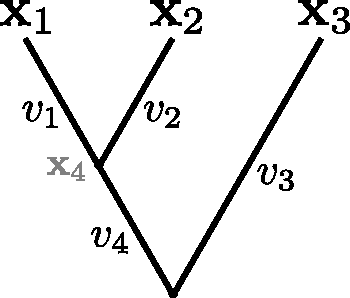
\includegraphics[scale=0.6]{pruning_example_tree_B}
	\caption[Example of phylogeny used to compute the likelihood of a multivariate Brownian-motion model using the new pruning algorithm.]{Example of phylogeny used to compute the likelihood of a multivariate Brownian-motion model using the new pruning algorithm.}
	\label{fig:example_phylo}
\end{figure}

\begin{figure}[h]
	\centering
	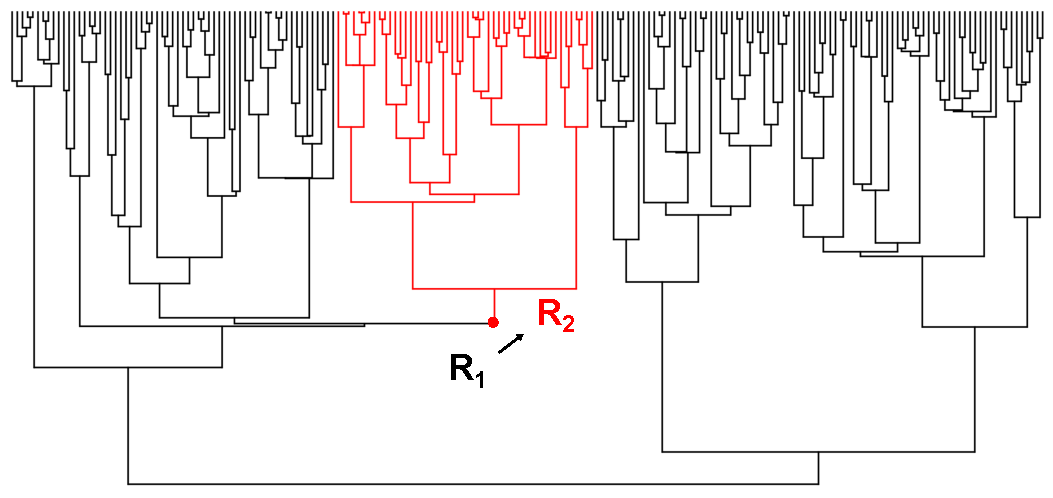
\includegraphics[scale=0.85]{phylogeny_example}
	\caption[Example of phylogeny used for the simulation study.]{Example of phylogeny used for the simulation study. We simulated phylogenies with 200 tips using a homogeneous birth-death model. Then, we randomly selected one node with exact 50 daughter tips to set the location of the transition between the background rate regime $\mathbf{R_{1}}$ and the focus clade regime $\mathbf{R_{2}}$ showed in red.}
	\label{fig:phylogeny_sims}
\end{figure}

\begin{figure}[h]
	\centering
	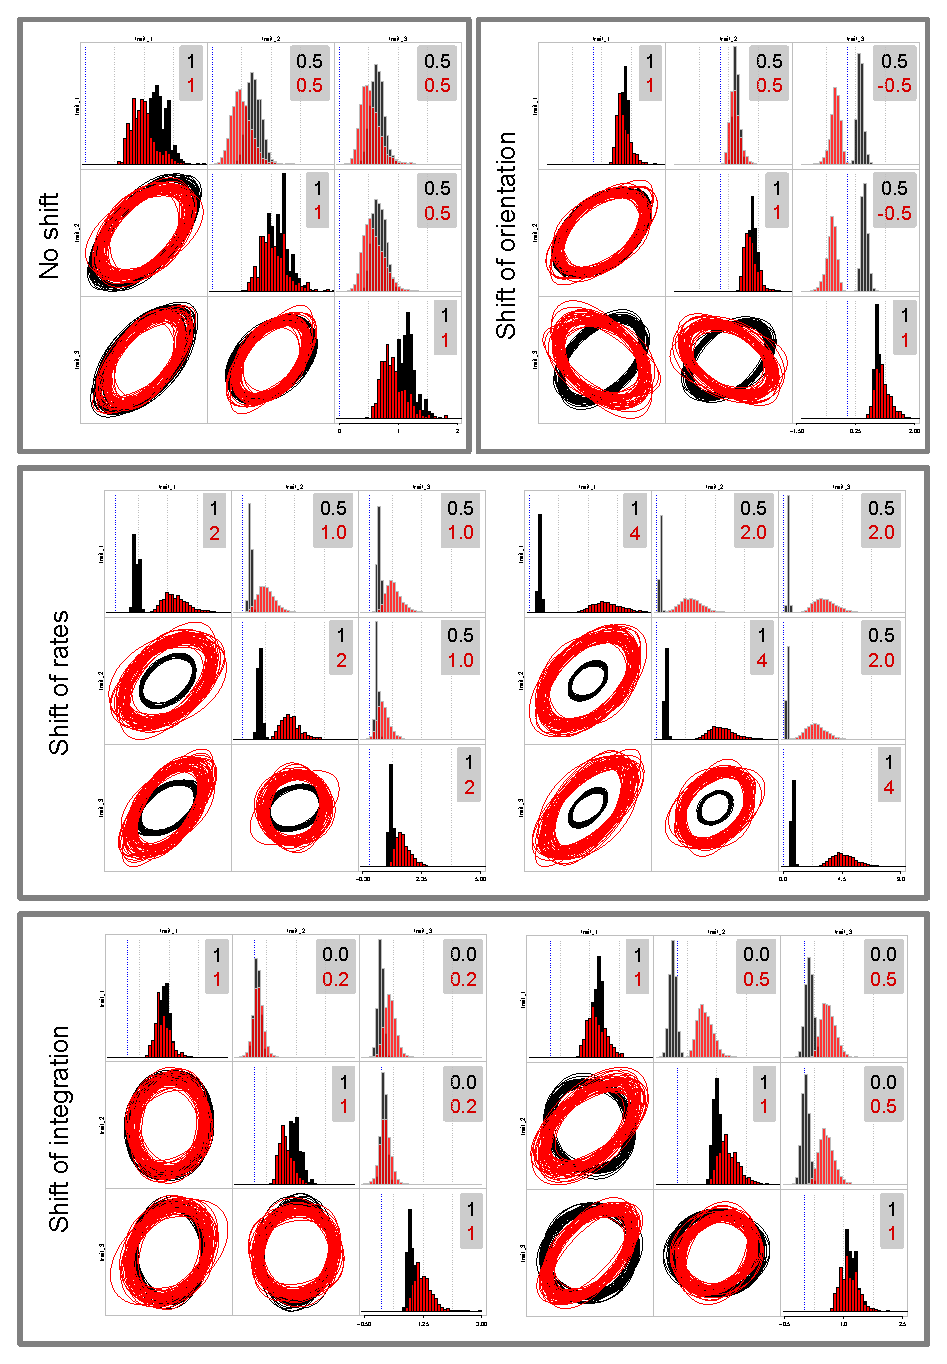
\includegraphics[scale=0.60]{posterior_sims_big_plate}
	\caption[Example of posterior distribution for the six simulation treatments with three traits each.]{Example of posterior distribution for the six simulation treatments with three traits each. Top-left plot shows the results with no shift in the evolutionary rate matrix regime and top-right shows the results with a shift in the orientation of $\mathbf{R}$. Middle row are results with a shift in the rates of evolution of each trait and bottom row shows the results when the strength of the evolutionary correlation shifts between regimes. Estimates for the background regime are showed in black and for the focus regime in red (see Fig. \ref{fig:phylogeny_sims}). For each plot: diagonal histograms show evolutionary rates (variances) for each trait, upper-diagonal histograms show pairwise evolutionary covariation (covariances), and lower-diagonal ellipses are samples from the posterior distribution showing the 95\% confidence interval of each bivariate distribution. Numbers in the top left of histograms are the true value used for each simulation; background rate regimes are showed in black and focus clade regimes in red. Table \ref{tab:model_test} shows the aggregate results for each simulation replicate: `Single' and `Orient' correspond to top-left and top-right plots. `Rates' I and II are middle row left and right plots. `Integ' I and II are bottom row left and right plots. The two replicates in the middle and bottom rows differ in the strength of the shift between regimes, left is weak and right is strong shift.}
	\label{fig:posterior_sims}
\end{figure}

\begin{figure}[h]
	\centering
	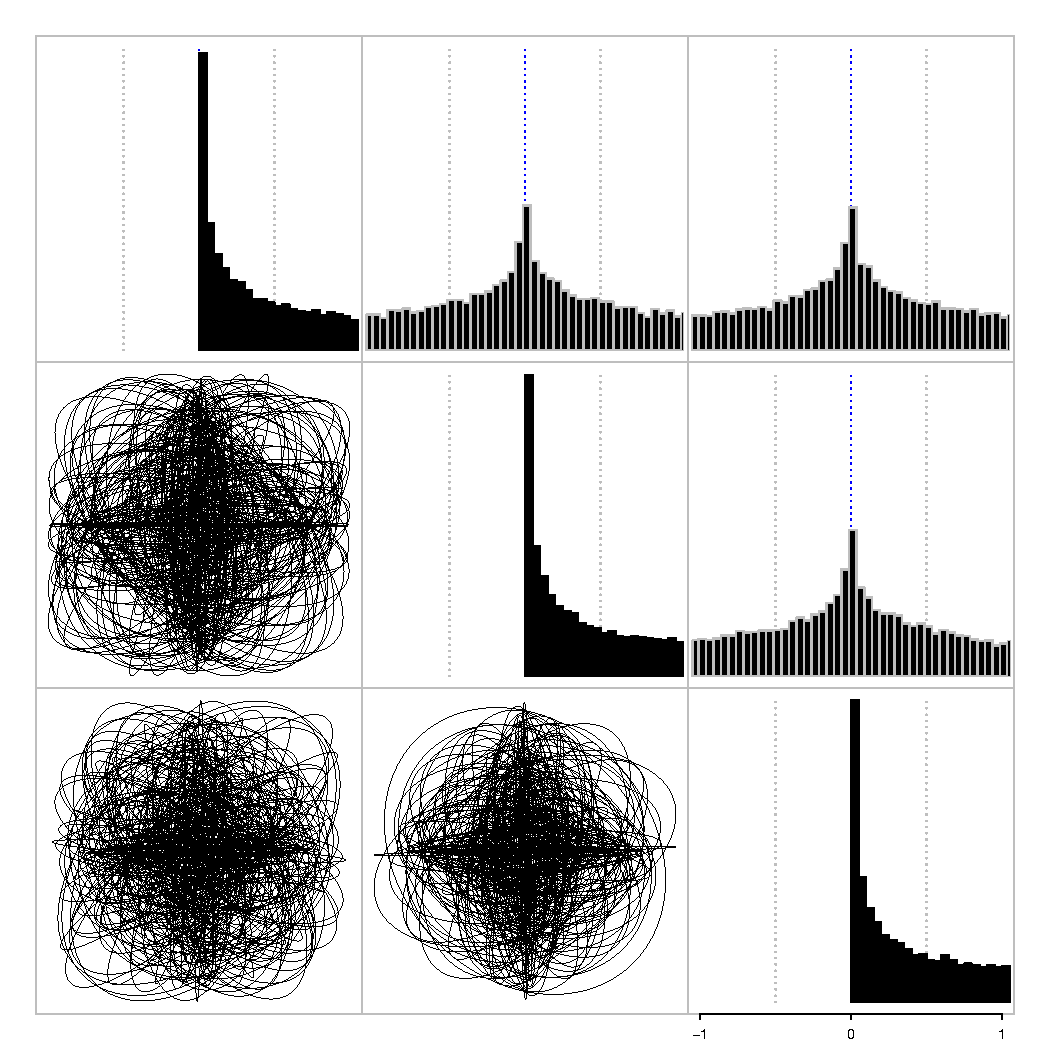
\includegraphics[scale=0.7]{prior_empirical_width_edit}
	\caption[Prior distribution for the evolutionary rate matrix ($\mathbf{R}$) used for all analyses.]{Prior distribution for the evolutionary rate matrix ($\mathbf{R}$) used for all analyses. Plate shows samples in the interval between -1 and 1 from the prior for a model with three traits. Diagonal plots represent the prior for evolutionary rates (variances) for each trait, upper-diagonal plots show pairwise evolutionary covariation (covariances), and lower-diagonal are samples from the posterior distribution of ellipses showing the 95\% confidence interval of each bivariate distribution.}
	\label{fig:prior}
\end{figure}

\begin{figure}[h]
	\centering
	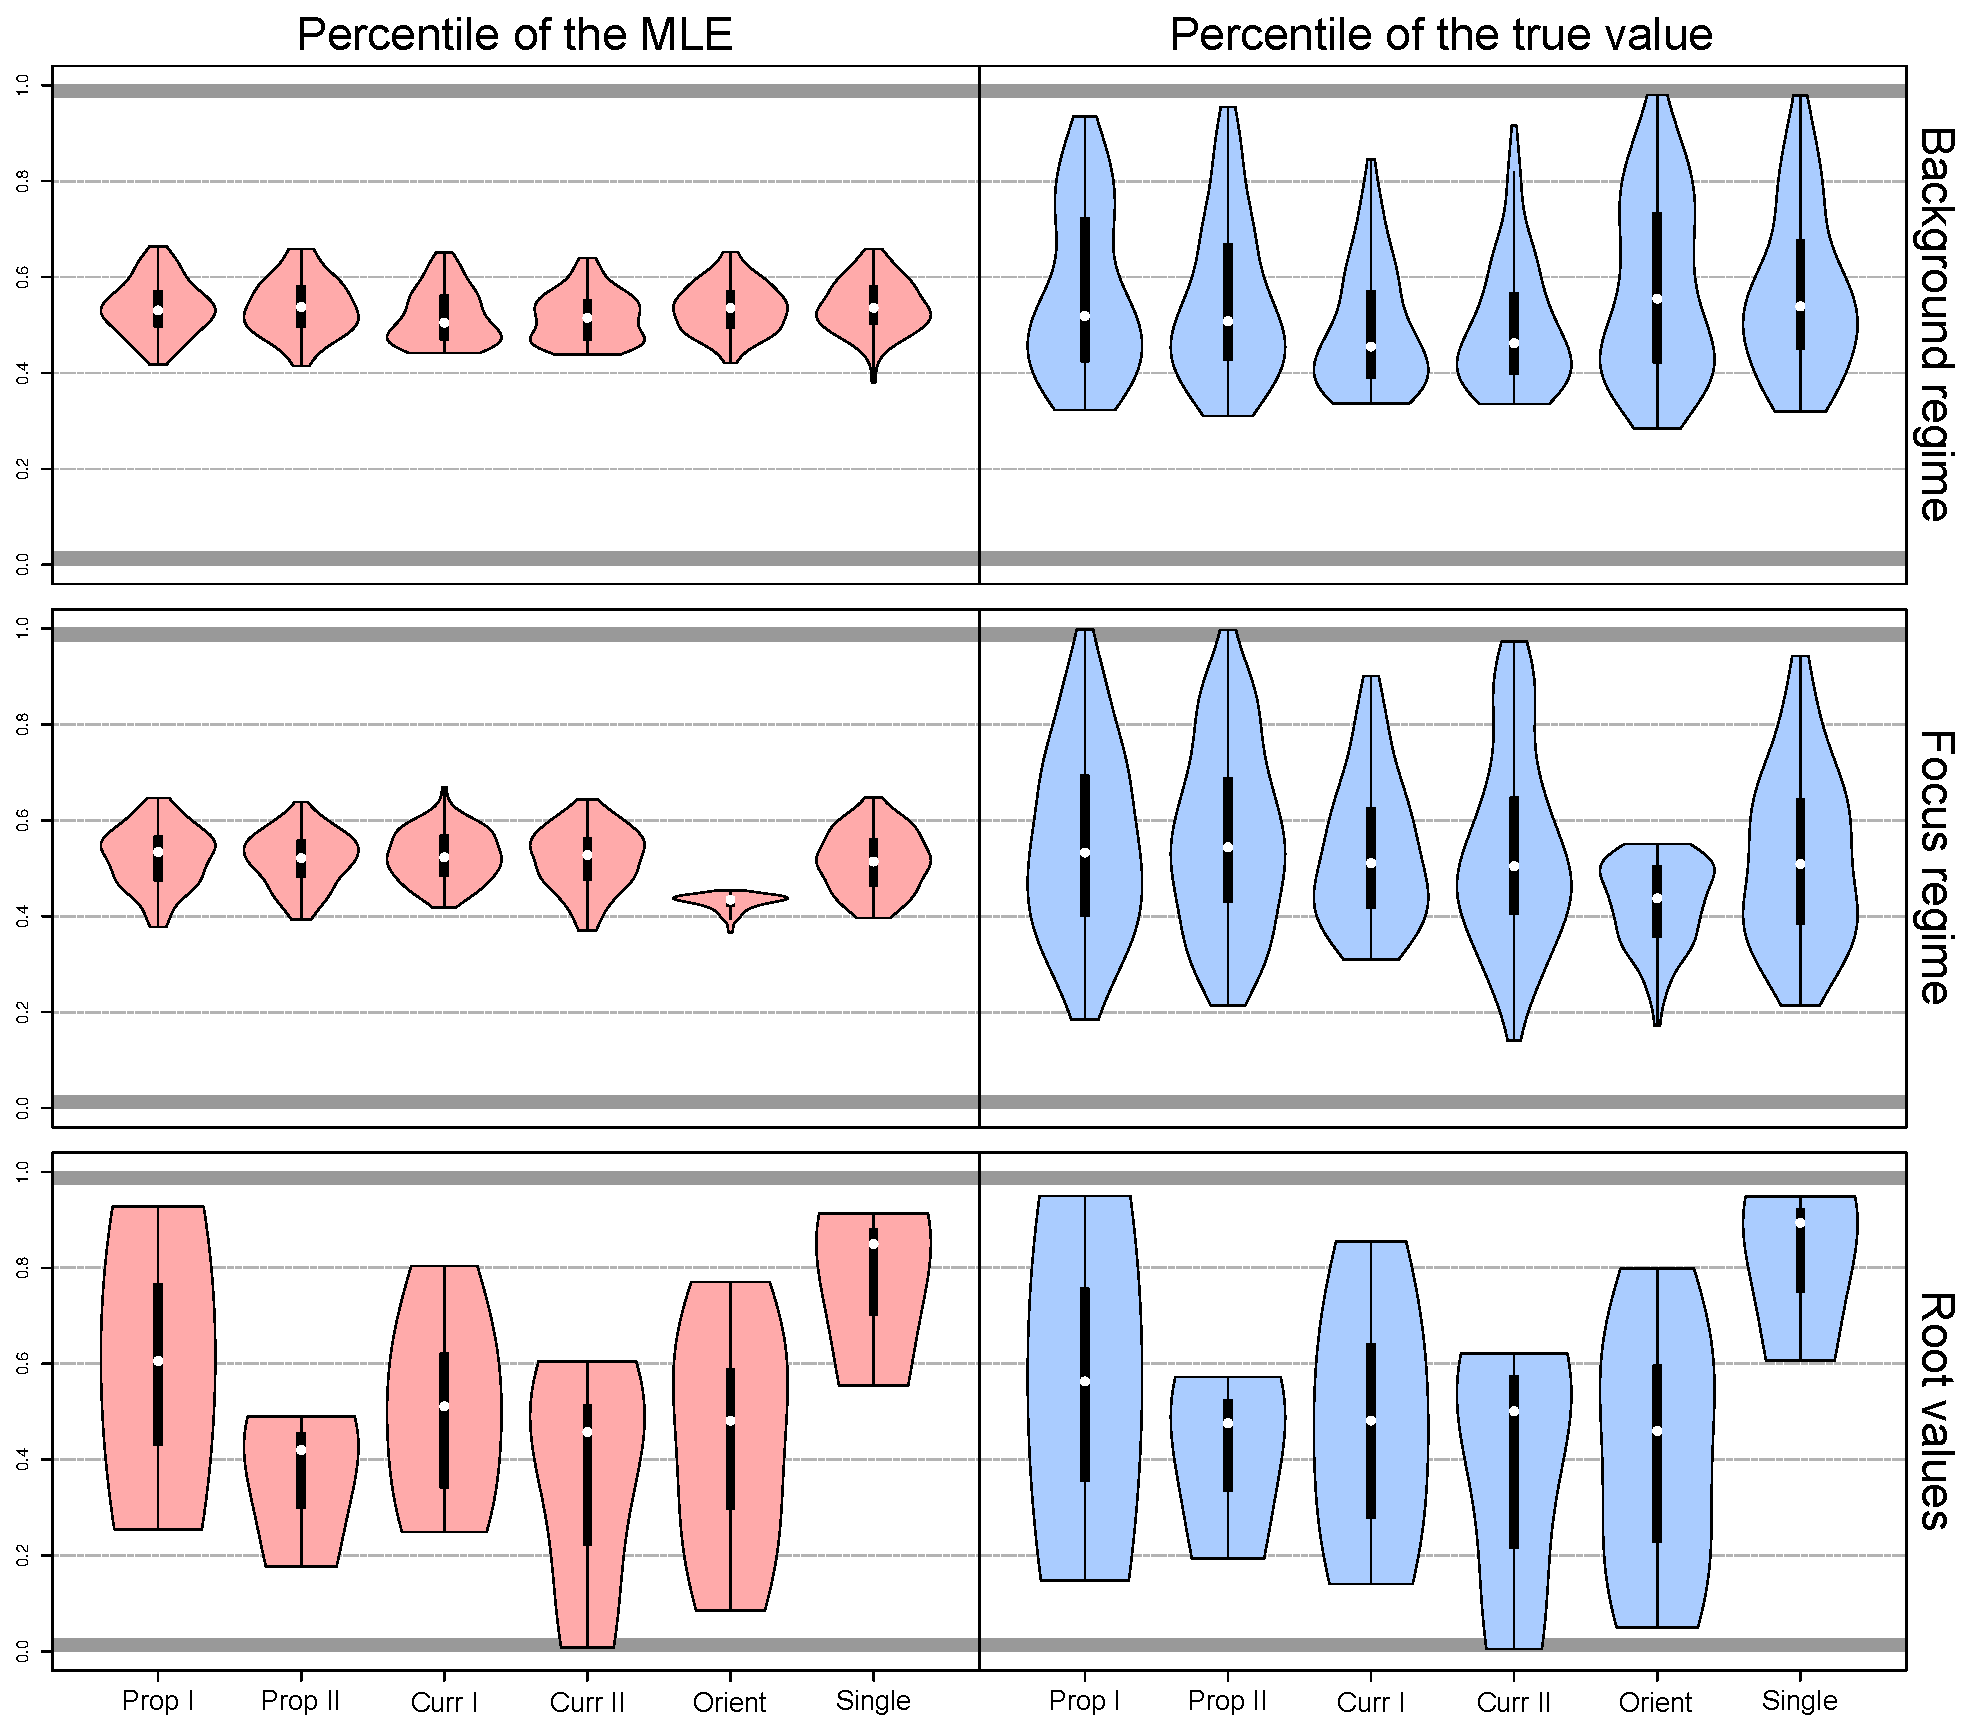
\includegraphics[scale=0.4]{percentiles_mle_true_edit}
	\caption[Distribution of percentiles for the maximum likelihood estimate (MLE) of the full model and for the true value of the simulations with respect to the posterior distribution of each simulation replicate.]{Distribution of percentiles for the maximum likelihood estimate (MLE) of the full model and for the true value of the simulations with respect to the posterior distribution of each simulation replicate. Plots to the left (pink) show the percentiles for the MLE whereas plots to the right (blue) show the percentiles for the true value of the simulations. Most of the density across all simulation scenarios and parameters is within the 95\% HPD of the posterior distribution.}
	\label{fig:quantiles}
\end{figure}

\begin{figure}[h]
	\centering
	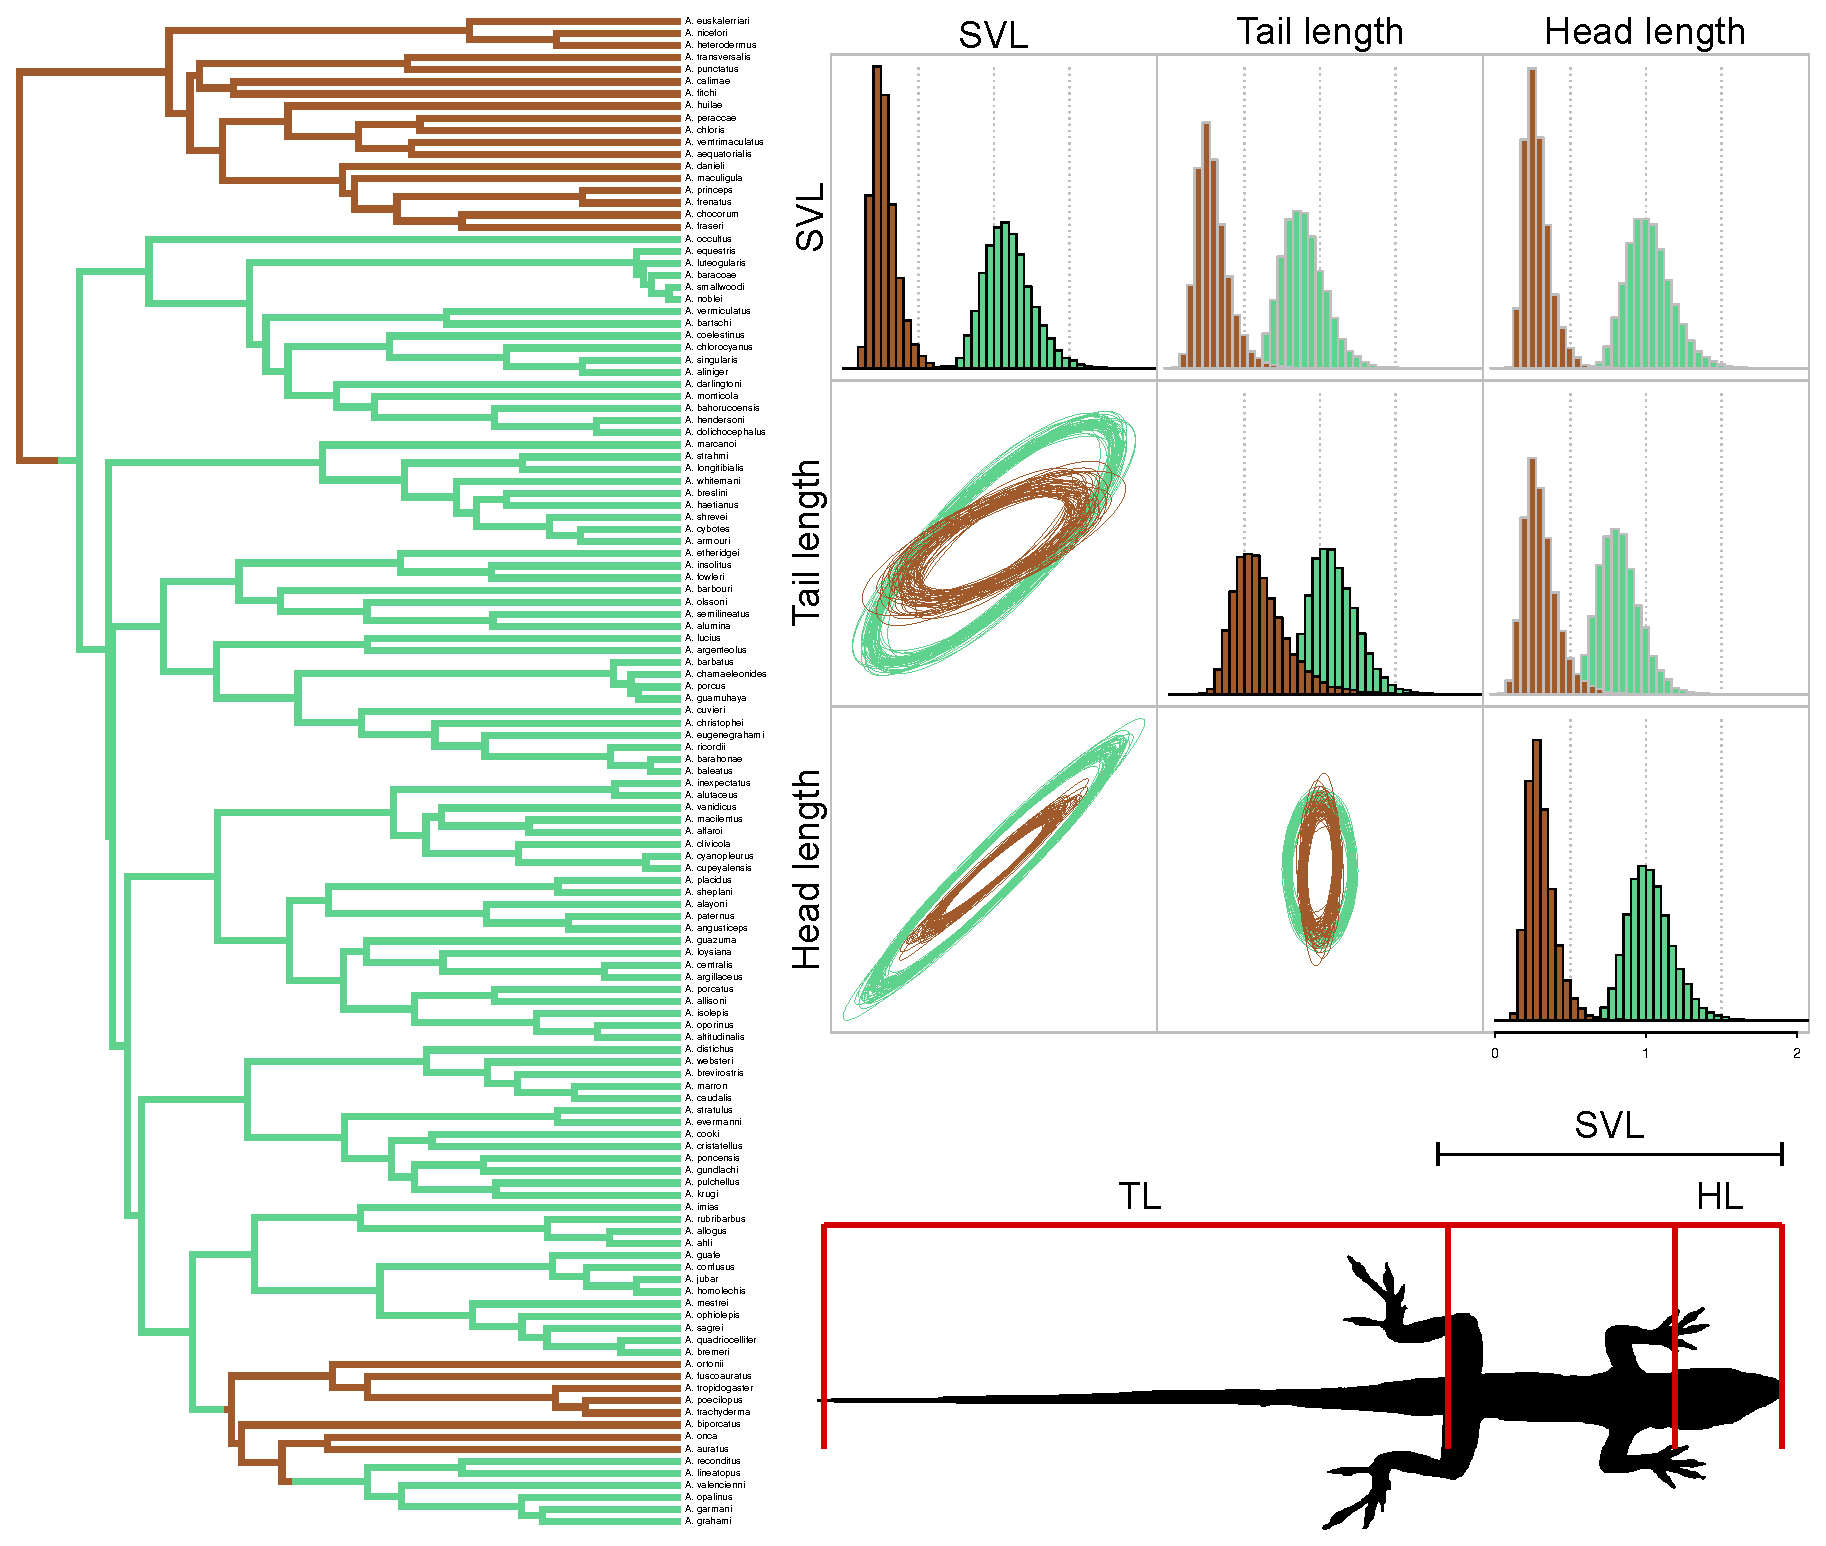
\includegraphics[scale=0.5]{anoles_figure}
	\caption[Posterior distribution of the $\mathbf{R}$ matrix regimes fitted to the island anole (green) and mainland anole (brown) lineages.]{Posterior distribution of the $\mathbf{R}$ matrix regimes fitted to the island anole (green) and mainland anole (brown) lineages. Left figure shows the maximum clade credibility tree (MCC) from \citet{gamble_anolis_2014} with only the taxa used in this study. State reconstruction for the branches was performed with a stochastic map simulation using `mainland' as the root state for the genus. Right upper plot shows the posterior distribution of parameter estimates for the evolutionary rate matrices. Diagonal plots show evolutionary rates (variances) for each trait, upper-diagonal plots show pairwise evolutionary covariation (covariances), and lower-diagonal are samples from the posterior distribution of ellipses showing the 95\% confidence interval of each bivariate distribution. Right bottom figure shows a representation of each trait (TL: tail length; HL: head length; SVL: snout-vent length).}
	\label{fig:anoles}
\end{figure}

\begin{figure}[h]
	\centering
	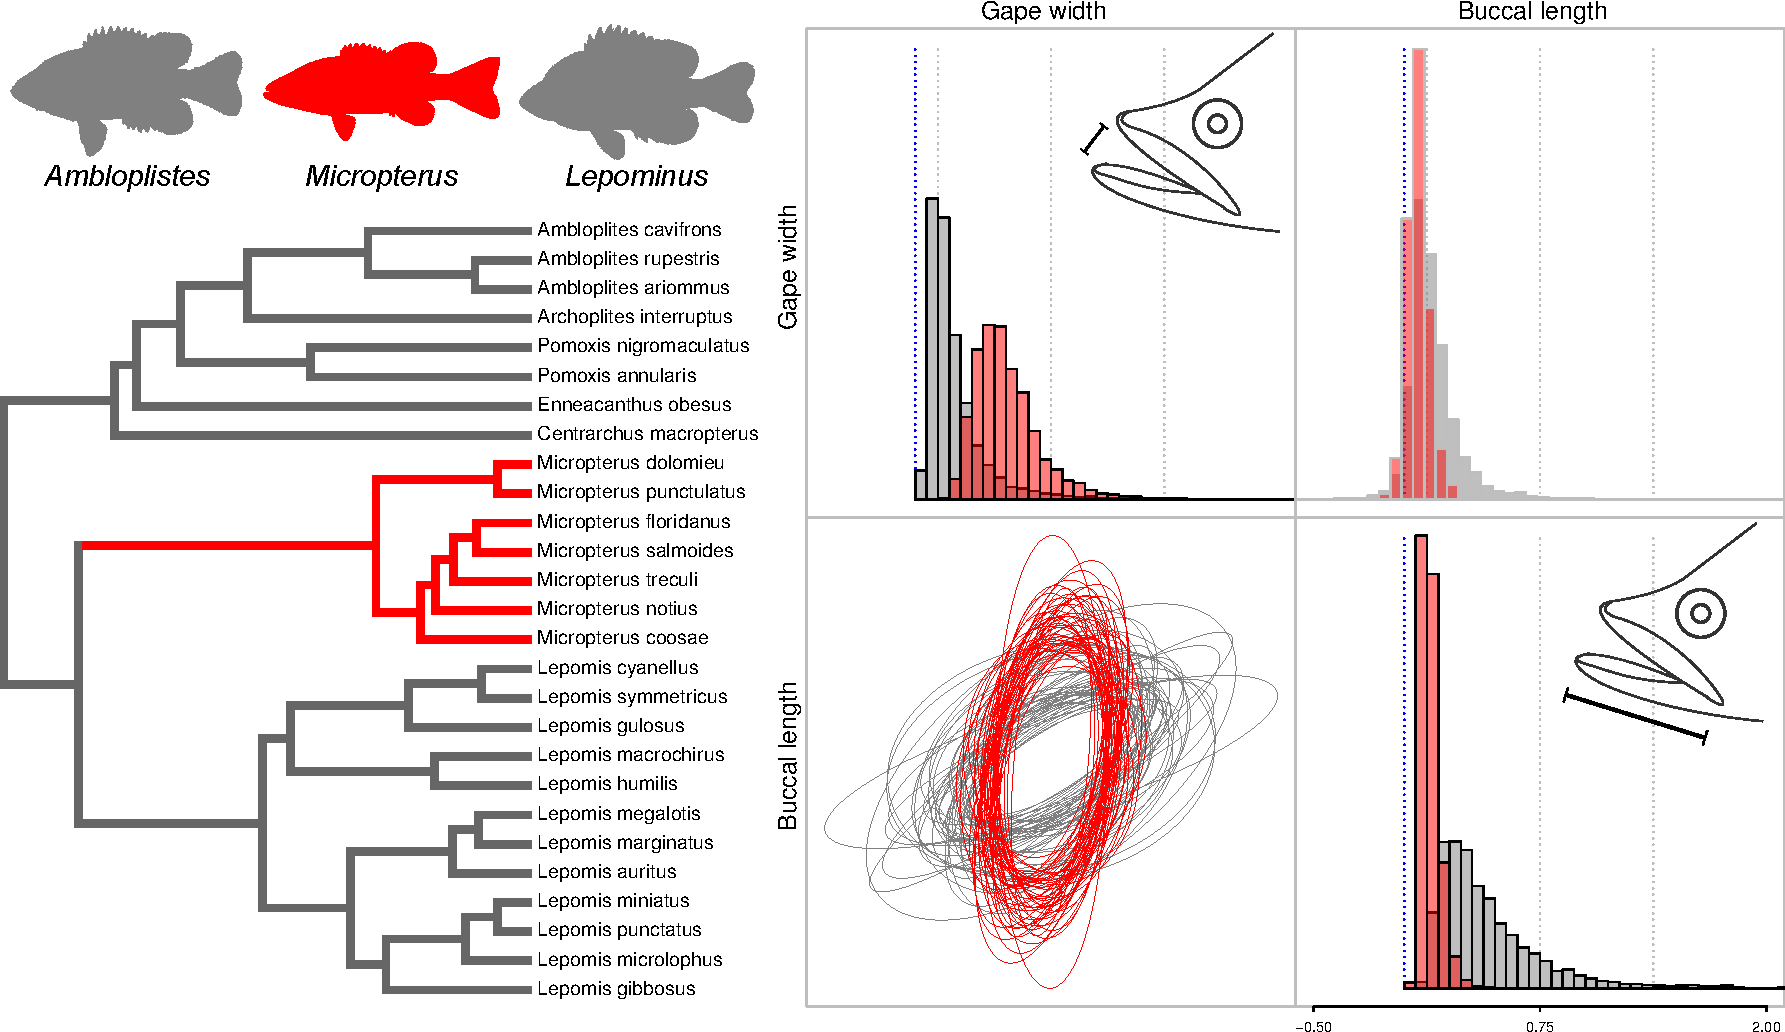
\includegraphics[scale=0.5]{results_centrarchidae}
	\caption[Posterior distribution of the $\mathbf{R}$ matrix regimes fitted to the background group and to the \textit{Micropterus} clade.]{Posterior distribution of the $\mathbf{R}$ matrix regimes fitted to the background group (gray) and to the \textit{Micropterus} clade (red). Left figure shows the phylogeny from \citep{revell_phylogenetic_2009} and the silhouette of some representatives of the Centrarchidae genera. Right plot shows the posterior distribution of parameter estimates for the evolutionary rate matrices. Diagonal plots show evolutionary rates (variances) for each trait, upper-diagonal plots show pairwise evolutionary covariation (covariances), and lower-diagonal are samples from the posterior distribution of ellipses showing the 95\% confidence interval of each bivariate distribution.}
	\label{fig:centrarchidae}
\end{figure}

\begin{figure}[h]
	\centering
	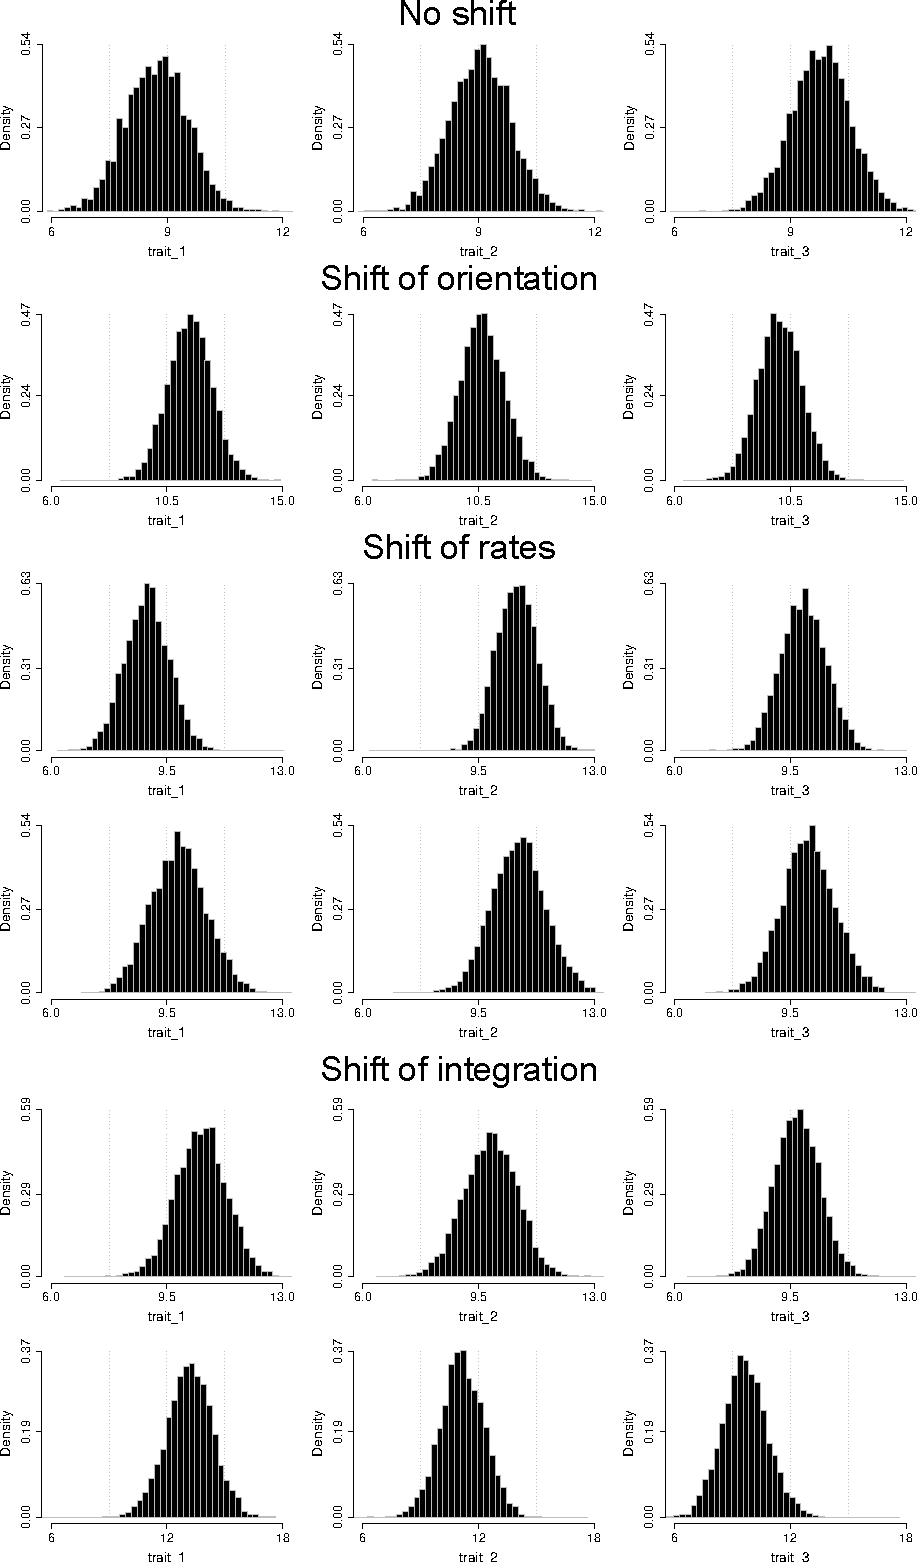
\includegraphics[scale=0.6]{root_sims_plate}
	\caption[Example of posterior distribution of root values for the six simulation treatments with three traits each.]{Example of posterior distribution of root values for the six simulation treatments with three traits each. Simulation treatments are the same as showed on Figure \ref{fig:posterior_sims}. Top and bottom plots for `Shift of rates' and `Shift of integration' treatments correspond to the left and right plots of the same treatments on Figure \ref{fig:posterior_sims}, respectively. The true value for the ancestral state of each trait in all simulations was equal to 10.}
	\label{fig:sup_root_sims}
\end{figure}

\begin{figure}[h]
	\centering
	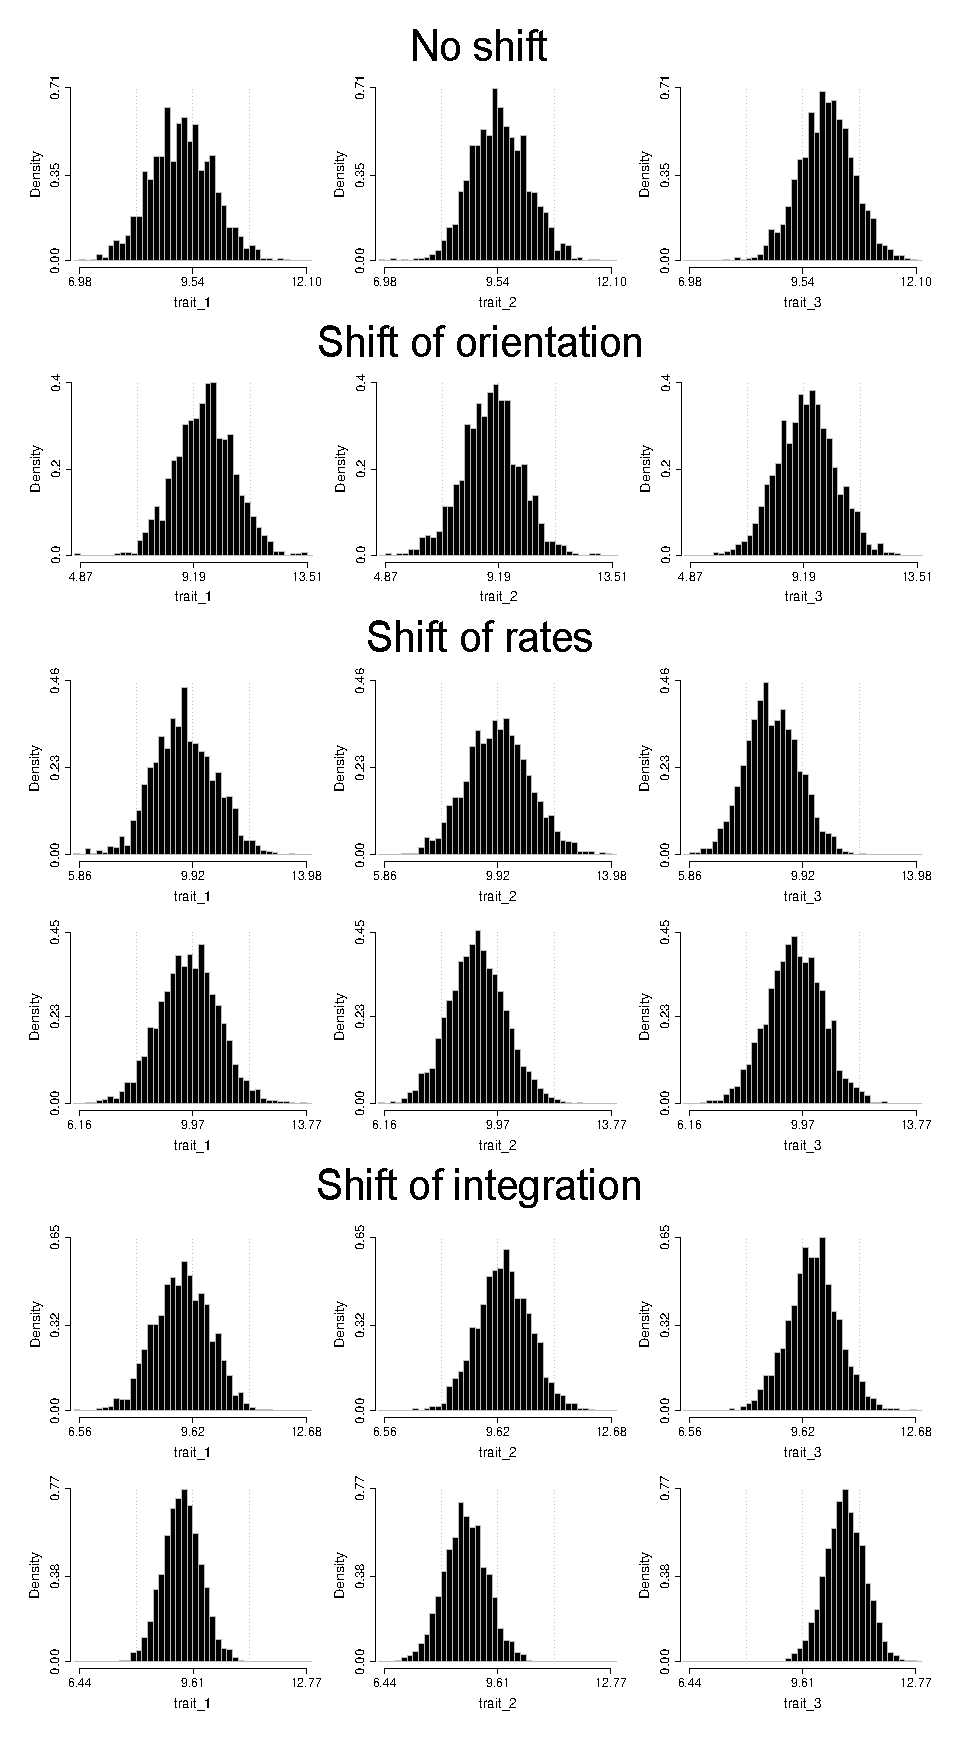
\includegraphics[scale=0.6]{plate_root_value_flat}
	\caption[Example of posterior distribution of root values for the six simulation treatments with three traits each using a uniform prior for the vector of root values.]{Example of posterior distribution of root values for the six simulation treatments with three traits each using a uniform prior for the vector of root values. Simulation treatments are the same as showed on Figure \ref{fig:posterior_sims} and Figure \ref{fig:sup_root_sims}. The true value for the ancestral state of each trait in all simulations was equal to 10.}
	\label{fig:sup_root_sims_flat}
\end{figure}

\begin{figure}[h]
	\centering
	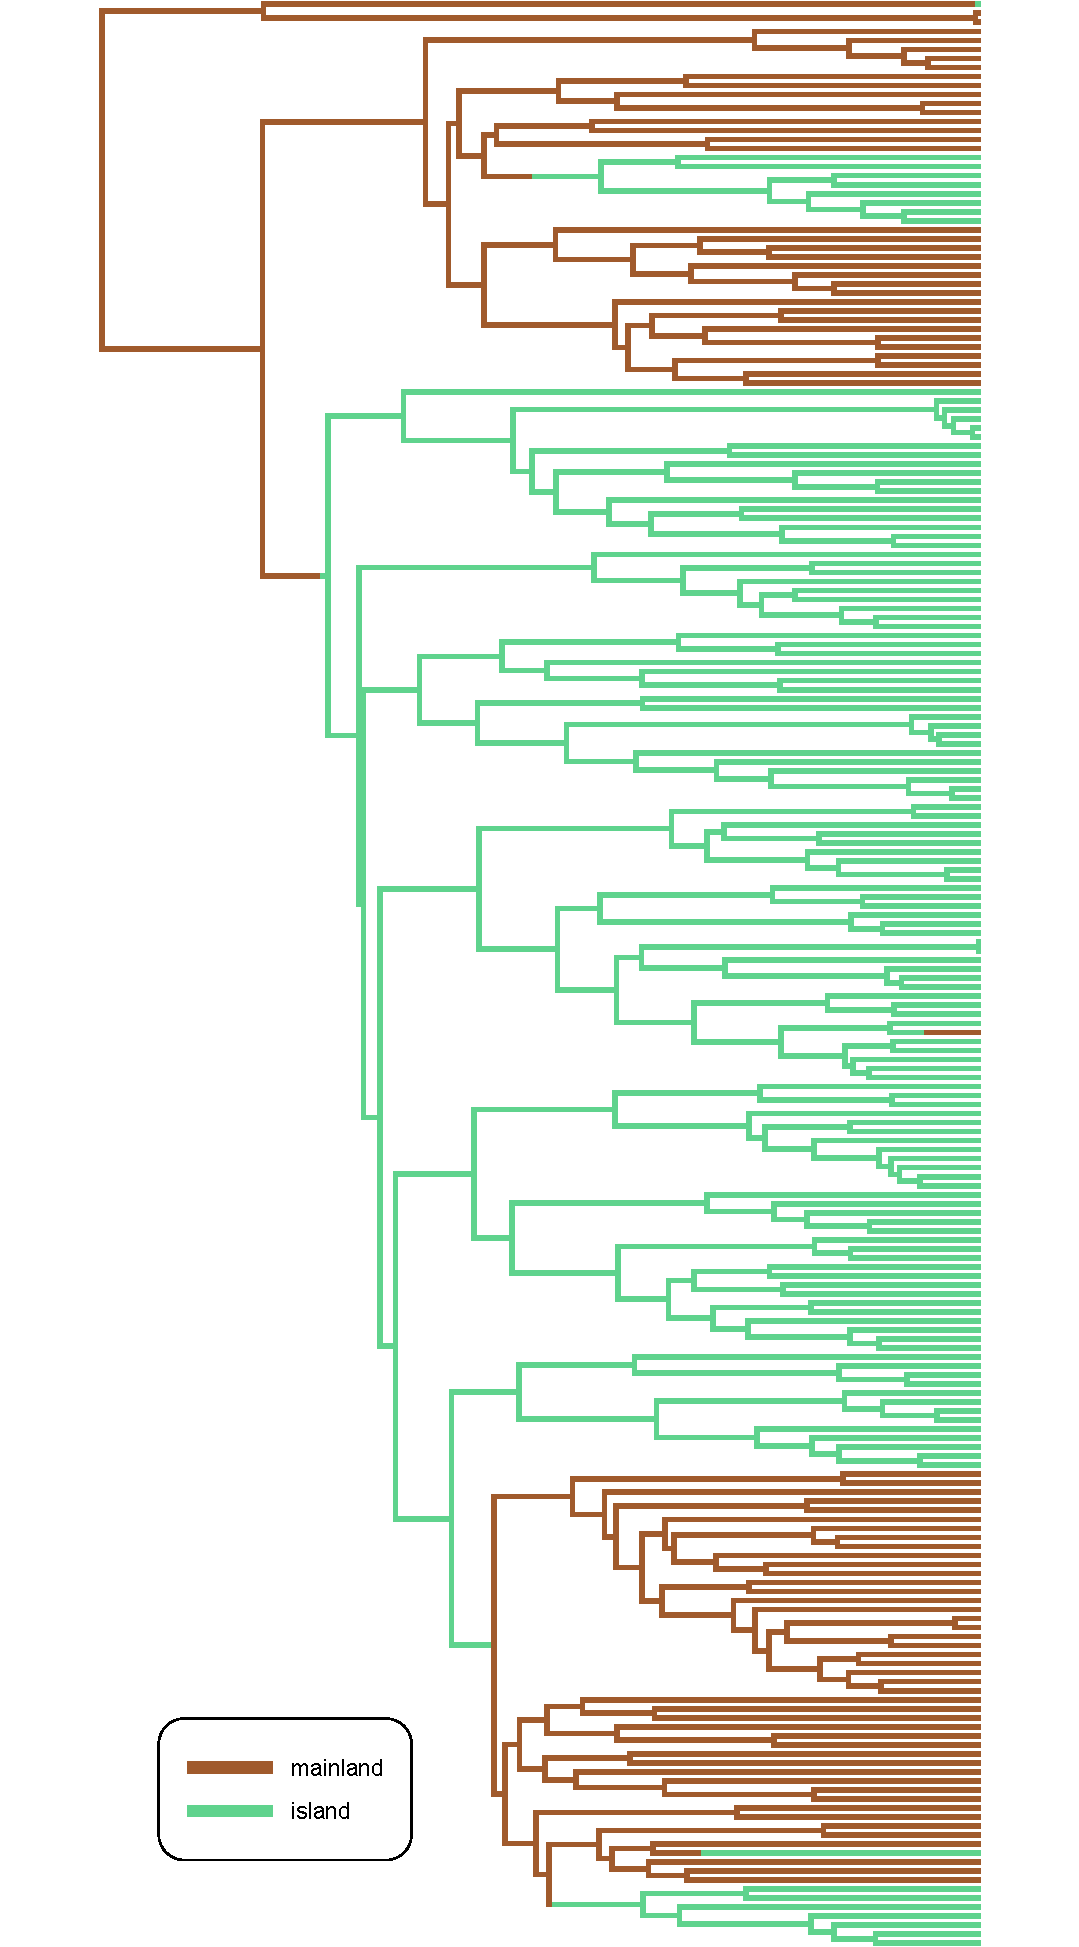
\includegraphics[scale=0.5]{Gamble_full_biogeo}
	\caption[Maximum clade credibility tree from \citet{gamble_anolis_2014} study showing the distribution of `mainland' and `island' anole species.]{Maximum clade credibility tree from \citet{gamble_anolis_2014} study showing the distribution of `mainland' and `island' anole species. The species `sp\_nov\_1', `sp\_nov\_2', and `sp\_nov\_3'  were excluded from the phylogenetic tree. Data for the distribution of anole species and outgroups were compiled from \citet{nicholson_mainland_2005}, \citet{losos_lizards_2009}, \citet{thomas_body_2009}, Reptile database (reptile-database.org) and GBIF (gbif.org). Ancestral state reconstruction was performed using stochastic mapping with the `all rates different' model and the root state set as `mainland' \citep{nicholson_mainland_2005, losos_lizards_2009}. }
	\label{fig:biogeo_gamble}
\end{figure}

\begin{figure}[h]
	\centering
	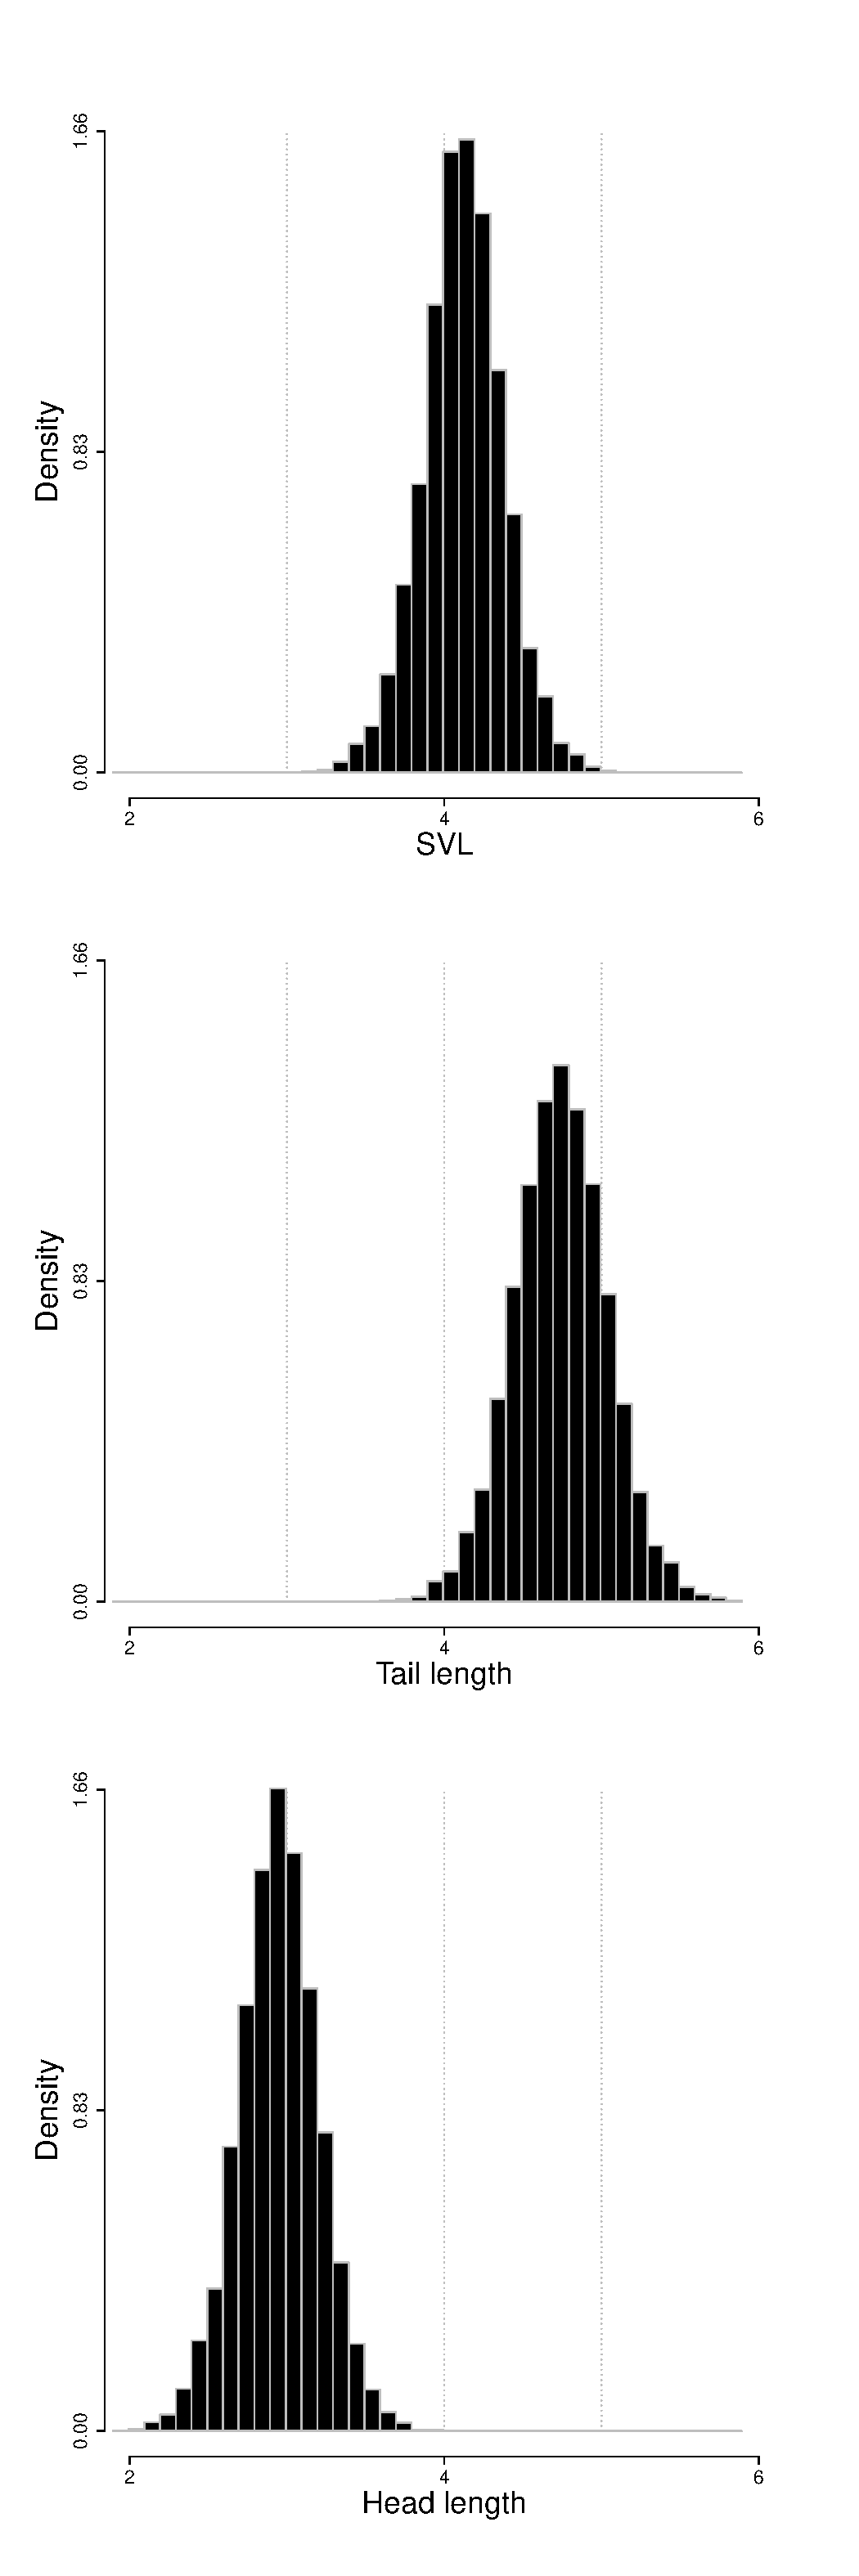
\includegraphics[scale=0.3]{anoles_root_plot}
	\caption[Posterior distribution of root values fitted to the island and mainland anole lineages.]{Posterior distribution of root values fitted to the island and mainland anole lineages (SVL: snout-vent length).}
	\label{fig:sup_root_anoles}
\end{figure}

\begin{figure}[h]
	\centering
	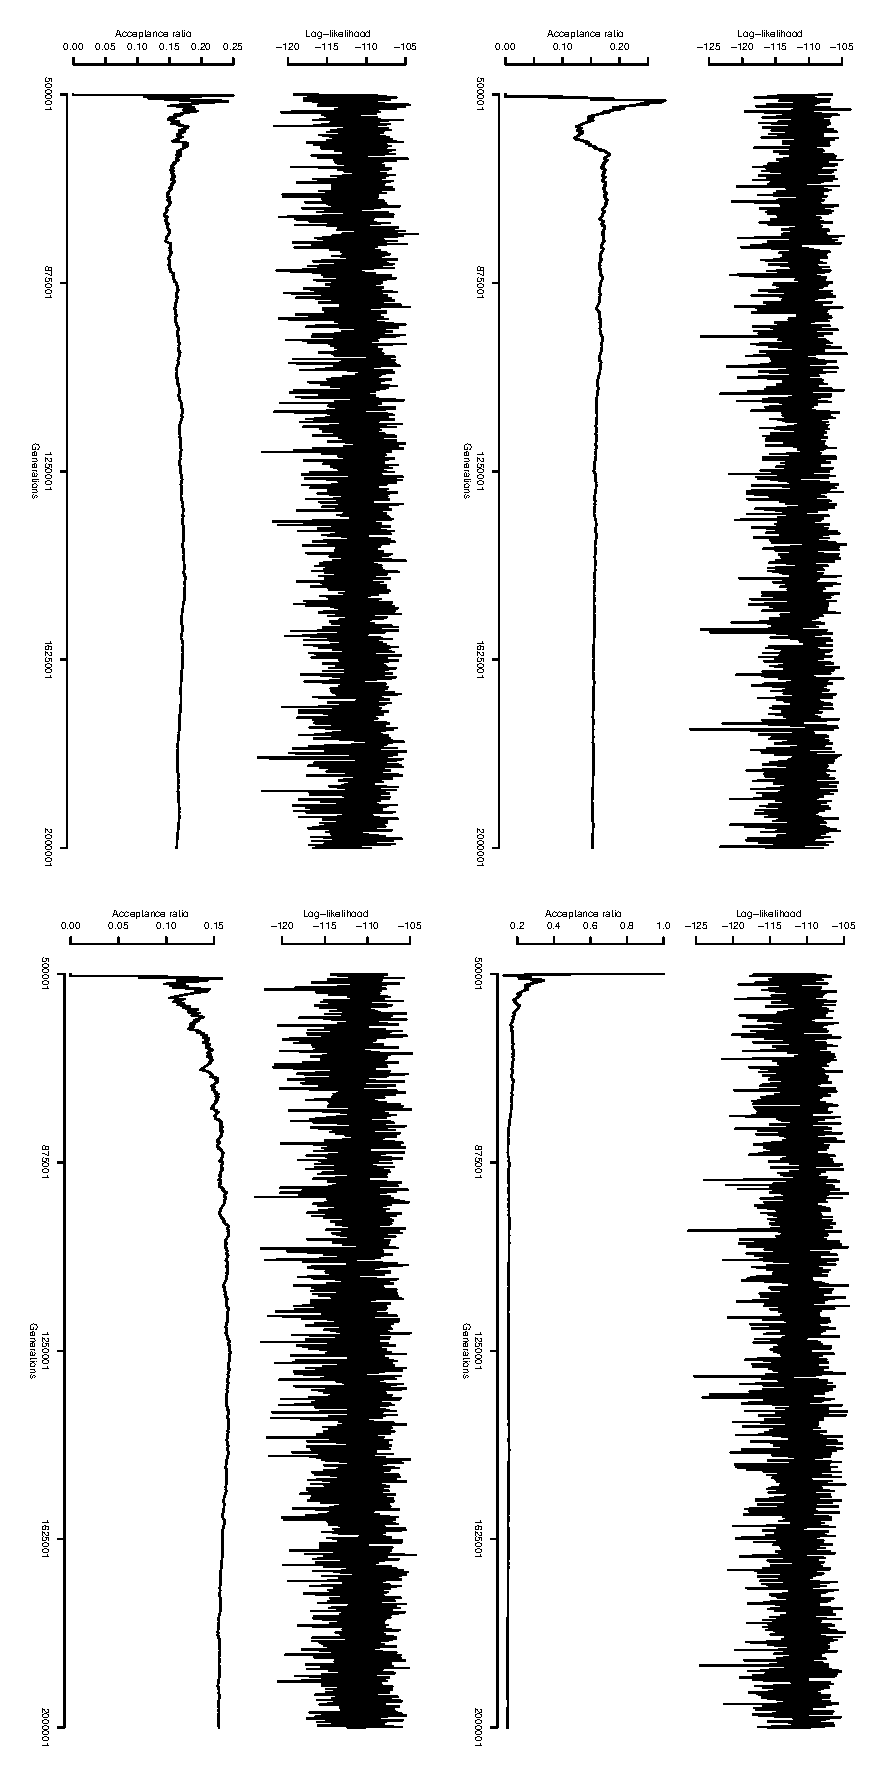
\includegraphics[scale=0.6]{anoles_log_trace_plots}
	\caption[Trace plots of the log-likelihood and the acceptance ratio for the four independent MCMC chains of the island and mainland anole analysis.]{Trace plots of the log-likelihood and the acceptance ratio for the four independent MCMC chains of the island and mainland anole analysis. }
	\label{fig:sup_trace_anoles}
\end{figure}

\begin{figure}[h]
	\centering
	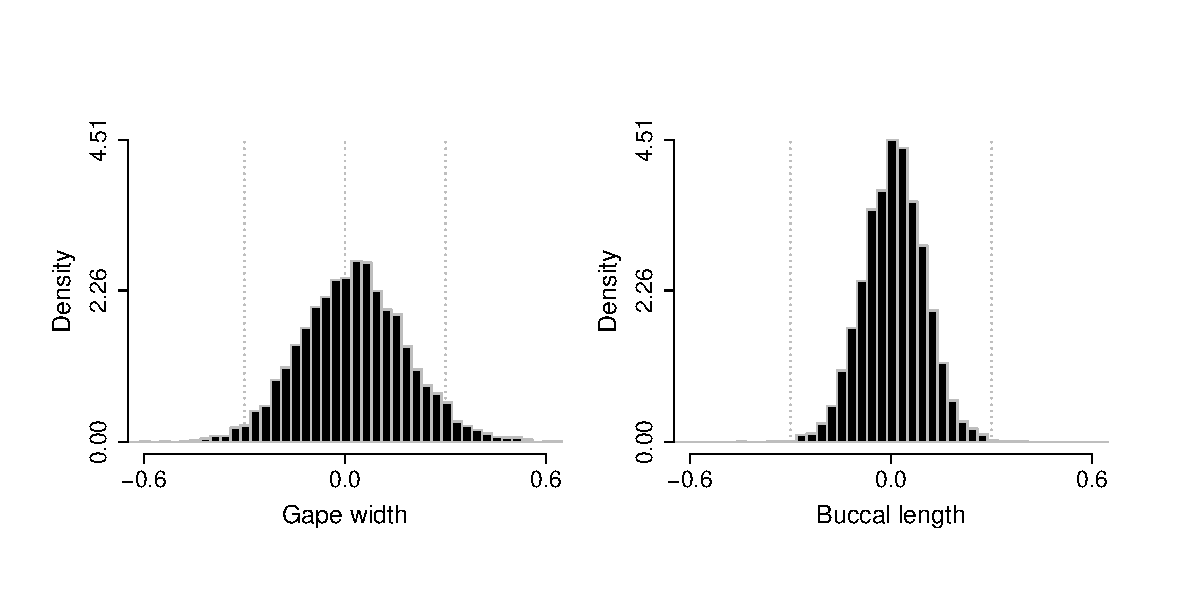
\includegraphics[scale=0.7]{root_plot_centrarchidae}
	\caption[Posterior distribution of root values fitted to the Centrarchidae fishes.]{Posterior distribution of root values fitted to the Centrarchidae fishes.}
	\label{fig:sup_root_centrarchidae}
\end{figure}

\begin{figure}[h]
	\centering
	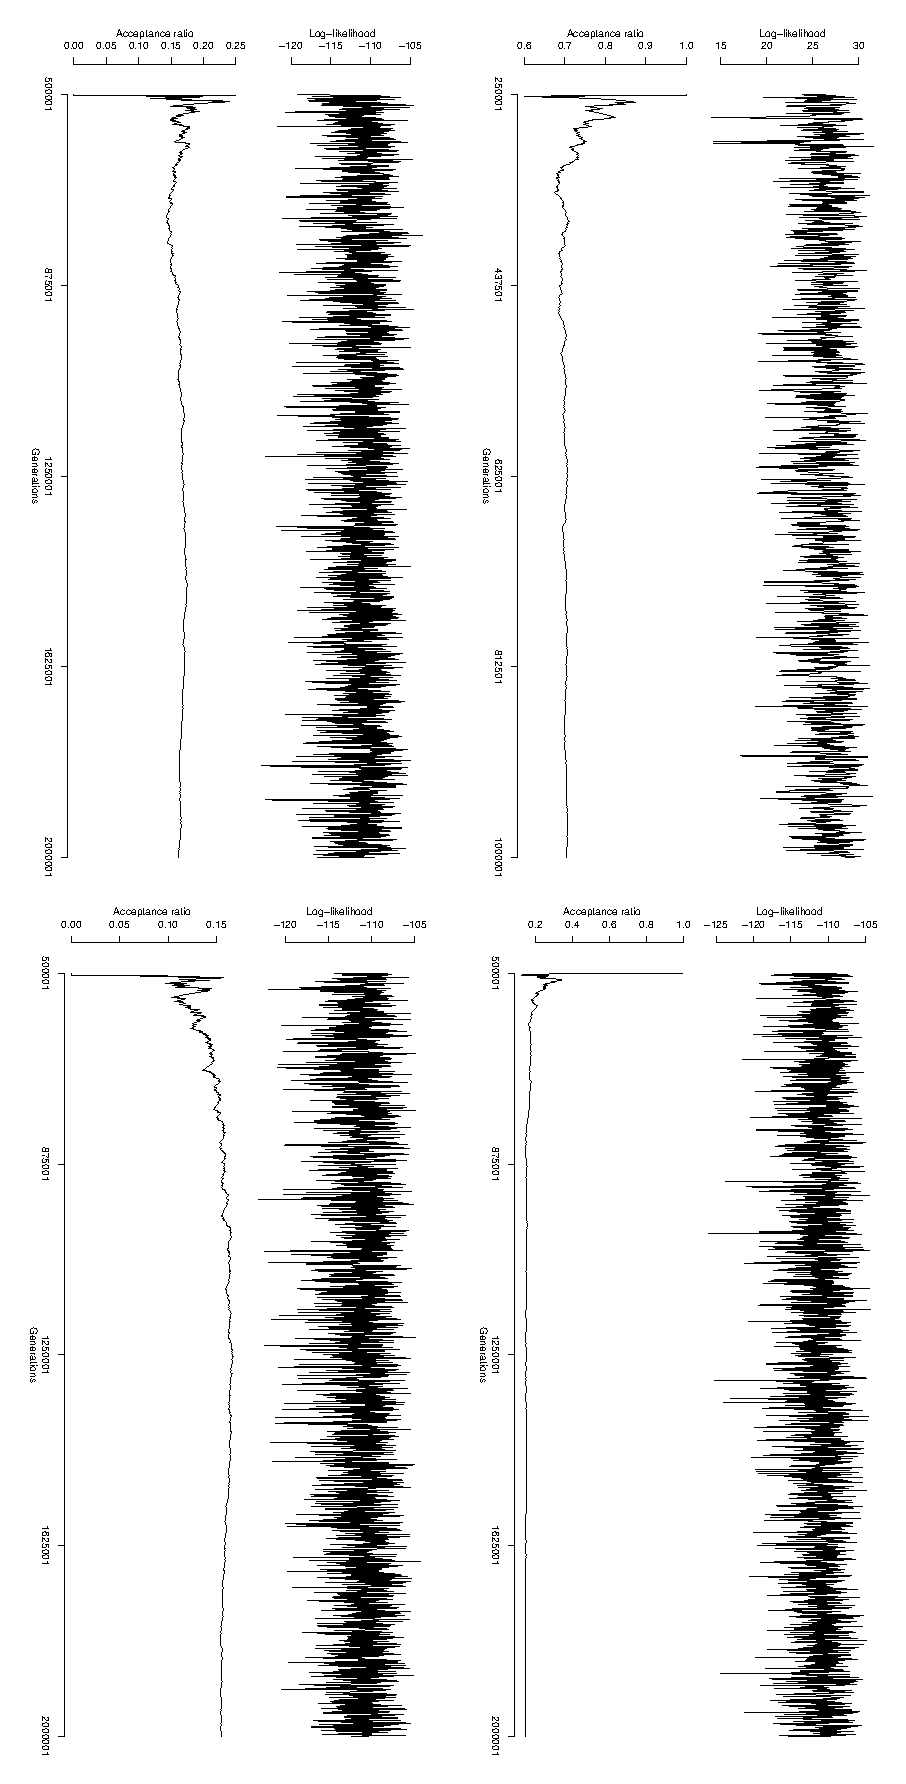
\includegraphics[scale=0.6]{trace_plots_centrarchidae}
	\caption[Trace plots of the log-likelihood and the acceptance ratio for the four independent MCMC chains of the Centrarchidae fishes analysis.]{Trace plots of the log-likelihood and the acceptance ratio for the four independent MCMC chains of the Centrarchidae fishes analysis. }
	\label{fig:sup_trace_centrarchidae}
\end{figure}

\begin{figure}[h]
	\centering
	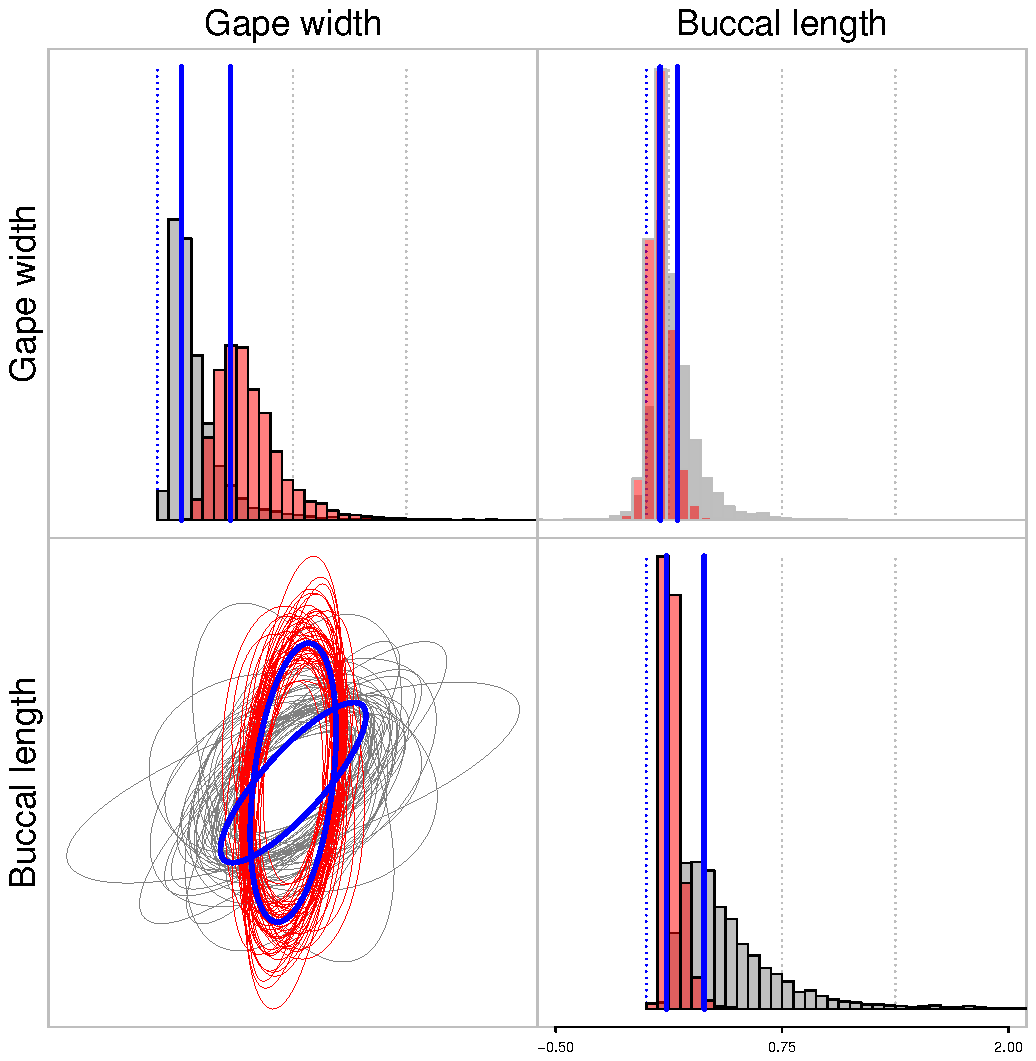
\includegraphics[scale=0.6]{centrarchidae_compare_with_mle}
	\caption[Posterior distribution of the $\mathbf{R}$ matrix regimes fitted to the background group and to the \textit{Micropterus} clade.]{Posterior distribution of the $\mathbf{R}$ matrix regimes fitted to the background group (gray) and to the \textit{Micropterus} clade (red). Maximum likelihood estimate for the same data and phylogenetic tree showed in blue lines. Plot shows the posterior distribution of parameter estimates for the evolutionary rate matrices. Diagonal plots show evolutionary rates (variances) for each trait, upper-diagonal plot show pairwise evolutionary covariation (covariances), and lower-diagonal plot shows samples from the posterior distribution of ellipses showing the 95\% confidence interval of each bivariate distribution.}
	\label{fig:centrarchidae_mle}
\end{figure}

% \addtocontents{toc}{\protect\newpage} % To make table of contents start in the next page.
%% This is the Chapter 3

%\begin{hyphenrules}{nohyphenation}
\chapter{AN R PACKAGE FOR STUDYING EVOLUTIONARY INTEGRATION AMONG SEVERAL TRAITS ON PHYLOGENETIC TREES}
%\end{hyphenrules}

\section{Abstract}

Evolutionary integration occurs when two or more phenotypes evolve in a correlated fashion. Correlated evolution among traits can happen due to genetic constraints, ontogeny, and selection and have an important impact on the trajectory of phenotypic evolution. Phylogenetic trees can be used to study such pattern on macroevolutionary time scales by estimating the strength of evolutionary covariance among traits through time and across clades. However, only few applications implement models to conduct comparative analyses of evolutionary integration. We introduce a Bayesian Markov chain Monte Carlo approach to estimate the evolutionary correlation among two or more traits using the evolutionary rate matrix ($\mathbf{R}$). $\mathbf{R}$ is a covariance matrix that represents both the rates of evolution of each trait and the structure of evolutionary correlation among traits. Here we present the R package \texttt{ratematrix}, a resource to test hypotheses of evolutionary integration using multivariate data and phylogenetic trees. \texttt{ratematrix} provides a flexible framework allowing for any number of evolutionary rate matrix regimes fitted to the same phylogenetic tree and it incorporates the uncertainty associated with parameter estimates, ancestral state reconstruction and phylogenetic estimation in the analyses. The \texttt{ratematrix} package uses a novel pruning algorithm that significantly improve computational time. We also provide specific functions that facilitate users to conduct long MCMC analysis when computational resources are limited.

\section{Introduction}

Evolutionary changes in one trait are often associated with changes in other traits, such that species traits often do not vary independently of each other \citep{Olson_Miller_1958}. This pattern can be observed in the covariation among traits both within and among populations \citep{arnold_constraints_1992, arnold_adaptive_2001, revell_testing_2008, revell_phylogenetic_2009}. The pattern of correlated evolutionary changes among two or more traits is known as evolutionary integration and can be a result of genetic constraints (e.g., pleiotropy), ontogenetic integration, or correlated selection \citep{arnold_constraints_1992, arnold_adaptive_2001, pigliucci_evolvability_2004, goswami_fossil_2015, melo_modularity:_2016}. Although evolutionary integration is ubiquitous across the tree of life, only few comparative methods and associated software applications to date implement models that can estimate evolutionary correlations among traits using phylogenetic trees \citep{revell_testing_2008, hohenlohe_mipod:_2008, revell_phylogenetic_2009, bartoszek_phylogenetic_2012, adams_geomorph:_2013, Clavel_mvmorph, goolsby_rphylopars:_2016}. 

Here we describe the R package \texttt{ratematrix}, which implements a Bayesian estimate of evolutionary rate matrices \citep[ $\mathbf{R}$;][]{revell_testing_2008} fitted to phylogenetic trees and trait data using Markov chain Monte Carlo \citep[as described in][]{caetano_sysbio_2017}. The $\mathbf{R}$ matrix is a variance-covariance matrix that describes the rates of trait evolution under Brownian motion in the diagonals and the evolutionary covariance among traits (i.e., the pattern of evolutionary integration) in the off-diagonals \citep{revell_testing_2008, revell_phylogenetic_2009, adams_assessing_2014}. With such a matrix we are able to simultaneously investigate the pace of evolution and the structure of evolutionary integration among two or more continuous traits evolving along the branches of a phylogenetic tree. We can also fit multiple $\mathbf{R}$ matrices to the same tree in order to test hypothesis of shifts in the evolutionary integration of these traits across clades on the tree. 

The $\mathbf{R}$ matrix can be estimated using current R packages, however all available implementations rely on point estimates using maximum likelihood. In contrast, the use of a Bayesian framework, as presented here, allows for direct incorporation of uncertainty in parameter estimates in the form of a posterior distribution \citep{caetano_sysbio_2017}. This is especially important because covariances can be hard to estimate when the number of observations is small relative to the number of parameters in the model, which is commonplace among phylogenetic comparative studies in general.

\section{ The model and MCMC implementation }

To study the pattern of correlated evolution among two or more continuous traits we use the model described by \citet{revell_testing_2008}, which consists of a multivariate Brownian motion model with rate equal to the $\mathbf{R}$ matrix and root value equal to the vector $\mathbf{a}$ \citep[see Equations 2 and 3 in][]{revell_phylogenetic_2009}. Our implementation allows for multiple independent rate regimes fitted to different branches of the phylogenetic tree \citep[as in][]{revell_phylogenetic_2009}. Rate regimes can be either fixed \textit{a priori} or a collection of multiple regime configurations can be included in the analysis. For example, multiple regimes applied to the same analysis could be samples from a stochastic character mapping \citep{huelsenbeck_stochastic_2003}, alternative reconstructions due to missing data, or other plausible hypotheses. However, all regimes need to share the same data at the tips of the tree and same number of rate matrices fitted to the tree. The \texttt{ratematrix} package implements Metropolis-Hastings Markov chain Monte Carlo (MCMC) to estimate the posterior distribution of each $\mathbf{R}$ matrix fitted to the tree and the vector of phylogenetic root values ($\mathbf{a}$).

Here we detail the proposal distribution used for each set of parameters as well as the options of prior densities currently implemented in the package. At each step of the MCMC chain we choose between the vector of root values and the set of one or more $\mathbf{R}$ matrices by drawing from a binomial distribution. The probability that each of these two sets of parameters will be updated is fixed throughout the chain, but can be determined by the user (see function \texttt{ratematrixMCMC}). Every time that the set of rate matrices is chosen, only one $\mathbf{R}$ matrix is updated but all $\mathbf{R}$ matrices fitted to the tree are equally likely to be updated. In contrast, once chosen, the root value for every trait is updated simultaneously. Updates are performed with different configurations of sliding window proposal distributions.

We implemented a uniform distribution with width controlled by the parameter \texttt{`w\_mu'} as the proposal distribution for each element of the vector of phylogenetic means. In contrast, the proposal of $\mathbf{R}$ matrices requires a more elaborate scheme, since variance-covariance matrices are constrained to be positive definite. Furthermore, $\mathbf{R}$ matrices describe both the rate of evolution of the traits and their pattern of evolutionary correlation, so the proposal distribution needs to provide good mixing for both the variance of each trait and the correlation structure of such matrices. We implemented a separation strategy \citep{barnard_modeling_2000, zhang_sampling_2006, liu_comparison_2016} proposal scheme which consists of making updates to the vector of standard deviations and the correlation matrix derived from the variance-covariance matrix in separate steps (Figure \ref{fig:proposal}). The vector of standard deviations can be updated directly using a sliding window proposal distribution. On the other hand, the proposal scheme for the correlation matrix requires two steps: first, draw covariance matrices from an inverse-Wishart distribution; and second, we derive correlation matrices from this sample. Finally, we recompose the evolutionary rate matrix in order to calculate the likelihood of the model. Figure \ref{fig:proposal} shows a diagram that describes the procedure. Note that the vector of standard deviations generated by decomposing the variance-covariance matrix is not evaluated by the likelihood of the model \citep{zhang_sampling_2006}. As a result of this parameter-extension approach, we need to correct the acceptance ratio for the transformation from variance-covariance matrix to the corresponding correlation matrix and vector of variances (Figure \ref{fig:proposal}). This proposal scheme allows for independent priors and proposals for the rates of evolution and the evolutionary integration among traits. The \texttt{ratematrix} package allows control over the width of the uniform sliding window proposal for the vector of standard deviations (`\texttt{w\_sd}') as well as the degrees of freedom of the inverse-Wishart (`\texttt{v}') used to sample correlation matrices.

\pagebreak

The prior densities for the model naturally follow the proposal scheme implemented. Prior densities are determined for the vector of root values, the vector of standard deviations and the correlation matrix (which is sampled by a transformation from the inverse-Wishart distribution). The separation between standard deviations and correlation matrix enable users to translate their biological intuition about the pace and mode of evolution into model parameters in a straightforward manner. The user can set independent priors (options are uniform, normal or log-normal) for both the vector of root values and the vector of standard deviations of the $\mathbf{R}$ matrices. For the correlation matrix that, together with the standard deviation, will constitute the $\mathbf{R}$ matrix the user can set the degrees of freedom ($\nu$) and the scale matrix ($\Psi$) of the inverse-Wishart distribution. Small values for $\nu$ make the distribution wider (Figure \ref{fig:prior_samples}, top) whereas larger values reduce the variance of the distribution, so samples will be closer to $\Psi$ and, as a result, the prior will be more informative (Figure \ref{fig:prior_samples}, bottom). Note from Figure \ref{fig:prior_samples} that a change in the parameters of the inverse-Wishart prior on the correlation matrix will not change the prior distribution of variances. Since the inverse-Wishart will only be used to sample correlation matrices, $\Psi$ can be set as any correlation matrix or variance-covariance matrix.

\section{ Description of the \texttt{ratematrix} R package }

The package \texttt{ratematrix} offers a plethora of functions to allow flexible choices of prior distributions for all parameters in the model, customizable MCMC chains, plots, and robust analyses of convergence (Table \ref{tab:functions}). The package can be installed from our \texttt{github} repository using the R package \texttt{devtools}:\\
\\
\hspace*{20pt} \texttt{ devtools::install\_github("Caetanods/ratematrix", build\_vignettes = TRUE) }
\hspace*{20pt} \texttt{ library(ratematrix) }\\
\\
The option \texttt{build\_vignettes} will make the package vignettes available after installation. A list of vignettes can be accessed using:\\
\\
\hspace*{20pt} \texttt{ browseVignettes("ratematrix") }\\
\\
We will use the same data from \citet{caetano_sysbio_2017} on mainland and island anole lizards as a demonstration of the package. In this study we test whether the radiation of anole lizards from Central and South America to the Caribbean islands was associated with a shift in the pattern of evolutionary integration among morphological traits (head length, tail length and snout-vent length). Here the phylogenetic tree (object \texttt{anoles\$phy}) is a stochastic map with two regimes produced with the package \texttt{phytools}, one rate regime for island and other for mainland species (see Figure \ref{fig:anoles_simmap}). Both the trait data and phylogenetic tree are included in the \texttt{ratematrix} package.\\
\\
\hspace*{20pt} \texttt{ data(anoles) \# Load trait data and phylogeny.}

\subsection{ Estimating rates of correlated evolution }

After loading the package and data, we choose the prior distributions for the MCMC chain. We set a uniform prior for the vector of root values and variances and a marginally uniform prior for the covariance matrices, following \citet{barnard_modeling_2000} (see also documentation for \texttt{makePrior}). The marginally uniform prior produces uniform distributions for each of the covariance terms ($\sigma_{i,j}^{2}$ for $i \neq j$) of the variance-covariance matrix after integrating over the uncertainty of the other parameters (i.e., the marginal distribution for $\sigma_{i,j}^{2}$). Many characteristics of the Markov chain Monte Carlo can be customized (see documentation for \texttt{ratematrixMCMC}). We encourage users to run short preliminary chains in order to adjust the width of the proposal distributions for each set of parameters in function of the acceptance ratio (see function \texttt{logAnalyzer}) prior to a full MCMC chain analysis. This procedure can improve the mixing of the chains, which might decrease the number of generations required until convergence and increase the effective sample size (ESS) of the posterior distribution. The following lines of code will run only a short example, starting with a random sample from the prior distribution. The package also provide results from previous MCMC analyses with this same data as examples.\\
\\
\hspace*{20pt} \texttt{ estimateTimeMCMC(data=anoles\$data[,1:3], phy=anoles\$phy, gen=10000) }\\
\hspace*{20pt} \texttt{ handle <- ratematrixMCMC(data=anoles\$data[,1:3], phy=anoles\$phy \newline, prior="uniform", gen=10000)}\\
\\
The \texttt{estimateTimeMCMC} function estimates the time for the MCMC chain whereas \linebreak \texttt{ratematrixMCMC} runs it. The MCMC function writes one file with the parameter samples and another with the log information for each generation. Both files are marked with a unique identifier that prevents multiple chains of overwriting each other. The \texttt{handle} object is a list containing detailed information about the MCMC chain and is required in order to read the posterior distribution from files, analyze the log information and continue an unfinished MCMC chain. Bellow we show an example of how to read the posterior distribution from the files. Then, we make plots (Figure \ref{fig:anolesGrid}) and calculate summary statistics based on results of a converged MCMC chain provided as example data.\\
\\
\hspace*{20pt} \texttt{ ( short\_chain <- readMCMC(handle, burn=0.25, thin=1) ) } \\
\hspace*{20pt} \texttt{ logAnalyzer(handle, burn=0.25, thin=1) \# Log information for the chain.}\\
\hspace*{20pt} \texttt{ plotRatematrix(chain=short\_chain) \# Plots the short chain. } \\
\hspace*{20pt} \texttt{ plotRootValue(chain=short\_chain) \# Plots the short chain. } \\
\\
\hspace*{20pt} \texttt{ data(anolesPost) \# Load example of posterior distribution.} \\
\hspace*{20pt} \texttt{ plotRatematrix(chain=anolesPost\$chain1) } \\
\hspace*{20pt} \texttt{ plotRootValue(chain=anolesPost\$chain1) } \\
\hspace*{20pt} \texttt{ checkConvergence(anolesPost\$chain1, anolesPost\$chain2) } \\
\hspace*{20pt} \texttt{ testRatematrix(chain=anolesPost\$chain1, par="correlation") } \\
\hspace*{20pt} \texttt{ testRatematrix(chain=anolesPost\$chain1, par="rates") }\\
\\
The \texttt{logAnalyzer} function calculates the acceptance ratio for each parameter of the model and plots the trace of the log-likelihood for the MCMC chain. The plot functions show the posterior distribution of parameter estimates. \texttt{plotRatematrix} produces a plate with histograms for the rate of evolution of each trait (diagonal) and the pairwise evolutionary covariation among traits (upper-diagonal). The lower-diagonal plots show ellipses for the 95\% confidence interval of the bivariate distribution between each pair of traits. Different from the histograms, the ellipses are only a sample from the posterior distribution (see documentation for \texttt{plotRatematrix}).

Here we applied the test of convergence for the chains using \citet{gelman_R_1992} potential scale factor analysis (see function \texttt{checkConvergence}). This convergence test requires two or more independent MCMC chains and compares the variance of parameter estimates between chains and within each chain.

The \texttt{testRatematrix} function calculates a series of summary statistics based on the pairwise degree of overlap among the posterior distribution of $\mathbf{R}$ matrices fitted to same phylogenetic tree \citep{caetano_sysbio_2017}. If this overlap exceeds 5\%, then we can conclude that the difference between posterior parameter estimates is not strong enough to support the hypothesis that regimes are representations of distinct macroevolutionary patterns. When we compare the posterior distribution for the evolutionary correlation (\texttt{par="correlation"}; overlap of 0.4) and the rates of evolution for each trait (\texttt{par="rates"}; overlap of 0.0002) there is no evidence for a shift in the pattern of evolutionary integration but island anole lineages show faster rates of trait evolution when compared to mainland lineages \citep[Figure \ref{fig:anolesGrid}, see also][]{caetano_sysbio_2017}. We refer readers to \citet{caetano_sysbio_2017} for an extensive simulation study of the performance of the method as well as the use of summary statistics under a diverse set of scenarios of correlated evolution.

\subsection{ Integration of uncertainty in regime configurations }

One of the advantages of Bayesian implementations is that analyses can integrate uncertainty from different sources. Rate regimes, for example, are used to map the set of nodes and branch lengths that will be assigned to each $\mathbf{R}$ matrix fitted to a phylogenetic tree. Such regimes are usually determined \textit{a priori} by ancestral estimate, since we often are interested in the association between some characteristic and a possible shift in the pattern of evolutionary integration among traits. However, ancestral state estimates can be uncertain and alternative reconstructions are often possible, specially when the states of the characteristics under study are polymorphic or of dubious interpretation. Nevertheless, most comparative methods are implemented to estimate the parameters of the model with a single regime configuration and users need to perform multiple independent analyses in order to incorporate uncertainty associated with ancestral state estimates.

The package \texttt{ratematrix} offers a different approach by allowing a pool of phylogenetic trees to be directly incorporated in the MCMC. This pool can comprise repeated simulations from a stochastic mapping analysis, equally parsimonious ancestral state reconstructions or even a random sample of trees from the posterior distribution of a phylogenetic inference analysis. In order to incorporate the pool of trees, we randomly sample one phylogenetic tree each time the likelihood function of the model is evaluated. Note that this procedure is not the same as a joint Bayesian MCMC estimate of the trait model and the phylogenetic tree because the posterior distribution of rate regimes or phylogenetic trees is not sampled as part of the MCMC. However, the posterior distribution of parameter estimates for the model is sampled conditioned on the pool of trees provided by the user. Bellow we show how to create an analysis based on a pool of stochastic mapping simulations:\\
\\
\hspace*{20pt} \texttt{ library(phytools)  \# Using \citet{revell_phytools:_2012}. } \\
\hspace*{20pt} \texttt{ state <- setNames(anoles\$data\$Location, rownames(anoles\$data)) } \\
\hspace*{20pt} \texttt{ phy\_map <- make.simmap(anoles\$phy, x=state, nsim=100) } \\
\hspace*{20pt} \texttt{ handle\_map <- ratematrixMCMC(data=anoles\$data[,1:3], phy=phy\_map \newline , prior="uniform", gen=10000, outname="phy.pool") } \\
\hspace*{20pt} \texttt{ logAnalyzer(handle\_map, burn=0.25, thin=1) }\\

\pagebreak

When a pool of phylogenetic trees is provided for the MCMC, \texttt{logAnalyzer} returns the acceptance ratio for each of the phylogenetic trees. Relative low acceptance ratio for a given tree means that proposals were rejected more often than with the rest of trees from the same pool. This might be due to a low likelihood score for the multivariate Brownian-motion model given the tree as a result of an unlikely topology, branch lengths or rate regime configuration. If this is the case, one can check if the tree has some particular attributes that make it distinct from other trees in the pool, since such patterns might carry important biological information. Furthermore, we recommend that an independent analysis is performed with such a tree (or trees) so that one can test whether results are significantly different than the former analysis using the entire pool.

\subsection{ Continuing unfinished chains or adding extra iterations }

The \texttt{ratematrix} package allows for continuing an unfinished MCMC analysis or to append additional generations to the previous MCMC chain. This is an essential feature given the computational burden associated with any Bayesian simulation approach. In both cases, the user needs to provide the \texttt{handle} object returned by the \texttt{ratematrixMCMC} function (or saved to the working directory). The following example will add iterations to the previous MCMC chain: \\
\\
\hspace*{20pt} \texttt{ handle\_map\_add <- continueMCMC(handle\_map, add.gen=1000) }\\
\\
One can use \texttt{continueMCMC} alongside \texttt{checkConvergence} to add generations to the MCMC until the chain(s) pass the convergence test. This is especially relevant given that the number of generations required for acceptable convergence is dependent on the data and the configuration of the sampler.

\section{ New pruning algorithm improves computational time }

The package \texttt{ratematrix} implements a novel algorithm to evaluate the likelihood function of a multivariate Brownian motion model when two or more $\mathbf{R}$ matrix regimes are fitted to the same phylogenetic tree \citep{caetano_sysbio_2017}. In previous implementations, a large matrix composed by the multiplication between the phylogenetic variance-covariance matrix, with dimension equal to the number of species in the tree, and the evolutionary rate matrix, with dimension equal to the number of traits, needed to be computed. However, any operation with such large matrices can become very computationally intensive. Recently, \citet{caetano_sysbio_2017} implemented an extension of \citet{felsenstein_1973} pruning algorithm that avoids such calculations. As a result, matrix operations need only to be performed with the evolutionary rate matrix ($\mathbf{R}$), which is usually a fairly small matrix. Figure \ref{fig:time_plot} shows the computational time for the likelihood function under different approaches. Computation using the full inverse and determinant of the matrices is the approach that scales worst with number of traits and size of the phylogeny. Although the `rpf' method \citep{Gustavson_rpf}, which avoids the computation of the full inverse and determinants, shows a significant improvement, the pruning algorithm has the best performance. With respect to the asymptotic upper bounds ($O$), all approaches scale equally with the number of traits in the analysis when the size of the phylogeny is held constant, but there is a remarkable improvement with the scaling in function of the number of tips in the phylogeny. The pruning algorithm scales with $O(n + r^{3})$ whereas the other methods scale with $O(n^{3} + r^{3})$, where $n$ is the number of tips in the phylogeny and $r$ is the number of traits. The reduction of time to evaluate the likelihood of the model is fundamental to the implementation of simulation based approaches such as the Bayesian Markov chain Monte Carlo estimates performed by the package \texttt{ratematrix} \citep{caetano_sysbio_2017}.

\section{ Resources }

\texttt{ratematrix} is an open-source R package that can be installed from the github repository \url{https://github.com/Caetanods/ratematrix}. A series of tutorials are available at \url{https://github.com/Caetanods/ratematrix/wiki}.

\pagebreak

\begin{table}[h]
\caption[Principal functions available in \texttt{ratematrix}.]{Principal functions available in \texttt{ratematrix}.}
\label{tab:functions}
\begin{center}
%% \begin{tabular}{cl}
\begin{tabularx}{\textwidth}{cX}
\hline 
Function & Description \\ 
\hline 
\texttt{checkConvergence}  & Perform tests of convergence with one or multiple MCMC chains. \\ 
\texttt{continueMCMC}  & Continue or add generations to a MCMC chain. \\
\texttt{estimateTimeMCMC}  & Estimate the time that a MCMC chain will take to run. \\
\texttt{likelihoodFunction}  & Compute the log-likelihood of the multivariate Brownian-motion model. \\
\texttt{logAnalyzer}  & Compute acceptance ratio for parameters and pool of phylogenies and make trace plots for the log-likelihood and acceptance ratio. \\
\texttt{makePrior} & Create prior densities for the model. \\
\texttt{makeStart} & Create starting point for the MCMC chain. \\
\texttt{mergePosterior} & Merge multiple chains from the same data into a single chain. \\
\texttt{mergeSimmap} & Merge rate regimes mapped to a phylogenetic tree. \\
\texttt{plotPrior} & Plot the prior distribution for the parameters of the model. \\
\texttt{plotRatematrix} & Plot the posterior distribution of evolutionary rate matrices ($\mathbf{R}$). \\  
\texttt{plotRootValue} & Plot the posterior distribution of root values (phylogenetic mean). \\
\texttt{ratematrixMCMC} & Make the Bayesian Markov chain Monte Carlo analysis. \\
\texttt{readMCMC} & Read MCMC samples from the \texttt{ratematrixMCMC} output file. \\
\texttt{samplePrior} & Draw samples from the prior density created by \texttt{makePrior}. \\
\texttt{simRatematrix} & Simulate data given a phylogenetic tree, evolutionary rate matrix and root values. \\
\texttt{testRatematrix} & Use summary statistics to test for shifts between rate regimes. \\
\hline
%% \end{tabular}
\end{tabularx} 
\end{center}
\end{table}

\pagebreak

\begin{figure}[h]
	\centering
	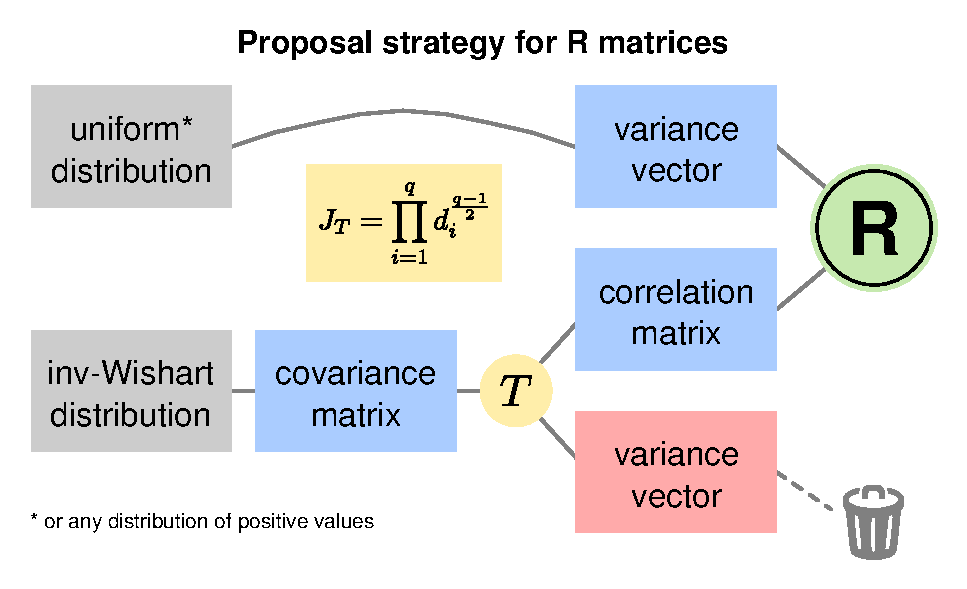
\includegraphics[scale=0.9]{separation_strategy_figure_updated}
	\caption[Diagram of the separation strategy proposal.]{Diagram of the separation strategy proposal \citep{barnard_modeling_2000}. Boxes in grey show the proposal distributions for the variance vector and correlation matrix that compose the evolutionary rate matrix ($\mathbf{R}$). Boxes in blue show the elements that are directly (or indirectly, in the case of the covariance matrix) evaluated in the acceptance step of the MCMC. The yellow circle shows the transformation ($T$) required to decompose the variance-covariance matrix sampled from a inverse-Wishart into a correlation matrix and the variance vector. The yellow square shows the formula for the Jacobian correction due to $T$ \citep{zhang_sampling_2006}, where $d_{i}$ stands for the variance of traits 1 to $q$. The red square demonstrates that a additional variance vector is produced in the process, but it is discarded. The green circle is a representation of the $\mathbf{R}$ matrix as a product between the variance vector and the correlation matrix.}
	\label{fig:proposal}
\end{figure}

\begin{figure}[h]
	\centering
	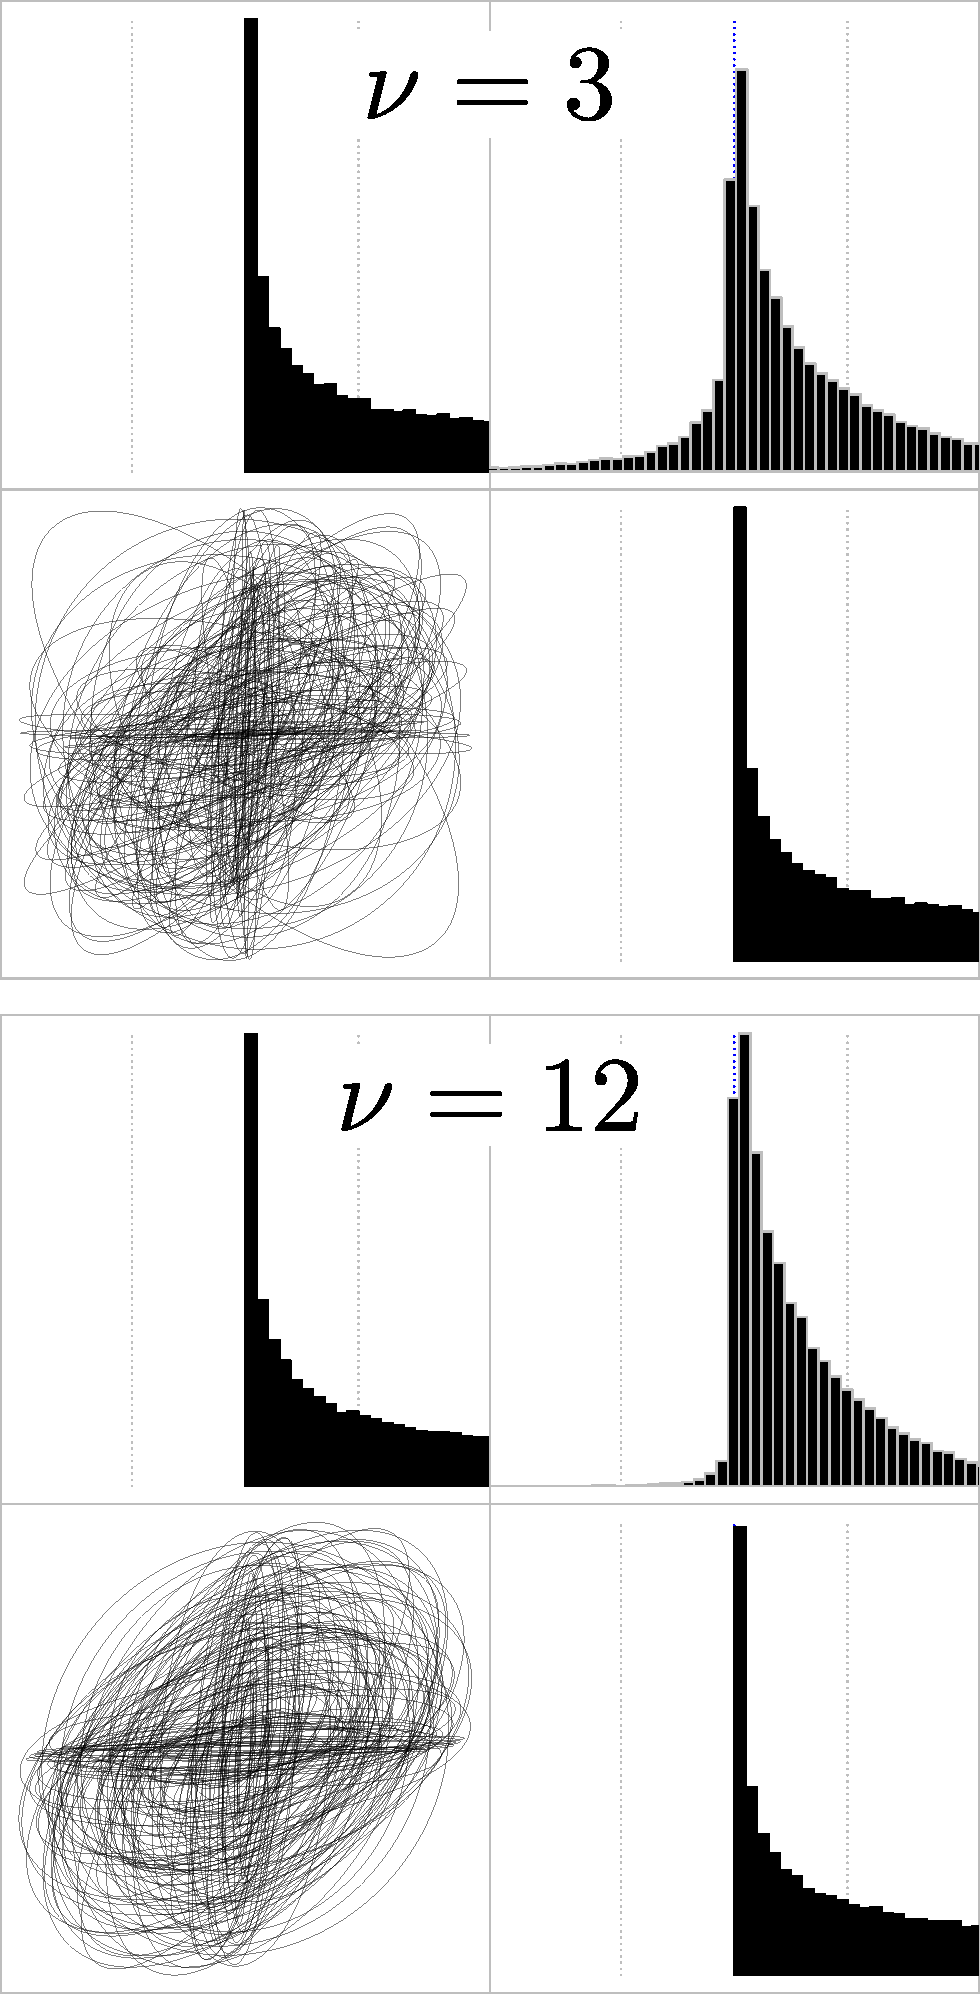
\includegraphics[scale=0.45]{weak_and_strong_prior_mod}
	\caption[Samples from the prior of the evolutionary rate matrix ($\mathbf{R}$) for two simulated traits using the separation strategy.]{Samples from the prior of the evolutionary rate matrix ($\mathbf{R}$) for two simulated traits using the separation strategy \citep{barnard_modeling_2000}. Standard deviation was modelled as a uniform distribution between 0 and 10 and the correlation matrix was derived from a inverse-Wishart centered on a scale matrix with positive correlation (corr = 0.5). Top figure shows a weak prior with small value for the degrees of freedom parameter ($\nu$ = 3) whereas bottom figure are draws from a more informative prior ($\nu$ = 12). In each figure, the plots in the diagonal show evolutionary rates for each trait whereas the upper-diagonal plot shows the evolutionary covariation. Lower-diagonal plot show 150 randomly sampled ellipses representing the 95\% quantile for the bivariate distribution. Although both priors share the same scale matrix, when $\nu$ is small the prior distribution has more variance than when $\nu$ is larger. The diagonal plots are held constant since the prior distribution for the standard deviation is the same in both figures. Note that ellipses show both positive and negative correlation when the prior is weak (top figure) and positive or no correlation when the prior is more informative (bottom figure).}
	\label{fig:prior_samples}
\end{figure}

\begin{figure}[h]
	\centering
	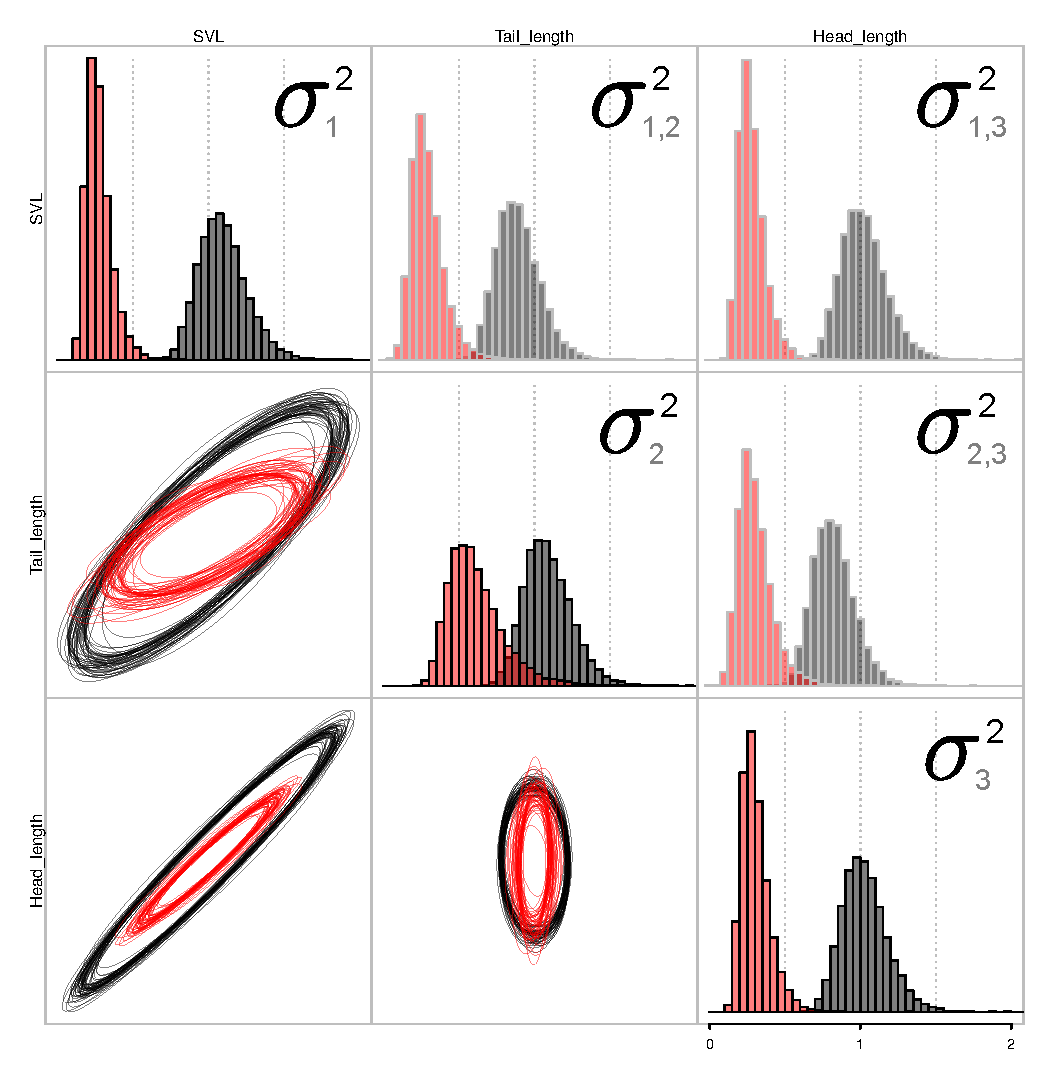
\includegraphics[scale=0.95]{ratematrix_plot_red_and_black_edited}
	\caption[Posterior distribution of the evolutionary rate matrix ($\mathbf{R}$) regimes fitted to the island anole and mainland anole lineages.]{Posterior distribution of the evolutionary rate matrix ($\mathbf{R}$) regimes fitted to the island anole (gray) and mainland anole (pink) lineages. A different $\mathbf{R}$ matrix were jointly estimated for each regime. The plots in the diagonal show evolutionary rates (variances) for each trait; $\sigma_{1}^{2}$ for SVL, $\sigma_{2}^{2}$ for tail length, and $\sigma_{3}^{2}$ for head length. Upper-diagonal plots show pairwise evolutionary covariation (covariances); $\sigma_{1,2}^{2}$ between SVL and tail length, $\sigma_{1,3}^{2}$ between SVL and head length, and $\sigma_{2,3}^{2}$ between tail length and head length. The ellipses in the lower-diagonal plots represent the 95\% confidence interval of each bivariate distribution for 50 randomly sampled $\mathbf{R}$ matrices from the posterior. The order of the ellipse plots is a mirror reflection from the upper-diagonal evolutionary covariance plots. Ellipses are only a sample of the posterior because a very large number of lines can become hard to visualize, however the user can set any number of samples (or the entire posterior).}
	\label{fig:anolesGrid}
\end{figure}

\begin{figure}[h]
	\centering
	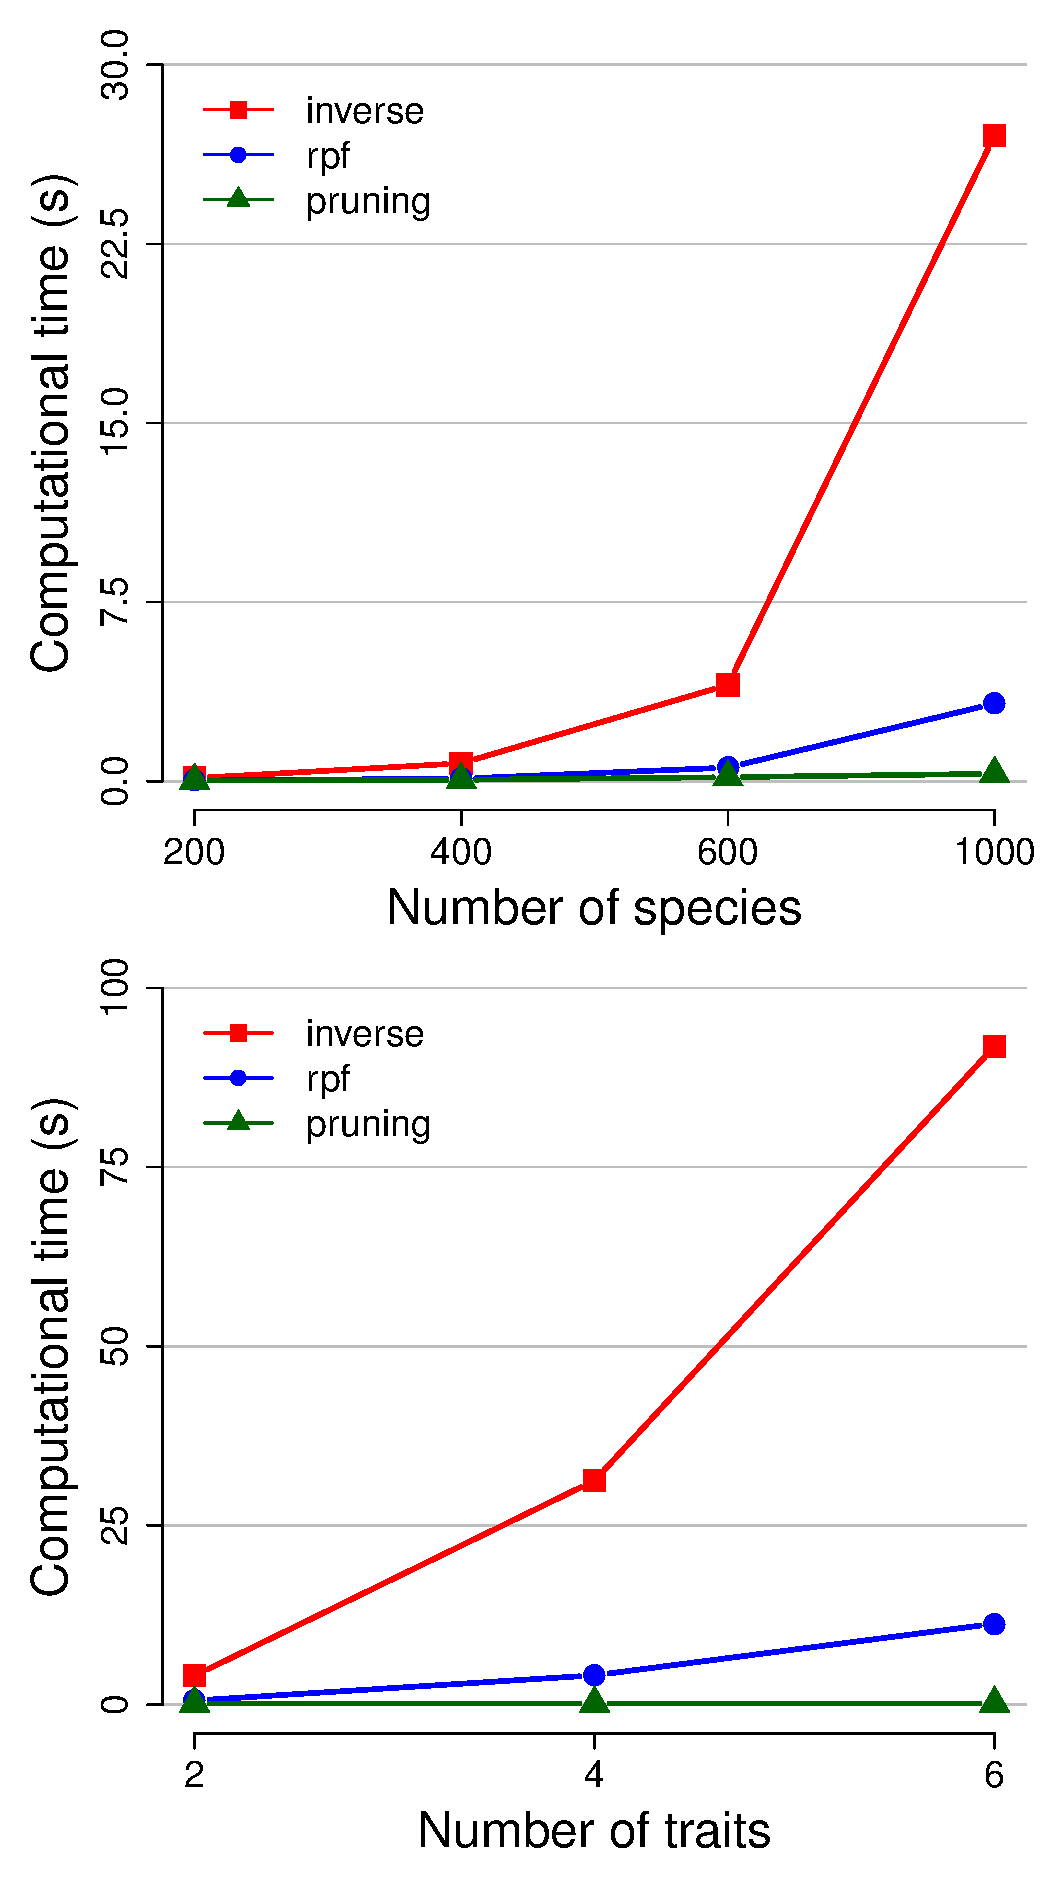
\includegraphics[scale=0.55]{time_plots}
	\caption[Time in seconds spent to compute the likelihood function using different approaches.]{Time in seconds spent to compute the likelihood function using different approaches. Top figure shows computational time for two traits and a phylogeny of different number of species. Bottom figure shows computational time with a phylogeny of 400 species and increasing number of traits. Both plots show a comparison among three approaches: `inverse' uses the full inverse and determinant of matrices as implemented in \texttt{phytools} \citep{revell_phytools:_2012}, `rpf' uses the rectangular full-packed format algorithm as implemented in \texttt{mvMORPH} \citep{Clavel_mvmorph}, and `pruning' uses \citet{felsenstein_1973} pruning algorithm as implemented in \texttt{ratematrix}.}
	\label{fig:time_plot}
\end{figure}

\begin{figure}[h]
	\centering
	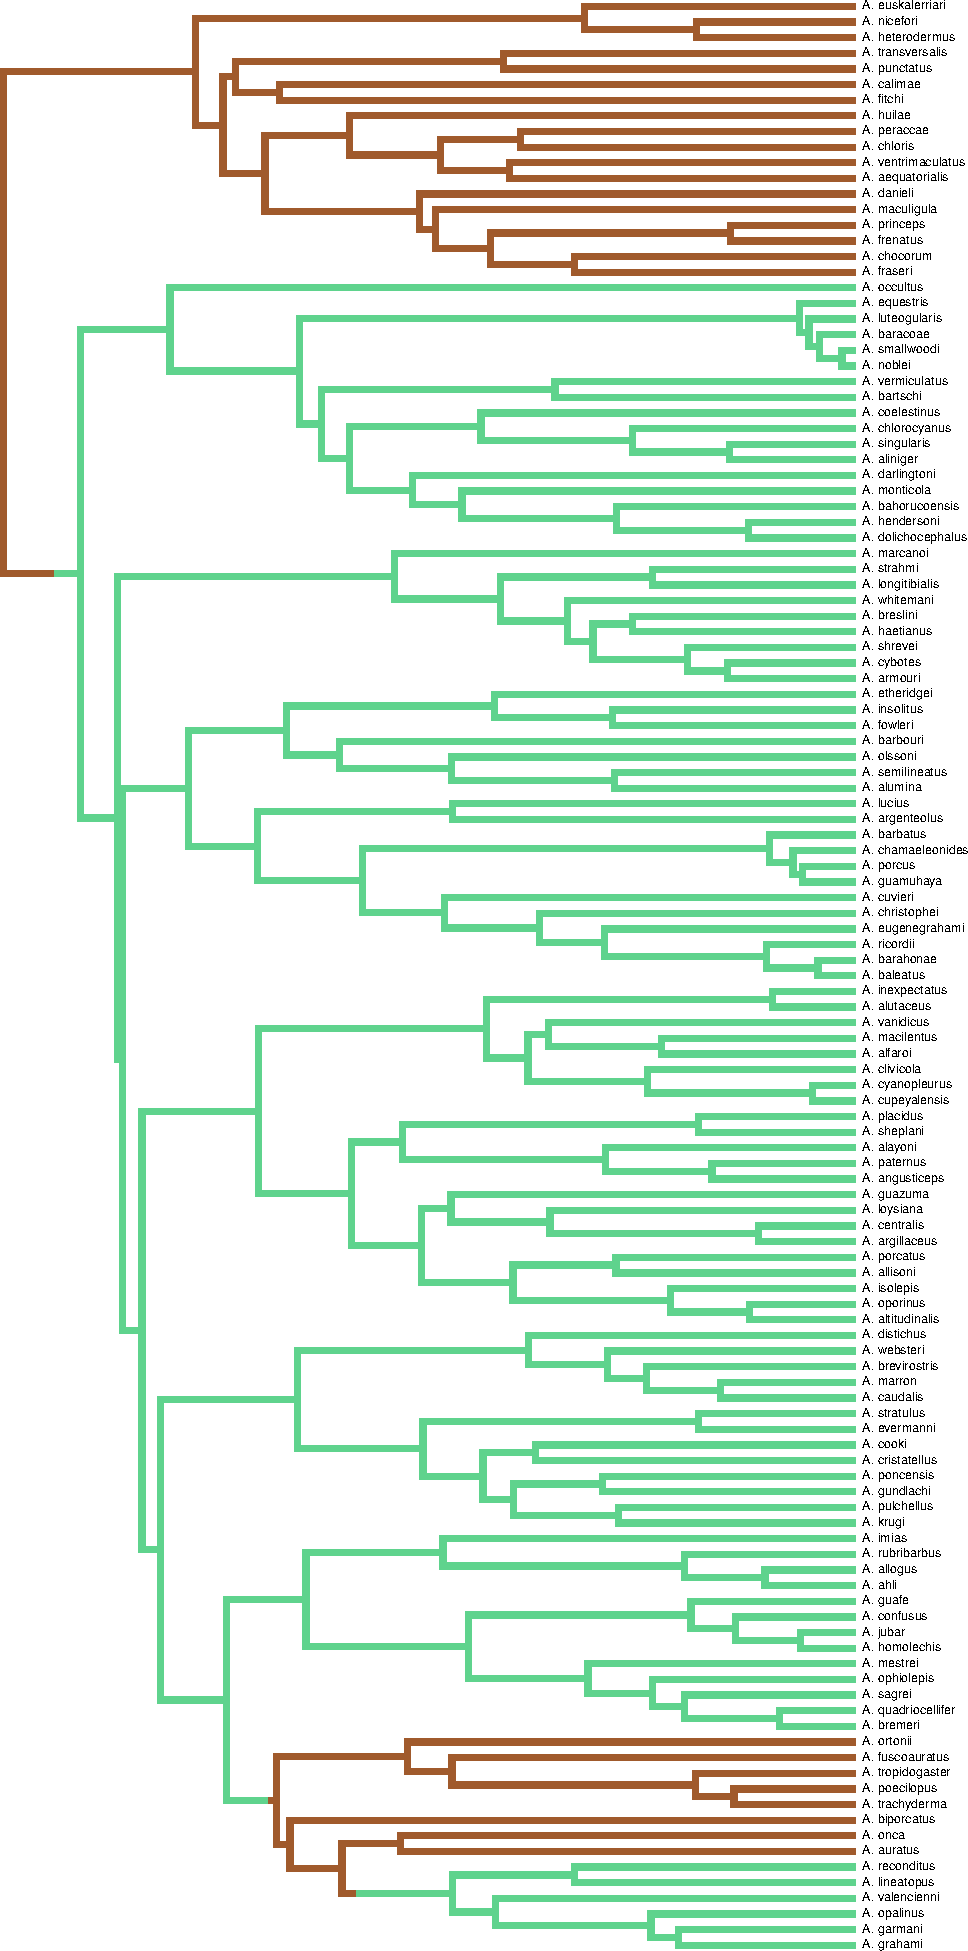
\includegraphics[scale=0.72]{anoles_simmap_tree}
%	\caption[Maximum clade credibility phylogenetic tree for anole lizards made available by \citet{gamble_anolis_2014}.]{Maximum clade credibility phylogenetic tree for anole lizards made available by \citet{gamble_anolis_2014}. Only anole species included in the analysis are shown. Branches painted in brown represent mainland lineages whereas branches in green are island lineages. Regimes were mapped to the tree using stochastic mapping with root state set to mainland, as implemented in the package \texttt{phytools} \citep{revell_phytools:_2012}. Please refer to \citet{caetano_sysbio_2017} for more information.}
%	\label{fig:anoles_simmap}
\end{figure}
\clearpage % insert a page break
\captionof{figure}[Maximum clade credibility phylogenetic tree for anole lizards made available by \citet{gamble_anolis_2014}.]{Maximum clade credibility phylogenetic tree for anole lizards made available by \citet{gamble_anolis_2014}. Only anole species included in the analysis are shown. Branches painted in brown represent mainland lineages whereas branches in green are island lineages. Regimes were mapped to the tree using stochastic mapping with root state set to mainland, as implemented in the package \texttt{phytools} \citep{revell_phytools:_2012}. Please refer to \citet{caetano_sysbio_2017} for more information.}
\label{fig:anoles_simmap}

%% The references for ALL chapters will be at the end of the chapters. The references need to come BEFORE any appendices.
\bibliographystyle{sysbio}
\addcontentsline{toc}{chapter}{Bibliography}
\bibliography{GeoMorpho}

%% Appendices would come here:
% \include{Appendices}

\end{document}